 \documentclass[12pt,fleqn]{amsart}

\usepackage[T1]{fontenc}
\usepackage[utf8]{inputenc}
\usepackage{graphicx}
\usepackage{subcaption}
\usepackage{float}
\usepackage{xcolor}
\usepackage[colorlinks = true, linkcolor = blue]{hyperref}
\usepackage{url}

%Reset the mathcal
\DeclareMathAlphabet{\mathcal}{OMS}{cmsy}{m}{n}
\usepackage{amsmath,amssymb,amsthm,textcomp}
\usepackage{multicol}
\usepackage{multirow}
\usepackage{booktabs}
\usepackage{tikz}
\usepackage[normalem]{ulem}
\usepackage{bbm} % using for the characteristic function

\usepackage{geometry}
\geometry{left=15mm,right=15mm,%
bindingoffset=0mm, top=20mm,bottom=20mm}
\linespread{1.3}
\raggedbottom
\newcommand{\linia}{\rule{\linewidth}{0.5pt}}

\usepackage[open,openlevel=1]{bookmark}

%\newtheorem{theorem}{Theorem}
\newtheorem{theorem}{Theorem}[section]
\renewcommand{\thetheorem}{\arabic{section}.\arabic{theorem}}
\newtheorem{corollary}{Corollary}[theorem]
\newtheorem{lemma}[theorem]{Lemma}
\newtheorem{proposition}[theorem]{Proposition}
\theoremstyle{definition}
\newtheorem{definition}{Definition}[section]
\newtheorem{assumption}{Assumption}[section]
\renewcommand{\thedefinition}{\arabic{section}.\arabic{definition}}
\newtheorem*{example}{Example}
\newtheorem{remark}{Remark}
\allowdisplaybreaks

%algorithm
\usepackage{algorithm}
\usepackage{algorithmic}


%% SYMBOLS
%divergence
\AtBeginDocument{
  \let\div\relax
  \DeclareMathOperator{\div}{div}
}
%contradiction
\usepackage{stmaryrd}
\usepackage{marvosym}
%range
\AtBeginDocument{
  \let\ran\relax
  \DeclareMathOperator{\ran}{ran}
}
%ess span dist
\DeclareMathOperator*{\esssup}{ess\, sup}
\DeclareMathOperator*{\spa}{span}
\DeclareMathOperator*{\dist}{dist}
\DeclareMathOperator*{\atom}{atom}
\DeclareMathOperator*{\cont}{cont}
\DeclareMathOperator*{\sign}{sign}
\DeclareMathOperator*{\supp}{supp}
\DeclareMathOperator*{\dom}{dom}
\DeclareMathOperator*{\cl}{cl}
\DeclareMathOperator*{\relu}{ReLU}
\newcommand{\reluk}{\relu^{k}}

\title[Review]{Review}
\begin{document}
\section{introduction}
The problem under consideration is the dynamic optimal control problem in the space-time domain
\begin{equation}
\label{opt}
\tag{$P$}
\begin{aligned}
	&\inf_{u \in L^2(t_0, T, \mathbb{R}^k)} J(u; t_0, y):= \int_{t_0}^T l(y(t)) + \beta |u(t)|^2 dt, \quad \beta >0\\
	&\text{s.t.}\\
	& \dot{y} = f(y) + g(y) u,\\
	& y(t_0) = x,
\end{aligned}
\end{equation}
where we assume $y(t) \in \mathbb{R}^d, u(t) \in \mathbb{R}^k$, $l \in C^1(\mathbb{R}^d, \mathbb{R}), f \in C^1(\mathbb{R}^d, \mathbb{R}^d), g \in C^1(\mathbb{R}^d, \mathbb{R}^{d \times k})$. 
We assume the minimizer exists.\par

The first method to solve the optimization problem involves computing a state-adjoint-control triple originating from the initial condition $x$, known as the open-loop control. The Pontryagin's Maximum Principle(PMP) yields the first-order optimality condition in the form of a forward-backward coupling Hamilton Jacobi ODE:
\begin{equation}
\label{TPBVP}
\tag{TPBVP}
\left\{
\begin{aligned}
	&\frac{d}{dt}y^* = f(y^*) + g(y^*)u^*,\\
	& y^*(t_0) = x, \\
	& -\frac{d}{dt} p^* = \partial_y \bigg( f(y^*) +  g(y^*) u^* \bigg)^Tp^* + \partial_y l(y^*),\\
	& p^*(T) = 0.
\end{aligned}
\right.
\end{equation}
By the maximality condition of the Hamiltonian at the optimal control we get the optimality condition
\begin{equation}
	u^* = - \frac{1}{2\beta} g(y^*)^T p^* \quad \forall t \in (t_0, T). 
\end{equation}

The optimal trajectories obtained from the solution of the open-loop system are not robust with respect to disturbance \cite{azmi2021optimal}, since the existing numerical methods for two-point boundary value problem in general tend to diverge. 
On the other hand, based on the Dynamic Programming principle,  we introduce the value function 
\begin{align*}
	 V(t, y):= \inf_u J(u; t, y) \quad \text{ subject to the dynamic system},
\end{align*}
which satisfies the nonlinear hyperbolic partial differential equation, the Hamilton-Jacobi-Bellman (HJB) equation:
\begin{equation}
\label{HJB}
\tag{HJB}
\left\{
\begin{aligned}
	& \partial_t V - \frac{1}{4\beta} \nabla V(t, x)^T  g(x) g^T(x) \nabla V (t, x) + \nabla V(t, x)^T f(x) + l(x)  = 0 \\
	& V(T, x) = 0. 
\end{aligned}
\right.
\end{equation}
In this case the optimal control problem becomes solving a nonlinear hyperbolic partial differential equation, which is more robust compared to the open-loop method. 

For most of the nonlinear dynamic control problems, one desires a feedback a feedback control law, which involves solving the optimal value function of 
the HJB equation. 
However, solving the HJB function is notorious difficult since it suffers from the curse-of-dimensionality.
There is an extensive literature on finding the numerical solutions. 
In addition to the classical methods, the data-driven methods have become increasingly poplular. 
One line of works is introduced in \cite{nakamura2021adaptive}, where the training data is generated with (\ref{TPBVP}), and the optimal value function is approximated with the training data.
The optimal feedback laws is later synthesised after validation.
The method effectively overcomes the curse-of-dimensionality, since the data generated is causality-free (not depending on the nearby grid).
Moreover, \cite{azmi2021optimal} (Kunisch et al., 2021) further enrich the data set with the gradient of the value function since a state-adjoint-control triples is generated by solving the open-loop problem provided by the PMP. 
The optimal value function is in turn approximated by hyperbolic cross basis functions with $l^1$ penalty to enhance the sparsity and by the gradient training we get better approximation in the $H^1$ space. 
In terms of different approximation methods besides the hyperbolic basis functions, there is a growing literature on solving the nonlinear optimal control problem using neural networks \cite{lutter2020hjb, shilova2023revisiting}.\par   

In this study the sought for approximating function is given in the form of a two-layer network:
\begin{equation}
	\mathcal{N}_{\omega, c}(x) := \sum_{n = 1}^N c_n \sigma (a_n \cdot x + b_n) \in \mathbb{R},
\end{equation}
where $\sigma$ is a sufficiently smooth activation function and $N$ the width of the network. 
And the gradient is given by: 
\begin{equation*}
	\nabla_x  \mathcal{N}_{\omega, c}(x) =  \sum_{ n = 1}^N c_n \nabla_x \sigma(a_n \cdot x + b_n) \in \mathbb{R}^d .
\end{equation*}

In \cite{azmi2021optimal} the author explored the relationship between (\ref{TPBVP}) and (\ref{HJB}) and suggested a gradient-augmented approach. 
In the data generating process, the adjoint state $p^*$ is obtained as a byproduct of solving (\ref{TPBVP}). 
Moreover, the adjoint state provides the gradient information of the optimal value function: $p^*(t) = \nabla V(t, y^*(t))$ (\cite{cristiani2010initialization} \cite{cannarsa1991some} \cite{clarke1987relationship}). 
Instead of state-value pair we get the dataset of the triple $\{x^i, V(x^i), \nabla V(x^i)\}_{i = 1}^M$ that is enriched with gradient information.
We have the minimization problem
\begin{equation}
\label{lost_dis}
\begin{aligned}
	&\min_{N \in \mathbb{N}, (a_n, b_n, c_n) \in \mathbb{R}^d \times \mathbb{R} \times \mathbb{R}, } l_M (\mathcal{N}_{\omega, c}; V),\\
	& \text{with}\\
	& l_M (\mathcal{N}_{\omega, c}; V) := \frac{1}{2M} \bigg( \sum_{m = 1}^M  |V(x^m) - \mathcal{N}_{\omega, c} (x^m)|^2 +  \sum_{m = 1}^M \sum_{i = 1}^d | \partial_{x_i} V(x^m) - \partial_{x_i} \mathcal{N}_{\omega, c} (x^m) |^2 \bigg),
\end{aligned}
\end{equation}
where $x^m$ is a sample of the random variable $x \in L^2(D, \nu)$ with probability distribution $\nu$ on the domain $D$.
Notice that $N$, the number of neurons, is also an optimization parameter. 
The loss function can be understood as the empirical estimation of the $H^1$ loss
\begin{align*}
	l_\nu (\mathcal{N}_{\omega, c}; V) = \frac{1}{2} \int_D |V(x) - \mathcal{N}_{\omega, c} (x)|^2 + \sum_{i = 1}^d | \partial_{x_i} V(x) - \partial_{x_i} \mathcal{N}_{\omega, c} (x) |^2 d\nu .
\end{align*}

Although the number of neurons don't serve as the inductive bias of the model in general \cite{neyshabur2014search}, sparsity is crucial for the computational efficiency in many problems. 
Furthermore, sparsity is necessary for certain applications, such as deconvolution of point-like objects. 
A sparse learning procedure usually adopts convex reformulation of the problem and employ a sparse promoting convex penalty term on the outer weights, a popular choice is the $l^1$ function (LASSO). 
However it was indicated in  \cite{pieper2022nonconvex}(Pieper et al., 2022) that the convex penalty terms are not able to effectively eliminate the redundancy in a shallow neural network, especially when the neurons are clustering in a small neighborhood. 
A nonconvex sparse learning method is proposed by the author. 
However, in the paper the authors limit the activation function to ReLU. 
The ReLU enjoys many nice properties such as Lipschitz continuity and positive homogeneity, but its second-order weak derivate does not exists as a function while it is a distribution, which makes it infeasible for the gradient training \cite{li2024twolayer}.\par

In this thesis, we develope a data-driven method that harnesses the precision of the gradient training and sparsity promoted by the nonconvex penalty at a higher level.
For the gradient traning, we consider a wider range of the activation functions, including sigmoidal, ReLU-like and tanh form, etc.,  and discuss their approximation propertyies.
In the case of the $k$-homogeneous activation function, we investigate besides the classical nonconvex penalty the fractional exponent penalty. 
After removing the assumptions of bounded dictionary and positive homogeneity of the activation function (or the regularity condition of the penalty), we estabilised the new proofs of existence and optimality conditions, as well as the finite support statement.
We conducted experiments for different problems. By choosing the right activation function and penalty, we achieved better $H^1$ relative error with less neurones. \par

\begin{figure}[H]
\centering
\begin{subfigure}[t]{0.48\textwidth}
\centering
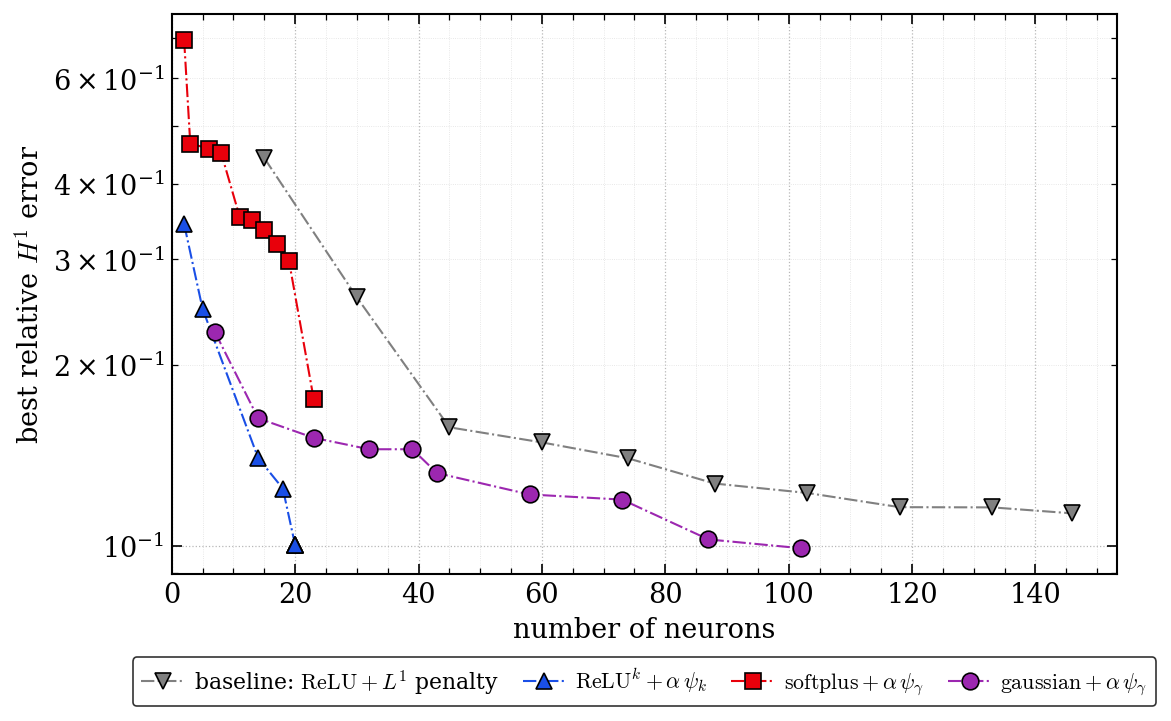
\includegraphics[width=\textwidth]{plot/neuron_h1_frontier_vdp.png}
\caption{Van der Pol oscillator.}
\label{fig:frontier_vdp}
\end{subfigure}
\hfill
\begin{subfigure}[t]{0.48\textwidth}
\centering
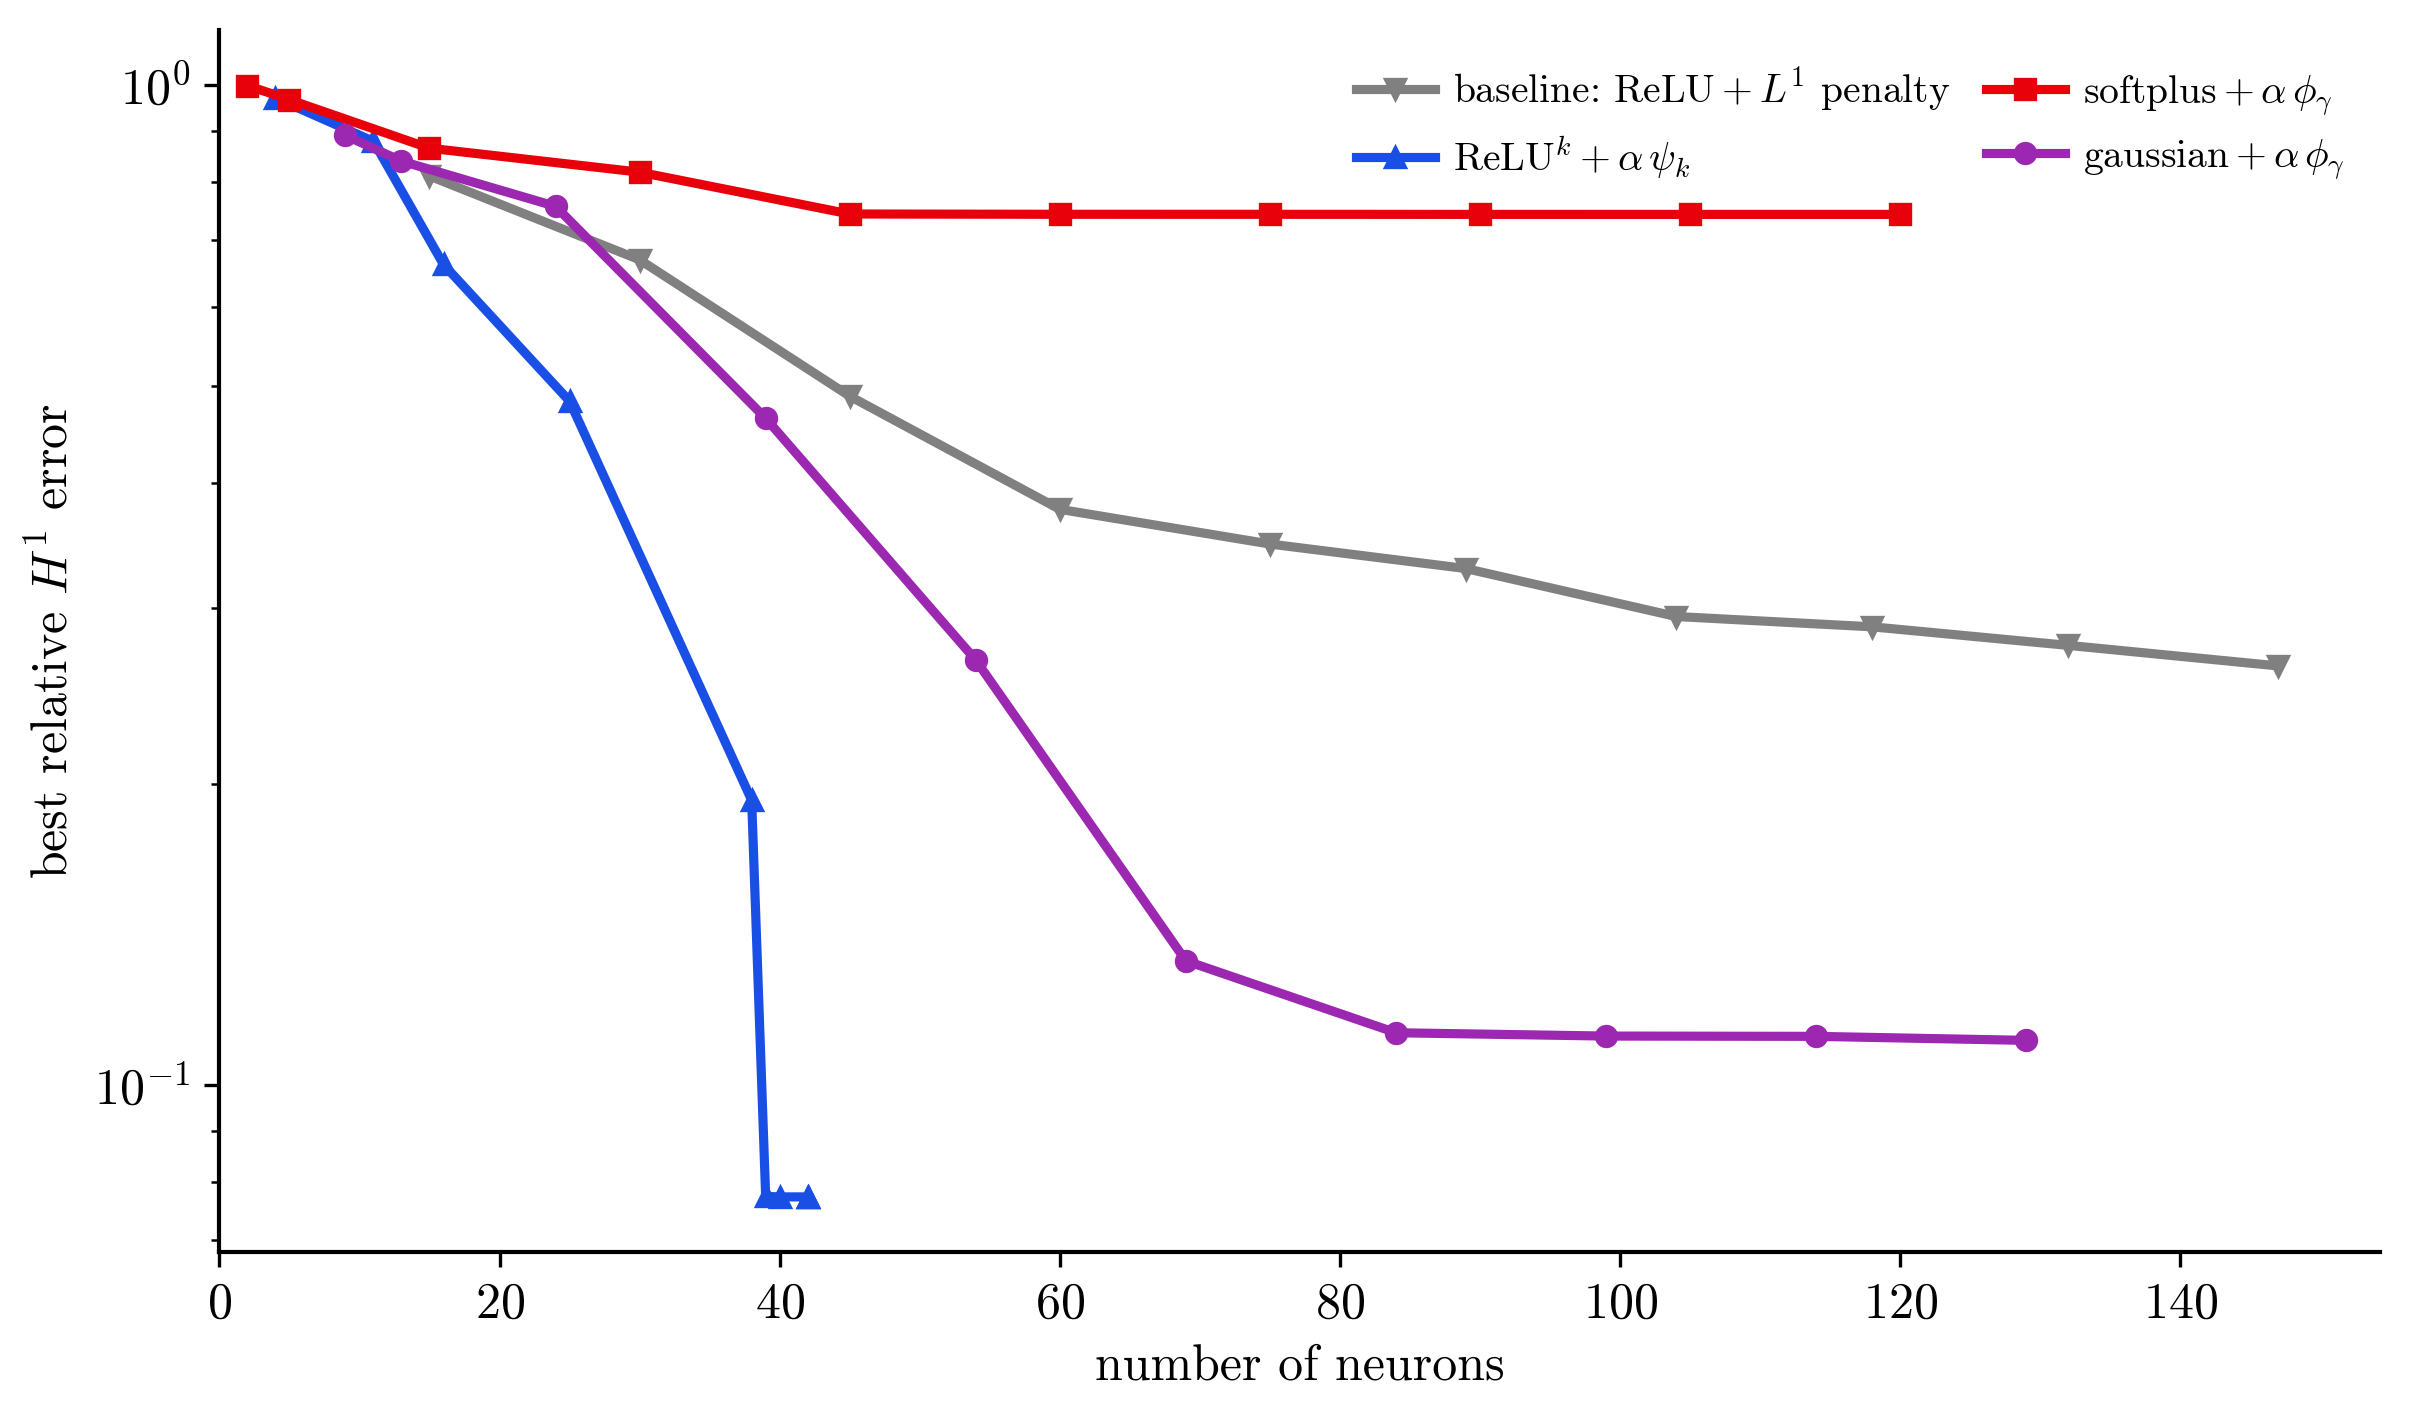
\includegraphics[width=\textwidth]{plot/neuron_h1_frontier_pendulum.png}
\caption{Pendulum swing-up.}
\label{fig:frontier_pendulum}
\end{subfigure}
\caption{Comparison of Number of neurones vs $H^1$ relative error for different optimization problems. The penalty enters as $\alpha \sum$ penalty(|outer weights|). We choose $\alpha = 10^{-5}$, and define the fractional-exponent penalty $\psi(t) = t^{k}$ with $q = \tfrac{2}{k+1} < 1$ (we choose $k = 2$) and the log nonconvex penalty $\phi(t) = \tfrac{1}{\gamma}\log(1 + \gamma t)$(we choose $\gamma = 10$).}
\label{fig:neuron_h1_frontier}
\end{figure}

The general appraoch follows: 
\begin{enumerate}
	\item \textbf{data generation}: initially, a dataset consisting of causality-free state-value-gradient triple must be generated. 
	Many methods are discussed in the literature \cite{kang2021algorithms, barzilai1988two, han2024nonsmooth}.
	The process is highly parallelizable and adaptive. For target regions dense sample set can be selected. 
	\item \textbf{model selection:} depending on the underlying system, different activation function and penalty can be chosen. 
	We have already seen that choices of activation function and regularization impact the model performance significantly. 
	We can also incorporte other prior information such as semiconcavity of the value function or the physics-informed loss \cite{doya2000reinforcement, munos1999gradient, raissi2019physics, tassa2007least, liu2014neural}.
	\item \textbf{training and validataion}: this step will be conducted according to the typical machine learning pipelind. 
	A neural network is trained to approximate the optimal value function, and the performance of the model is subsequently evaluated on a separate validation set. 
	In particular, we can choose the validation set to evaluate the performance on specific areas (such as the switching set of the optimal profile). 
	\item \textbf{feedback control}: once the optimal value function is trained, we can construct the feedback control via PMP. 
	It is in particular effective when the system is high-dimensional. 
	The sparcification facilitates faster computation in the inference stage. 
\end{enumerate}

\section{preliminaries}
Before introducing our optimization problem setting, we give a review about the functional spaces needed for the framework.  
We consider the linear inverse problem of the following type: find $\mu$ such that
\begin{equation*}
	\mathcal{N} \mu = f
\end{equation*}
where $\mu$ is a finite Radon measure and $f$ belongs to some Sobolev space which needs to be specifid. 
Both spaces are important for our analysis. One forms the building blocks of the optimization condition while the other specifies the approximation properties. 

\subsection{Space of Finite Radon Measure}
Throughout the paper we denote $\Omega$ as $\mathbb{R}^{d + 1}$. 
A finite Radon measure $\mu$ is a $\sigma$-additive $\mathbb{R}^m$-valued set function defined on the Borel sets of $\Omega$ with $\mu(\emptyset) = 0$.                                                                              
The \emph{total-variation measure} of a finite Radon measure $\mu$ is the positive measure defined by                                                                                                                                       
\begin{equation*}                                                                                                                                                                                                                                          
|\mu|(E) = \sup \left\{ \sum_{n=1}^{\infty} |\mu(E_n)| \;:\; \bigcup_{n=1}^{\infty} E_n = E,\; \{E_n\} \text{ disjoint and measurable} \right\}.
\end{equation*}
We denote the space of finite Radon measures by $\mathcal{M}(\Omega, \mathbb{R}^m)$ (and $\mathcal{M}(\Omega)$ if $m = 1$). 
The following spaces will be considered
\begin{itemize}
  \item $C_0(\Omega; \mathbb{R}^m)$, the space of all continuous functions $u : \Omega \to \mathbb{R}^m$ \emph{vanishing on the boundary}, that is, for every $\varepsilon > 0$ there exists a compact set $K_\varepsilon \subset \Omega$ such that $|u(x)| < \varepsilon$ for all $x \in \Omega \setminus K_\varepsilon$;
  \item $\mathcal{M}(\Omega; \mathbb{R}^m)$, the space of all vector-valued measures $\mu : \mathcal{B} \to \mathbb{R}^m$ with finite variation on $\Omega$.
\end{itemize}

It is well-known that the space $\mathcal{M}(\Omega, \mathbb{R}^m)$ can be identified as the dual space of $C_0(\Omega; \mathbb{R}^m)$ by the dual pairing:
\begin{equation*}
\langle \mu,\, u \rangle = \sum_{i=1}^{m} \int_\Omega u_i \, \mathrm{d}\mu_i,
\end{equation*}  
The Riesz theorem states that $(C(\Omega, \mathbb{R}^m))^* = \mathcal{M}(\Omega, \mathbb{R}^m)$, which also implies the completeness of the space of finite Radon measures. 
For each $\mu \in \mathcal{M}(\Omega, \mathbb{R}^m)$ and $u \in C(\Omega, \mathbb{R}^m)$.
Without further specification, we denote $\langle \cdot, \cdot\rangle$ the dual bracket $\langle \cdot, \cdot \rangle_{\mathcal{M}(\Omega), C(\Omega)}$. 

The following space of measures will also be considered:
\begin{itemize}
	\item $\mathcal{M}^0(\Omega)$: the space of all nonatomic measures on $(\Omega)$. 
	\item $\mathcal{M}^\sharp(\Omega)$: the space of all purely atomic measures on $\Omega$. 
\end{itemize}

We decompose $\mu \in \mathcal{M}(\Omega)$ by $\mu = \mu_{\cont} + \mu_{\atom}$, where $\mu_{\cont} \in \mathcal{M}^0(\Omega)$ has support $\cont \mu$ and $\mu_{\atom} \in \mathcal{M}^\sharp(\Omega)$ has support $\atom \mu$ \cite{bouchitte1990new}. Therefore we have
\begin{align*}
	\mathcal{M}(\Omega) = \mathcal{M}^0(\Omega) \oplus \mathcal{M}^\sharp(\Omega). 
\end{align*}

\subsection{Barron Space}
In view of the approximation by neural networks, the seminal paper \cite{barron1993universal} develops a universal approximation theorem on function approximation by feedforward neural networks with sigmoidal activation functions.
Later, due to the popularity of ReLU, the universal approximation property of the network with ReLU activation functions is investigated in the subsequent studies \cite{ongie2019function, savarese2019infinite, bengio2005convex, petrosyan2020neural}.
In particular, it is argued that the generalization is achieved by limiting the size of the network, but rather by controlling the magnitute of the weights. 
Let $\mathcal{W}(D)$ be the space of functions $f$ on $D$ that can be representated by $f(x) = \int_{\mathbb{S}^{d}} (a \cdot x + b)_+ d\mu(a, b)$ for every $x \in D$ and some $\mu \in \mathcal{M}(\Omega)$.
For $f \in \mathcal{W}(D)$, we define the norm: 
\begin{equation}
\label{W_norm}
	\|f\|_{\mathcal{W}(D)} = \inf_{\mu \in \mathcal{M}(\Omega)} \|\mu\|_{\mathcal{M}(\Omega)} \quad \text{subject to } f(x) = [\mathcal{N}\mu](x) \text{ for every } x \in D.
\end{equation}

It is shown that the norm is closely related to the fractional Laplacian of $f$ \cite{ongie2019function, savarese2019infinite}.
We want to leverage this norm representation for our gradient training. 
However, we need to reinvestigate the function space since the higher regularity is required for the activation function. 
It is natural to consider $\reluk$ with $k \ge 2$. We introduce the extended Barron norm as in \cite{li2024twolayer}.
For a function $f$ with 
\begin{align*}
	f(x) &= \int_{\mathbb{S}^{d}} (a \cdot x + b)_+^k \, d\mu(a, b),
\end{align*}
and $1\le p < \infty$ we define the representation cost
\begin{equation*}
	\| f \|_{B^k_{p,\mu}} := \left( \int_{\mathbb{S}^{d}} d\mu(a, b)^{kp} \right)^{1/p},
\end{equation*}
and the extended Barron norm
\begin{equation*}
	\| f \|_{B^{k}_{p}} := \inf_{\mu} \| f \|_{B^{k}_{p,\mu}}
	= \inf_{\mu} \left( \sum_{|\alpha| \le k} \left\| \partial^\alpha f \right\|_{B^{k-|\alpha|}_{p,\mu_\alpha}}^{p} \right)^{1/p},
\end{equation*}
where $\alpha$ a multi-index and $\mu_\alpha$ the induced multi-dimensional measures to represent the derivatives.
The infimum is taken over all $\mu$ that represents $f$. 
As before, we define $B_p^k(D)$ to be the space of functions on $D$ with finite Barron norm. 
The Barron space is a normed vector space for $p = 1$. 
The following proposition links the Barron space to the standard Sobolev space.
\begin{proposition}[Barron--Sobolev embedding, {\cite{li2024twolayer}}]
	Given any fixed integer $k$, there holds $B_1^k (D) \subset H^k(D)$.
\end{proposition}

The proposition shows the power and limitation of the Barron space in terms of its representability. 
For the smooth nonlinear systems it yield good approximation. 
However, for the systems with switching profile, it shows limitation (see Figure~\ref{fig:neuron_h1_frontier}).
We can improve the precision by choosing activation that mimics the kinks but the a priori error is always there.

Moreover, the approximation property of other other activation functions with enough smoothness is garanteed by the embedding result of the follwing proportion. 

\begin{proposition}[Embeddings into Barron spaces, {\cite{heeringa2024embeddings}}]
	Let $\sigma$ be a Lipschitz activation function.
	If $\sigma \in C^k(\mathbb{R})$ with $\partial^{k + 1} \sigma \in L^1(\mathbb{R})$, it holds
	\begin{equation*}
		B_\sigma \hookrightarrow B_{\relu^{k}}.
	\end{equation*}
\end{proposition}


\section{the sparse learning problem}
We define the operator $\mathcal{N}: \mathcal{M}(\Omega) \rightarrow H^1(D, \nu) $: 
\begin{align*}
	[\mathcal{N}\mu] (x) = \int_\Omega \sigma (\omega , x) d\mu(\omega).
\end{align*}

Since for all $x$, $\sigma(\cdot, x)$ is bounded by a $\mu$-integrable function , and for all $\omega$, $\sigma(\omega, \cdot )$ is continuous, we can differentiate under the integral sign and get
\begin{align*}
	\nabla_x [\mathcal{N}\mu](x) = \int_\Omega \nabla_x \sigma(\omega,  x) d\mu(\omega). 
\end{align*}

To abuse the notation, we define the operator
\begin{align*}
	\nabla \mathcal{N}: \mathcal{M}(\Omega) \rightarrow L^2(D, \nu)^d, \quad [\nabla\mathcal{N} \mu](x) = \nabla_x[\mathcal{N} \mu](x). 
\end{align*}

In the case that the measure is supported on finite number of atoms, it can be written as
\begin{align*}
	[\mathcal{N}\mu](x) = \sum_{ n = 1}^N c_n \sigma(a_n \cdot x + b_n),
\end{align*}
which is the representation of the neural network, and the gradient of the model is:
\begin{align*}
	[\partial_{x_i} \mathcal{N}](x) = \sum_{n = 1}^N c_n \partial_{x_i} \sigma(a_n \cdot x + b_n).
\end{align*}


Next we incorporate the nonconvex penalty in the integral representation.
For the atom parts it is defined in the discrete setting. 
For the continuous part on $\Omega$ the measure is penalized with the weight $\phi'(0)$. 
Under Assumption \ref{pen1} it is the $L^1$ norm of measure. 
Concretely, observe $\Omega = \atom \mu \cup \cont\mu $, we define the penalty term
\begin{equation}
	\Phi_1(\mu) = \|\mu_{\cont}\|_{\mathcal{M}(\Omega)} + \sum_{\omega \in \atom \mu} \phi(|\mu|(\omega)).
\end{equation}

We formulate now the optimization problem as following:
\begin{equation}
	\label{int_noncon}
	\tag{$P_{\Phi_1}$}
	\left\{
	\begin{aligned}
	& \min_{\mu \in \mathcal{M}(\Omega)} J (\mu):= L(\mu) + \alpha \Phi_1(\mu),\\
	& \text{with},\\
	& L(\mu) = \frac{1}{2} \bigg( \|[\mathcal{N}\mu] - V \|^2_{L^2(D, \nu)} + \sum_{i = 1}^d \|  \partial_{x_i}[\mathcal{N}\mu] - \partial_{x_i} V \|_{L^2(D, \nu)}^2 \bigg) .
	\end{aligned}
	\right.
\end{equation}

We can still perform the gradient-based optimization in the integral setting. 
From the review above we know the gradient is in the space of the continuous function. 

\subsection{The Activation Functions}
First we discuss the choice of activation functions. 
The activations function we consider satisfy the following assumption.
\begin{assumption}[on activation function]
\label{assumption on actfun}
\quad
\begin{enumerate}
\item  $\sigma$ is differentiable w.r.t. $x$. 
\item There exists $ \Lambda > 0$, such that for all $x \in D$, $\omega_1, \omega_2 \in \Omega$, it holds 
\begin{align*}
	&|\sigma(x, \omega_1) - \sigma(x, \omega_2) | \le \Lambda (1 + \|x\|) |\omega_1 - \omega_2|,\\
	& |\partial_{x_i} \sigma(x, \omega_1) - \partial_{x_i} \sigma(x, \omega_2) | \le \Lambda (1 + \|x\|) |\omega_1 - \omega_2| \text{ for all $i = 1, \dots, d$. } 
\end{align*}
\end{enumerate}
\end{assumption}
The Lipschitz continuity of each partial derivative is also required since we are including the gradient information of the value function.

\subsubsection*{Fitting the smooth semiconcave value function}
Because the gradient-augmented loss combines the value error with the gradient error, each neuron $\sigma(\cdot,\omega)$ contributes $\sigma$ to the reconstruction of $V$ and $\partial_{x}\sigma$ to that of $\nabla V$. 
The object relevant to the gradient term is therefore the derivative $\partial_{x}\sigma$, and the approximation efficiency is governed by its shape rather than by that of $\sigma$ itself. 
Figure~\ref{fig:activation_shapes} contrasts three activations admissible under Assumption~\ref{assumption on actfun} through their value, first derivative, and second derivative. 
A monotone, single-signed derivative that stays active over the whole axis (softplus) endows every neuron with a coherent gradient channel of broad, bounded curvature, so that few atoms suffice to represent a smooth $\nabla V$; 
a derivative that saturates on both tails (tanh) supplies only a narrow, localized channel; 
and a localized bump ($e^{-x^2}$) concentrates its curvature near the origin and reverses the sign of its derivative, fitting a smooth field accurately only when densely tiled. 
The regularity of $\partial_{x}\sigma$ should therefore match that of the target gradient field: a smooth, broadly curved derivative suits a smooth value function.

\begin{figure}[H]
\centering
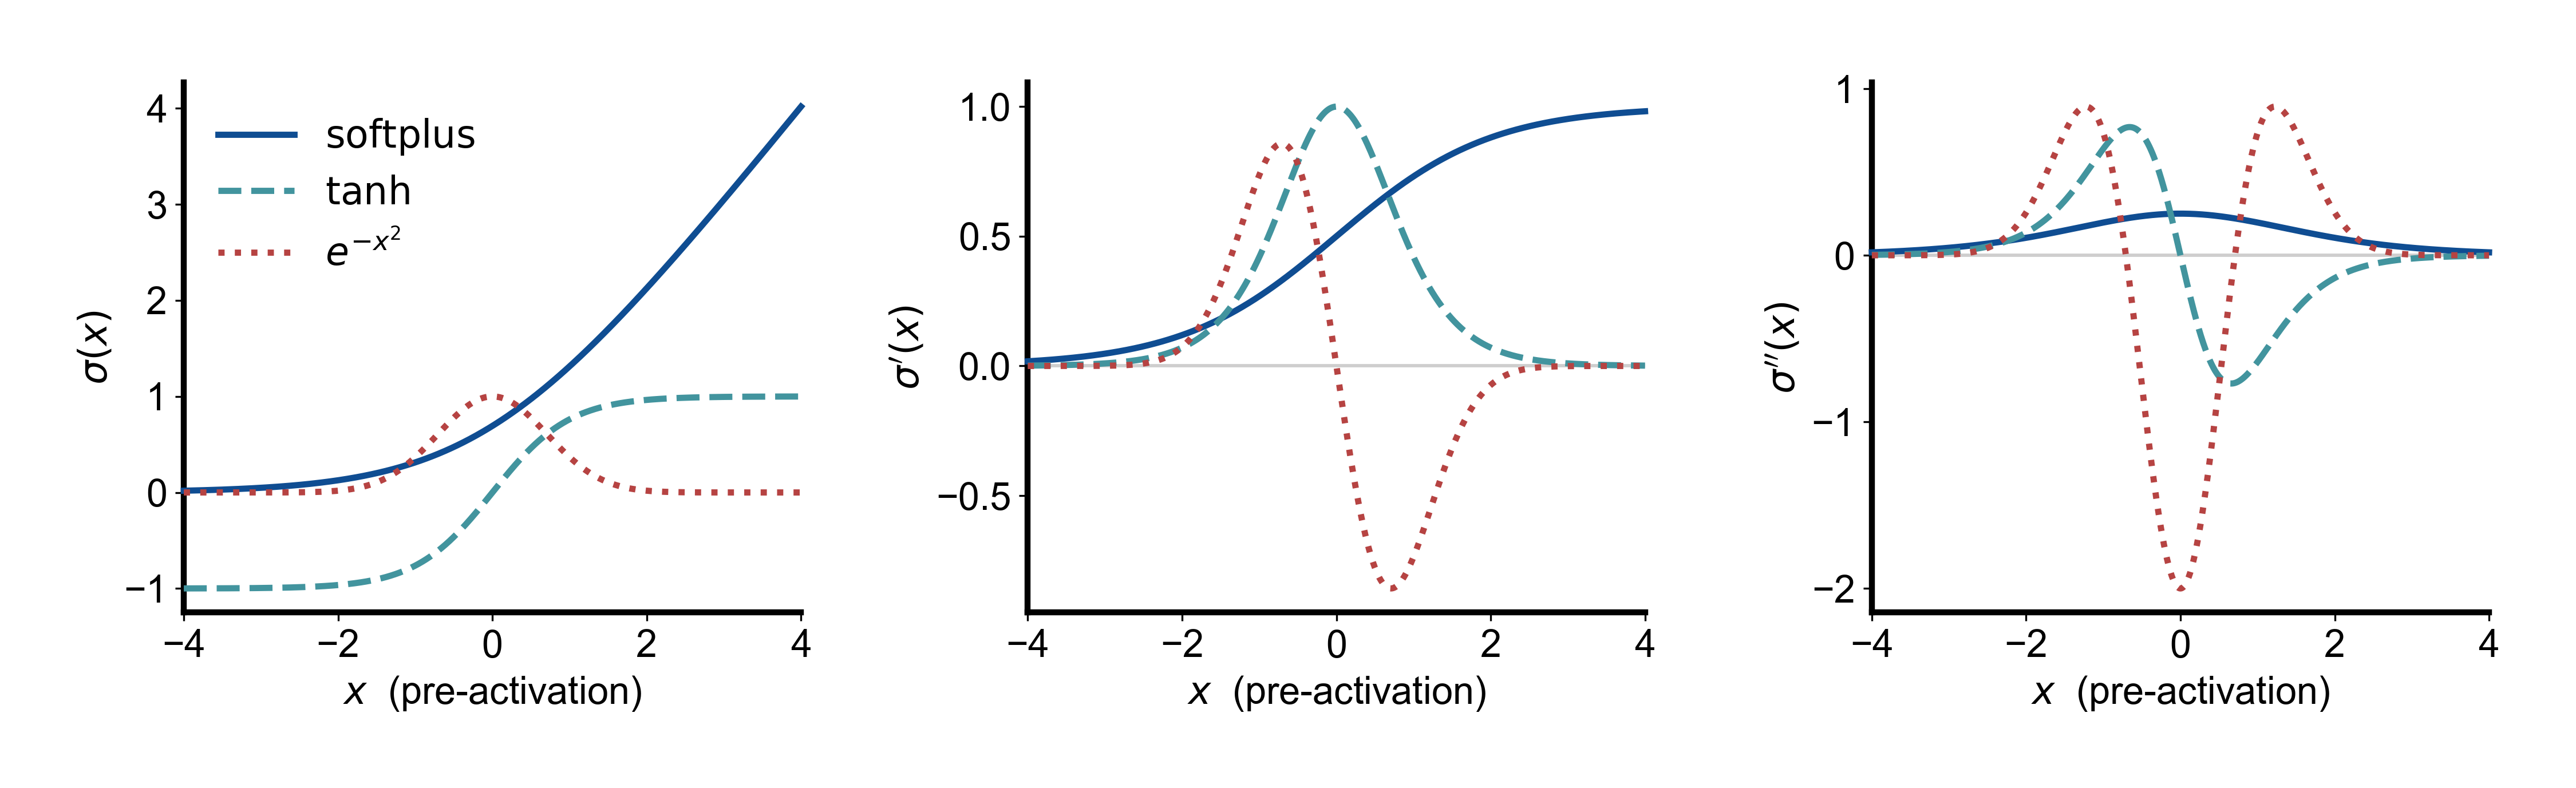
\includegraphics[width=\textwidth]{plot/activation_shapes_smooth.png}
\caption{Three activations admissible under Assumption~\ref{assumption on actfun} --- softplus, tanh, and the Gaussian bump $e^{-x^2}$ --- shown, from left to right, as the value $\sigma$, its first derivative $\sigma'$, and its second derivative (curvature) $\sigma''$ with respect to the pre-activation argument. Under the gradient-augmented loss the first derivative is the basis that reconstructs $\nabla V$.}
\label{fig:activation_shapes}
\end{figure}

\subsubsection*{Fitting the switching set}

When the value function possesses a switching set --- a manifold across which $\nabla V$ is discontinuous, as in the pendulum swing-up problem --- a smooth derivative can no longer reproduce the target gradient field economically. Representing a jump in $\nabla V$ requires a derivative $\partial_{x}\sigma$ that is itself able to break across a hyperplane, which relaxes the differentiability of Assumption~\ref{assumption on actfun}. Figure~\ref{fig:activation_shapes_switching} contrasts three such shapes. The rectified linear unit $\mathrm{ReLU}$ has a step derivative, so a single neuron seats a finite gradient jump exactly on its hyperplane; its squared variant $\mathrm{ReLU}^{2}$ has a kinked but continuous derivative --- a jump in the curvature --- that builds a sharp gradient transition while its quadratic growth still fits the smooth far field, making it the more accurate choice; softplus, whose derivative is smooth, can only smear the jump over a width of order $1/\beta$ and consequently plateaus near the switching set. The positive homogeneity of the rectified families also makes them the natural setting for the sparsity penalty introduced next.

\begin{figure}[H]
\centering
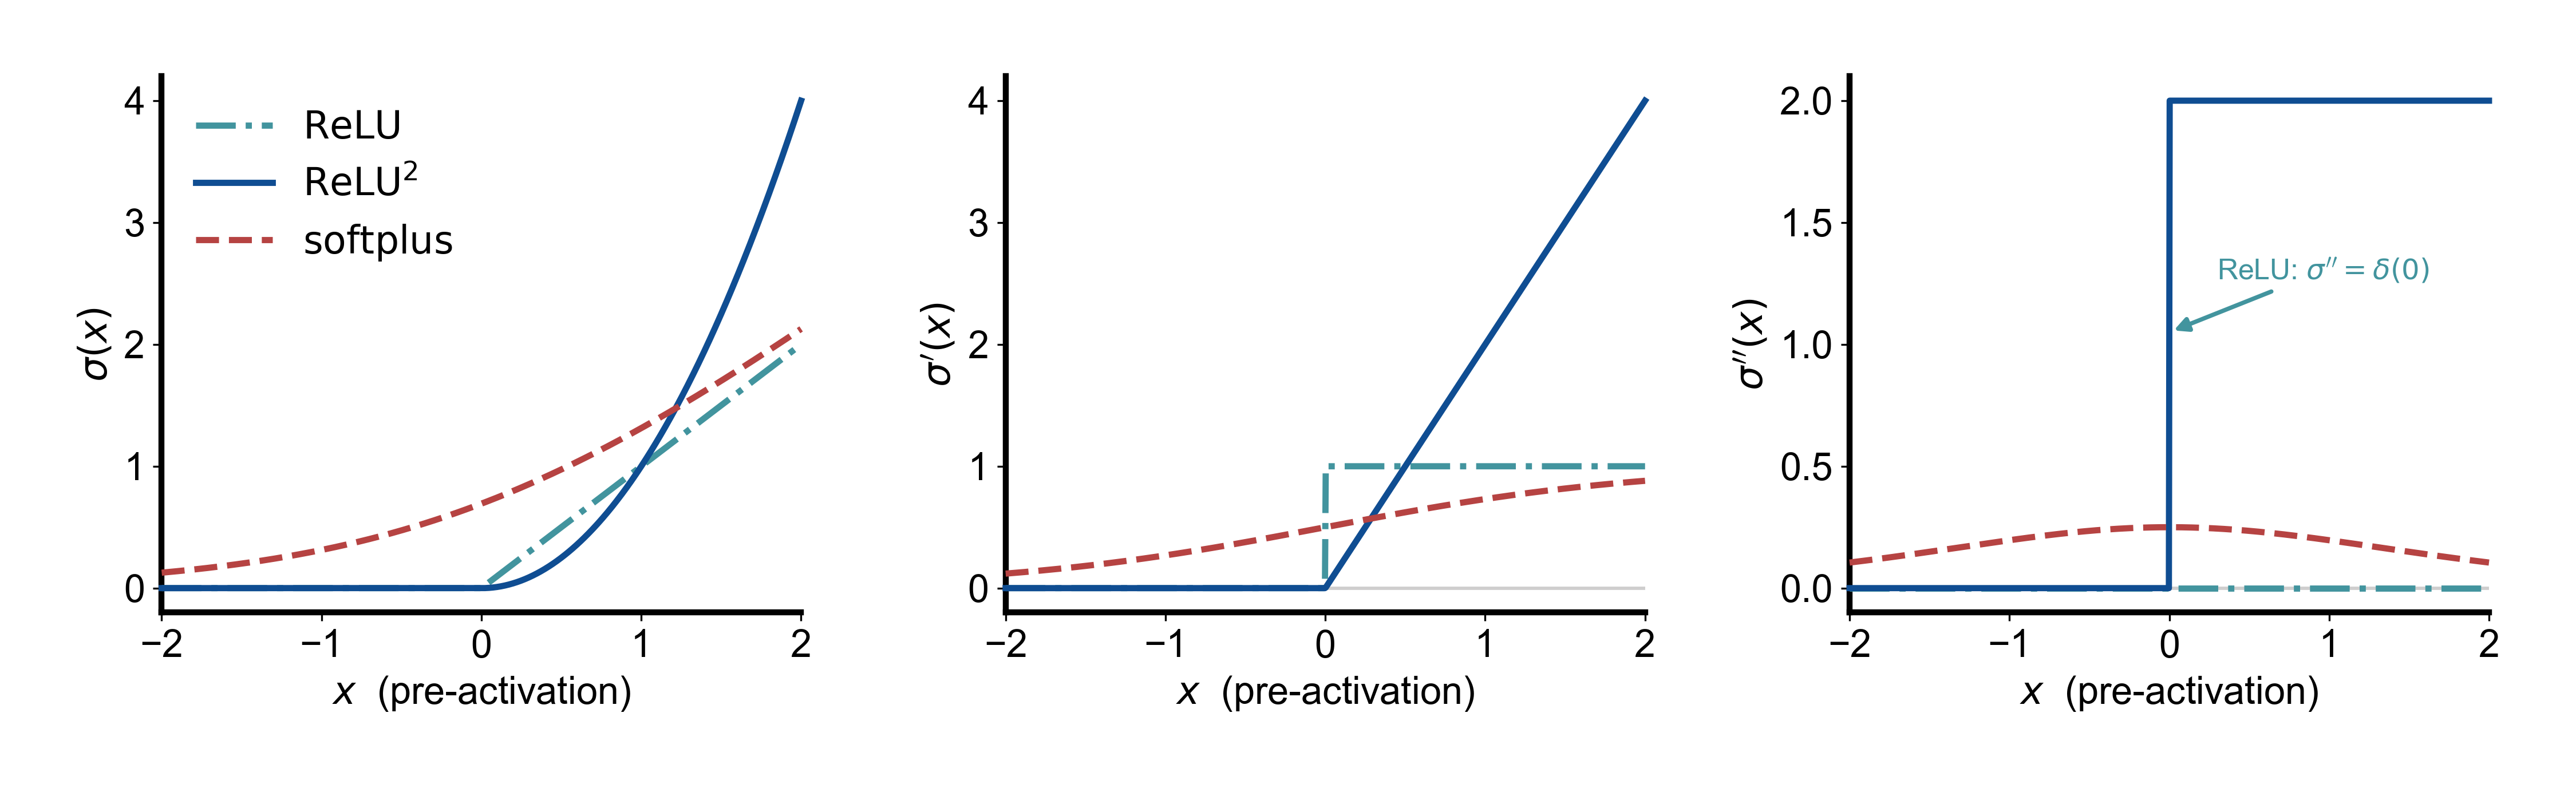
\includegraphics[width=\textwidth]{plot/activation_shapes_discontinuous.png}
\caption{Three activations for a target gradient that jumps across a switching set --- $\mathrm{ReLU}$, $\mathrm{ReLU}^{2}$, and softplus (smooth reference) --- shown, from left to right, as the value $\sigma$, its first derivative $\sigma'$, and its second derivative $\sigma''$ with respect to the pre-activation argument. Only the rectified derivatives can break at the origin: $\mathrm{ReLU}'$ jumps and $(\mathrm{ReLU}^{2})'$ kinks, whereas the softplus derivative is smooth. The curvature of $\mathrm{ReLU}$ is a Dirac mass at the origin (marked).}
\label{fig:activation_shapes_switching}
\end{figure}

\subsection{The Nonconvex Penalty}
We implement an explicit sparsity-promoting penalty term. 
The penalization does not enhance the generalization performance for large neural networks \cite{zhang2021understanding}. 
Nevertheless, the explicit regularization still plays a central role in the sparse learning. 
As introduced in the abstract, the $l^1$ penalty fails to detect the redundancy of the neurons clustering in a small neighborhood, which motivates the nonconvex penalty term. First we introduce the following assumption:
\begin{assumption} \label{pen1}
	The penalty term $\phi: \mathbb{R}_+ \rightarrow \mathbb{R}_+$ satisfies: $\phi$ is differentiable at 0 with $\phi'(0) = 1$. 
\end{assumption}

\begin{assumption} \label{pen2}
The penalty term $\phi: \mathbb{R}_+ \rightarrow \mathbb{R}_+$ is differentiable, concave, nondecreasing and coercive($\phi(z) \rightarrow \infty$ as $z \rightarrow \infty$) with $\phi(0) = 0$.
\end{assumption}
 
The Assumption \ref{pen2} describe the global property of the penalty functions. 
By introducing the nonconvexity the coercivity of the quadratic cost is compromised. 
With Assumption \ref{pen1}, \ref{pen2} the optimization problem stays coercive such that we can apply the direct method of calculus of variation. 
The following lemma follows from the assumption. 
 
\begin{lemma} \label{firstorderestimate} If Assumption \ref{pen2} is satisfied, then it holds
\begin{itemize}
	\item subadditivity: for all $a, b$,  $\phi(a + b) \le \phi(a) + \phi(b)$. 
\end{itemize}
Furthermore, if Assumption \ref{pen1} is satisfied, it holds
\begin{itemize}
	\item $ \phi(z) \le z$.
\end{itemize}
\end{lemma}
\begin{proof}
	\quad\\
	\textbf{1.}  It holds
	\begin{align*}
		\phi(z_1 + z_2) &= \int_0^{z_1} \phi'(z) dz + \int_0^{z_2} \phi'(z_1 + z) dz, \\
(\text{concavity)}\quad		&\le  \int_0^{z_1} \phi'(z) dz + \int_0^{z_2} \phi'(z) dz, \\
\quad		& = \phi(z_1) + \phi(z_2).
	\end{align*}
	\quad\\
	\textbf{2.} it holds for $z \ge 0$:
	\begin{align*}
		\phi(z_1) &= \int_0^{z_1} \phi'(z) dz\\
		 (\phi \text{ concave and } \phi'(0) = 1)  & \le \int_0^{z_1} 1 dz \\
		 &= z_1.
	\end{align*}
\end{proof}
 
 
Assumption \ref{pen1}, \ref{pen2} ensures that the nonconvex problem to admits a global minimizer. 
To enhance the sparsity, we need to exert strong penalizing effect on the weight on 2 neighboring neurons such that merging them would in fact reduce the cost. 
We are mainly interested in the behavior of $\phi'$ in a neighborhood of $0$: 
 
\begin{assumption}[Local concavity]
 \label{pen3}
 The penalty term $\phi: \mathbb{R}_+ \rightarrow \mathbb{R}$ satisfies:
 \begin{enumerate}
  	\item There exists $\gamma_1 \ge 0, \hat{z}_1 > 0$, such that $  -\gamma_1(z_2 - z_1) \le \phi'(z_2) - \phi'(z_1) \le 0$ for all $0\le z_1 \le z_2 \le \hat{z}_1. $ ($\gamma$-convex)
 	\item There exists $\gamma_2 > 0$, $\hat{z}_2 > 0$, such that $\phi'(z_2) - \phi'(z_1) \le -\gamma_2(z_2 - z_1) \le 0 $ for all  $0 \le z_1 \le z_2 \le \hat{z}_2. $ (strongly concave)
 \end{enumerate}
 \end{assumption}
 \begin{remark}
 The Assumption \ref{pen3} can be interpreted as the concave function being strongly concave but exhibits also certain convexity locally at 0. It is worth noticing that it is entirely a local property that only needs to take effect at 0. Assumption \ref{pen3}(2) induces  strict subadditivity that takes effect at small weights. \par
 In general the global concavity in the Assumption \ref{pen2} doesn't imply locally uniform concavity in the Assumption \ref{pen3}(2). 
 Observe, for example $\phi(x) =  x - \frac{2}{3}x^{\frac{3}{2}}$, where the function satisfies the Assumption \ref{pen2} but the locally uniform concavity fails. However since Assumption \ref{pen3} is only local property we may construct piecewise penalty by first constructing the penalty around the neighborhood of 0. 
  
 \end{remark}

\begin{proposition}[the second order estimate]
\label{secondorderestimate}
	Given $\phi$ that satisfies the Assumption \ref{pen1}, \ref{pen2}, if $\phi$ satisfies further Assumption \ref{pen3}, then it holds
	\begin{enumerate}
		\item for all $ z \in [0, \hat{z}_1]: \phi(z) \ge z - \frac{\gamma_1}{2} z^2$, 
		\item for all $z \in [0, \hat{z}_2]: \phi(z) \le z - \frac{\gamma_2}{2}z^2$.
	\end{enumerate} 
\end{proposition}

By the proposition above we know any penalty satisfies Assumption \ref{pen1} and \ref{pen3} admits such upper and lower bound. 
The function
\begin{equation}
	\phi_{\log, \gamma}(z) = \frac{1}{\gamma} \log ( 1 + \gamma z)
\end{equation}
for $\gamma > 0$ and its convex combination with the $l1$ norm will be the main function of choice for our numerical analysis. 



\subsection{Existence of the Global Minimizer}
In this section we prove the existence of the global minimizer. 
We leverage the direct method of calculus variation. 
Since we are working on the space of measure $\mathcal{M}(\Omega)$ we consider the weak-* convergence. 
As usual, the difficulty is to prove the weak-* l.s.c.. 
Furthermore, the coercivity is compromised by introducing the nonconvex penalty term $\Phi$. 
The next lemma address this problem. 
It proves that the coercivity of $\Phi_1$ is preserved by the Assumption \ref{pen1}, \ref{pen2} of $\phi_1$.  

\begin{lemma}[On the coercivity of $\Phi_1$] \label{envolop}
Under the Assumption \ref{pen1}, \ref{pen2}, for any $\mu \in \mathcal{M}(\Omega)$, it holds
\begin{align*}
	\phi_1(\|\mu\|_{\mathcal{M}(\Omega)}) \le \Phi_1(\mu) \le \|\mu\|_{\mathcal{M}(\Omega)}. 
\end{align*}
In particular, the functional $\Phi_1$ is coercive. 
\end{lemma}
\begin{proof}
The proof relies on the subadditivity and $\phi_1(z) \le z$.
\begin{align*}
	\phi_1(\|\mu\|_{\mathcal{M}(\Omega)}) &= \phi_1 \bigg(|\mu|(\Omega \backslash \atom \mu) + \sum_{\omega \in \atom \mu } |\mu|(\{\omega\}) \bigg),\\
	(\text{subadditivity) }
	& \le \phi_1(|\mu|(\Omega\backslash \atom \mu) + \sum_{\omega \in \atom \mu } \phi_1(|\mu|(\{\omega\})), \\
	\bigg(\phi_1(z) \le z\bigg)\quad
	& \le |\mu|(\Omega\backslash \atom \mu) + \sum_{\omega \in  \atom \mu} \phi_1(|\mu|(\{\omega\})),\\
	& = \Phi_1(\mu).
\end{align*}
In particular, by the coercivity of $\phi_1$ it holds that $\Phi_1$ is also coercive. \\
For the second inequality, we leverage that $\phi_1$ is  sublinear and $\phi_1(0)= 0$. We get $\Phi_1(\mu) \le \|\mu\|_{\mathcal{M}(\Omega)}$.  
\end{proof}

The next lemma proves the weak-* l.s.c. of $\Phi_1$.
The proof follows the idea in the paper \cite{bouchitte1990new}.
Since the original proof is valid for $\Omega$ locally compact, the result applies to the current setting.
Moreover, since our functional doesn't have the singular part, the proof and assumptions can be simplified.
\begin{lemma} \label{l.s.c.}
Given $\mu = \mu_{\cont} + \mu_{\atom}$, under Assumption \ref{pen1}, \ref{pen2}, \ref{pen3} it holds
\begin{align*}
	\Phi_1(\mu) = \int_\Omega d\mu_{\cont} + \sum_{ \omega \in \atom \mu } \phi_1(|\mu_{\atom}|(\{\omega\}))
\end{align*}
is weak-* sequentially l.s.c..
\end{lemma}
\begin{proof}
	Let $\mu_h \overset{*}{\rightharpoonup} \mu$, we decompose $\Omega$ by heavy atomes and small atoms combined the continuous part:
	\begin{align*}
		\Omega = A_h + (\Omega - A_h), \text{ where } A_h:= \{ \omega \in \Omega: \mu_h(\omega) \ge \epsilon \}.
	\end{align*}
	By passing to a subsequence we have
	\begin{equation*}
		\mu_{h}|_{A_h} \overset{*}{\rightharpoonup} \mu|_{A_h}, \quad
		\mu_{h}|_{\Omega - A_h} \overset{*}{\rightharpoonup} \mu|_{\Omega - A_h},
	\end{equation*}
	We prove the weak-* l.s.c. of each part. \\
	\textbf{On $ A_h $:} \par
	Since $\mu_h$ has bounded variation and $\mu_h(\omega) \ge \epsilon$ for $\omega \in A_h$, we know the cardinality of $A_h$ is bounded.
	By lemma 3.6 in \cite{bouchitte1990new} we know $M(A_h)$ is sequentially weak-* closed.
	Moreover, $\Phi_1(\mu_h \mathbbm{1}_{A_h})$ is weak-* l.s.c. if $\phi_1$ is l.s.c. and subadditive, therefore we have
	\begin{align*}
		\liminf_{h} \Phi_1(\mu_h \mathbbm{1}_{A_h})
		= \liminf  \sum_{ \omega \in \atom \mu_h \cap A_h } \phi_1(|\mu_{h, \atom}|(\{\omega\}))
		\ge \Phi_1 ( \mu \mathbbm{1}_{A_h}).
	\end{align*}

	\quad\\
	\textbf{On $\Omega - A_h$:} \par
	By proposition \ref{firstorderestimate}, \ref{secondorderestimate}, we have for $\epsilon$ small enough, for all $z \in [0, \epsilon]$:
	\begin{equation*}
		\begin{aligned}
			&\phi_1(z) \ge z - \frac{\gamma_1 z^2}{2}, \\
			&\phi_1(z) \le z.
		\end{aligned}
	\end{equation*}
	We have
	\begin{equation*}
	\begin{aligned}
		&\liminf_h \Phi_1(\mu_h \mathbbm{1}_{\Omega - A_h}) \\
		= & \liminf_h \bigg( \int_{\Omega - A_h} d\mu_{\cont} + \sum_{\omega \in (\Omega - A_h) \cap \atom \mu_h} \phi_1(|\mu_{h, \atom}|(\{\omega\})) \bigg)\\
		\ge & \liminf_h \bigg( \int_{\Omega - A_h} d\mu_{\cont} + \sum_{\omega \in (\Omega - A_h) \cap \atom \mu_h} |\mu_{h, \atom}|(\{\omega\})  - \frac{\gamma_1}{2} |\mu_{h, \atom}|(\{\omega\})^2  \bigg).
	\end{aligned}
	\end{equation*}
	Choose $\delta \ge \frac{\gamma_1}{2} \epsilon$, we have
	\begin{equation*}
		\sum_{\omega \in (\Omega - A_h) \cap \atom \mu_h} |\mu_{h, \atom}|(\{\omega\})  - \frac{\gamma_1}{2} |\mu_{h, \atom}|(\{\omega\})^2
		\ge \sum_{\omega \in (\Omega - A_h) \cap \atom \mu_h} ( 1 - \delta) |\mu_{h, \atom}|(\{\omega\}).
	\end{equation*}
	Hence
	\begin{equation*}
		\begin{aligned}
			&\liminf_h \Phi_1(\mu_h \mathbbm{1}_{\Omega - A_h}) \\
			\ge & \liminf_h (1 - \delta) \int_{\Omega - A_h} d\mu_{\cont} + \liminf_h( 1 - \delta) \sum_{\omega \in (\Omega - A_h) \cap \atom \mu_h} |\mu_{h, \atom}|(\{\omega\})\\
			= & \liminf_h (1 - \delta) \|\mu_h \mathbbm{1}_{\Omega - A_h}\|_{\mathcal{M}(\Omega)}.
		\end{aligned}
	\end{equation*}
	By the weak-* l.s.c. of the norm $\|\cdot\|_{\mathcal{M}(\Omega)}$ we have
	\begin{equation*}
		\liminf_h \Phi_1(\mu_h \mathbbm{1}_{\Omega - A_h}) \ge (1 - \delta) \|\mu \mathbbm{1}_{\Omega - A_h}\|_{\mathcal{M}(\Omega)}.
	\end{equation*}
	Furthermore, applying $\phi_1(z) \le z$ we get
	\begin{align*}
		\sum_{\omega \in (\Omega - A_h) \cap \atom \mu_h}  |\mu_{\atom}|(\{\omega\})
		\ge \sum_{\omega \in (\Omega - A_h) \cap \atom \mu_h} \phi_1(|\mu_{h, \atom}|(\{\omega\})).
	\end{align*}
	Therefore
	\begin{equation*}
		\begin{aligned}
			& \liminf_h \Phi_1(\mu_h \mathbbm{1}_{\Omega - A_h})\\
			\ge & (1 - \delta) \|\mu \mathbbm{1}_{\Omega - A_h}\|_{\mathcal{M}(\Omega)}\\
			\ge & (1 - \delta)\int_{\Omega - A_h} d\mu_{\cont} + \sum_{\omega \in (\Omega - A_h) \cap \atom \mu_h} \phi_1(|\mu_{h, \atom}|(\{\omega\}))\\
			= & (1 - \delta) \Phi_1(\mu \mathbbm{1}_{\Omega - A_h}).
		\end{aligned}
	\end{equation*}
Taking $\epsilon \rightarrow 0$ we get $\delta \rightarrow 0$ and the result is proven. 
\end{proof}

\begin{theorem}[Existence of the global minimizer]
Assuming Assumption \ref{pen1}, \ref{pen2}, \ref{pen3} are fulfilled, problem (\ref{int_noncon}) admits at least one global minimizer in $\mathcal{M}(\Omega)$. 
\end{theorem}
\begin{proof}
We apply the direct method of the calculus of variation:\\ 
1. Boundedness (ability to take a minimizing sequence in $\mathcal{M}(\Omega)$): $J \ge 0$, therefore $J$ is bounded from below.\\
2. Coercivity: By the non-convexity of the penalty term, the coercivity of the cost function is compromised. 
However, we get form lemma \ref{envolop} that $\Phi_1$ is coercive. 
Moreover, $L(\mu)$ is also coercive, hence $J$ is coercive. \\
3. Lower-semi continuity: by the lemma \ref{l.s.c.}  $\Phi_1(\mu)$, is weak-* l.s.c., therefore we have for $\mu_n \overset{*}{\rightharpoonup} \hat{\mu}$,
\begin{align*}
\liminf_{n \rightarrow \infty } J(\mu_n) &= \liminf_{n \rightarrow \infty} \bigg( L(\mu_n)  + \alpha \Phi_1(\mu_n) \bigg)\\
&\ge L(\hat{\mu}) + \alpha \liminf_{n \rightarrow \infty} \Phi_1(\mu_n)\\
& \ge L(\hat{\mu}) + \alpha\Phi_1(\hat{\mu})\\
& = J(\hat{\mu}),
\end{align*}
where the inequality in the second line follows from the weak-* l.s.c. of $L$ (since $L$ is convex and continuous composed with the weak-*-to-weak continuous operator $\mathcal{N}$) and the inequality in the third line follows from weak-* l.s.c. of the functional $\Phi_1$.
\end{proof}
 
\subsection{Optimality Condition and Finite Spport of the Solution}
Since the optimization problem is nonconvex, the global minimizer is difficult to find in general. 
Instead, we define the local minimum: 
\begin{definition}[local minimizer]
$\bar{\mu} \in \mathcal{M}(\Omega)$ is a local minimizer if there exists $\epsilon > 0$ such that 
\begin{align*}
	J(\bar{\mu}) \le J(\mu) \quad \text{for all } \mu \text{ with }  \|\mu - \bar{\mu}\|_{\mathcal{M}(\Omega)} \le \epsilon. 
\end{align*}
\end{definition}

\begin{remark}[The gradient of $L$]
To further investigate the optimality condition of (\ref{int_noncon}) and derive the according algorithm, we calculate the first variation of $L(\mu)$.
We calculate the gradient $\bar{p}(\omega) \in C(\Omega)$:
 \begin{equation}
 \begin{aligned}
 	\bar{p}(\omega) &:= \nabla L(\bar{\mu}) \\
 	& =  \mathcal{N}^*(\mathcal{N}[\bar{\mu}] - V) + \sum_{i = 1}^d (\partial_{x_i} \mathcal{N})^*( \partial_{x_i} \mathcal{N}[\bar{\mu}] - \partial_{x_i} V ) \\
 	& = \int_D \sigma(x, \omega) (\mathcal{N}[\bar{\mu}](x) - V) d\nu(x) + \sum_{i = 1}^d \int_D \partial_{x_i} \sigma(x, \omega) ( \partial_{x_i} \mathcal{N}[\bar{\mu}](x) - \partial_{x_i}V ) d\nu(x) .
 	 \end{aligned}
 \end{equation}
 For the finite sample and $\sigma(x) = \relu(x)^k$, the gradient admits the form:
 \begin{equation*}
 \begin{aligned}
 	p(\omega) ={}& \frac{1}{M} \sum_{m = 1}^M  \relu(\omega \cdot x_m)^k (\mathcal{N}_{\bar{\mu}}(x_m) - y_m) \\
 	&+ \frac{1}{M} \sum_{m = 1}^M \sum_{i = 1}^d k \cdot \relu( \omega \cdot x_m )^{ k -1}  \omega_i (\partial_{x_i} \mathcal{N}(x_m) - \partial_{x_i}V(x_m)).
 \end{aligned}
 \end{equation*}
\end{remark} 
 

\begin{theorem}[the optimality condition]
\label{opt_cdt}
	Under the Assumption \ref{pen1}, \ref{pen2}, if $\bar{\mu}$ is a local minimum of $J$, then it holds
	\begin{enumerate}
		\item $|\bar{p}| \le \alpha \qquad \text{for all } \omega$.
		\item $\bar{p}(\omega) = -\alpha \phi'(|\bar{\mu}|(\omega)) \sign(\bar{\mu}\{ w \}), \qquad \text{for } \bar{\mu}\text{-almost all } \omega \in \Omega.$
	\end{enumerate}
	the signum function $\sign: \Omega \rightarrow \{-1, 1\}$ is defined $\mu$-a.s. by Hahn decomposition. 
\end{theorem}
\begin{proof} 
We leverage that dual evaluation of $\delta_\omega$ is the evaluation of $\bar{p}$ at $\omega$: $\langle \bar{p}, \delta_\omega\rangle_{C(\Omega), \mathcal{M}(\Omega)}= \bar{p}(\omega)$. 
Since $\bar{\mu}$ is the local minimizer, it holds for all $u \in \mathcal{M}(\Omega)$ and $\tau$ small enough:
\begin{align*}
	J(\bar{\mu} + \tau u) - J(\bar{\mu}) = L(\bar{\mu} + \tau u) - L(\bar{\mu}) + \alpha \Phi(\bar{\mu} + \tau u) - \alpha \Phi(\bar{\mu}) \ge 0.
\end{align*}
Taking $\tau \rightarrow 0$, it holds
\begin{align*}
	-\langle \bar{p}, u\rangle \le \alpha \lim_{ \tau \rightarrow 0} \frac{1}{\tau} (\Phi(\bar{\mu} + \tau u) - \Phi(\bar{\mu}) ). 
\end{align*}
Now we separate 2 cases:
\quad\\
\textbf{1)} For the atom part,  $\omega \in \atom \bar{\mu} $ with $\bar{\mu}(\{\omega\}) = c$, taking $u = \delta_\omega$.
it holds
\begin{align*}
	- p(\omega) =  -\langle \bar{p}, u \rangle \le \alpha \lim_{\tau \rightarrow 0} \frac{1}{\tau} (\phi (|c + \tau|) - \phi(|c|) = \alpha \phi'(|c|) \sign(c).  
\end{align*}
Taking $u = \pm \delta_\omega$, we get $p(\omega) = -\alpha \phi'(|c|) \sign(c)$. 
Since $\phi'(0) = 1$ and $\phi'$ is decreasing we have $\phi'(|c|) \in [0, 1]$, hence $|\bar{p}| \le \alpha$. 

\quad\\
\textbf{2)} For the continuous part, first observe $\omega \notin \atom \bar{\mu}$ and perturb with $ u = \delta_\omega$, we have
\begin{align*}
	-\bar{p}(\omega) =  - \langle p, u \rangle \le \alpha \lim_{\tau \rightarrow 0 } \frac{1}{\tau} ( \phi(\tau) - \phi(0) ) = \alpha \phi'(0) = \alpha.
\end{align*}
Taking $u = - \delta_\omega$ we get $|p(\omega)| \le \alpha$ for all $\omega \notin \atom \bar{\mu}$.
Next we take $u = \bar{\mu}_{\text{cont}}$, we have
\begin{align*}
	-\langle \bar{p}, \bar{\mu}_{\text{cont}} \rangle \le \alpha \lim_{\tau \rightarrow 0} \frac{1}{\tau} \tau  \|\bar{\mu}_{\text{cont}}\|_{\mathcal{M}(\Omega)} =  \alpha \|\bar{\mu}_{\text{cont}}\|_{\mathcal{M}(\Omega)}.
\end{align*}
Taking $u = - \bar{\mu}_{\text{cont}}$ we get $-\langle \bar{p}, \bar{\mu}_{\text{cont}} \rangle  = \alpha \|\bar{\mu}_{\text{cont}}\|_{\mathcal{M}(\Omega)}$, i.e., 
\begin{align*}
	\int_\Omega \bigg( - \bar{p}(\omega) * \sign \bar{\mu}_{\cont} (\omega)  - \alpha \bigg) d|\bar{\mu}|(\omega) = 0. 
\end{align*}
By $|p(\omega)| \le \alpha$ we get $\bar{p} =  - \alpha *  \sign \bar{\mu}_{\cont}$ for almost all $\omega \in \cont \bar{\mu}$. 
\end{proof}

The theorem gives a necessary optimality condition for the local minimizer. 
But on the other hand, it lays the ground to prove that the local optimizer admits finite support. 
If the sample size is finite, then the optimal solution admits finite support by the Carath\'eodory's theorem. 
The following theorem proves that the optimal solution admits the finite support even though the dataset is infinitely large. 
Unlike the \cite{pieper2022nonconvex}, we don't assume $\Omega$ is compact. 

\begin{theorem}
	If the Assumption \ref{pen1}, \ref{pen2}, \ref{pen3} are satisfied, then the optimal solution of (\ref{int_noncon}) admits at most finite nodes.
\end{theorem}
\begin{proof}\quad\\
1. $\cont\bar{\mu} = \emptyset$: Argue by contradiction. Assuming there exists $\hat{\omega}$ such that $\bar{\mu}(\{\hat{\omega}\}) = 0$ and $\delta > 0$ such that the open ball $B_\delta(\hat{\omega})$ on $\Omega$ satisfies $|\bar{\mu}|(B_\delta(\hat{\omega})) > 0$. 
Define $D_\delta := B_\delta(\hat{\omega})$ and $C_\delta := |\bar{\mu}|(D_\delta)$ and construct  the measure 
\begin{align*}
	\mu_\delta = \bar{\mu} - \bar{\mu}|_{D_\delta} + C_\delta \delta_{\hat{\omega}}. 
\end{align*}
We prove that the constructed measure decrease the cost function. \par
The cost function is quadratic, therefore the second order Taylor expansion is exact, we get:
\begin{align*}
	L(\mu_\delta)  &= L(\bar{\mu}) + \langle \bar{p}, \mu_\delta - \bar{\mu} \rangle_{C(\Omega), \mathcal{M}(\Omega)} + \frac{1}{2} \|\mathcal{N}[u_\delta - \bar{\mu}]\|_{L^2(D, \nu)}^2 + \frac{1}{2}\sum_{i = 1}^d \|\partial_{x_i} \mathcal{N}[\mu_\delta - \bar{\mu}]\|_{L^2(D, \nu)}^2
\end{align*}
By Assumption \ref{assumption on actfun}, it holds
\begin{align*}
	 |\mathcal{N}[\mu_\delta - \bar{\mu}](x)| &\le \bigg|\int_{D_\delta} \sigma(x, \omega) d\bar{\mu} - C_\delta \sigma(x, \hat{\omega}) \bigg|,\\
	& = \bigg|\int_{D_\delta} \sigma(x, \omega)  - \sigma(x, \hat{\omega}) d \bar{\mu} \bigg|,\\
	& \le \delta \Lambda (1 + \|x\|)|\bar{\mu}|(D_\delta), \\
	& =  \delta \Lambda (1 + \|x\|)C_\delta. 
\end{align*}
Analogously it holds
\begin{align*}
	|\partial_{x_i} \mathcal{N}[\mu_\delta - \bar{\mu}](x)| \le \delta \Lambda (1 + \|x\|)C_\delta.
\end{align*}
Define 
\begin{align*}
	\Lambda_1^2(D, \Lambda) =  \int_D(1 + \|x\|)^2 d\nu  \Lambda^2.
\end{align*}
Hence
\begin{align*}
	L(\mu_\delta) \le L(\bar{\mu}) + \langle \bar{p}, \mu_\delta - \bar{\mu} \rangle + \frac{d + 1}{2}\delta^2 \Lambda_1^2 C_\delta^2. 
\end{align*}
By the Theorem \ref{opt_cdt} $\bar{p}$ is constant for $\omega \in \cont \bar{\mu}$, therefore the first order term vanishes, it holds
\begin{align*}
	L(\mu_\delta) \le L(\bar{\mu})  + \frac{d + 1}{2}\delta^2 \Lambda_1^2 C_\delta^2. 
\end{align*}
Concerning the cost term, it holds
\begin{align*}
	\Phi(\mu_\delta) &= \Phi(\bar{\mu}) - \bar{\mu}(D_\delta) + \phi(C_\delta),\\
	&=\Phi(\bar{\mu}) + \phi(C_\delta) - \bar{\mu}(D_\delta) , \\
	&= \Phi(\bar{\mu}) + \int_0^{C_\delta} \phi'(\xi) - \phi'(0) d\xi,\\
	\text{Assumption \ref{pen3}(2) }
	& \le \Phi(\bar{\mu}) - \frac{ \gamma_2 }{2} C_\delta^2. 
\end{align*}
Combining the 2 parts we get
\begin{align*}
	J(\mu_\delta) \le J(\bar{\mu}) - \bigg(\frac{ \alpha \gamma_2 - (d + 1) \delta^2 \Lambda_1^2}{2} \bigg) C_\delta^2.
\end{align*}
Choose $\delta^2 \le \frac{2 \alpha \gamma_2}{(d + 1)\Lambda_1^2(D, \Lambda)}$ we get the contradiction.

\quad\\
2. $|\atom \bar{\mu}|$ is finite: 
Without loss of generality we can assume the atomic support of $\mu$ is contained in a compact subset of $\Omega$. 
Assume by contradiction, there exists a sequence $\omega_n \rightarrow \infty $ escapes to the infinity.
Since $\bar{\mu} \in \mathcal{M}(\Omega)$ admits bounded variation, by passing to a subsequence, it holds $\bar{\mu}(\omega_n) \rightarrow 0$. 
Assuming w.l.o.g. that $\bar{\mu}(\omega_n) = c_n > 0$, we have
\begin{equation*}
	\begin{aligned}
		\lim_{\omega_n \rightarrow + \infty } \bar{p}(\omega_n)
	= -\alpha \phi'(|\bar{\mu}|(\omega_n)) \sign (\bar{\mu}(\omega_n))
	= - \alpha,
	\end{aligned}
\end{equation*}
which contradicts to that $\bar{p} \in C_0(\Omega)$ and $\lim_{\omega_n \rightarrow + \infty } \bar{p}(\omega_n) \rightarrow 0$.

Now we observe $\atom \bar{\mu}$.
Since it is contained in a compact subset of $\Omega$, there exists a sequence $\omega_n$ (possibly passing through a subsequence) such that 
\begin{align*}
	\omega_n \rightarrow \hat{\omega} \text{ in $\Omega \quad$ for some } \hat{\omega} \in \Omega.
\end{align*}
Assuming w.l.o.g. that $\bar{\mu}(\omega_n) = c_n > 0$, by the boundedness of total variation it holds $ \lim_{n \rightarrow \infty} c_n = 0$. By the Theorem \ref{opt_cdt} , it holds
\begin{align*}
	\bar{p}(\hat{\omega}) = \lim_{n \rightarrow \infty} \bar{p}(\omega_n) = -\alpha \lim_{n\rightarrow \infty} \phi'(c_n) \rightarrow -\alpha.
\end{align*}
Concentrate the measure on $\{\omega_{N}, \dots\}$ on the limits $\hat{\omega}$, i.e., define
\begin{align*}
	\mu_N := \bar{\mu} - \sum_{i = N}^\infty \delta_{\omega_i} \bar{\mu}(\omega_i) + C_N \delta_{\hat{\omega}}, \text{ where } C_N = \sum_{i = N}^\infty c_i > 0.
\end{align*}
As in 1., the fidelity term of the cost can by decomposed by Taylor expansion.\\
Define $\delta_N:= \max_{i = N}^\infty |\omega_i - \hat{\omega}|$ :
\begin{align*}
	L(\mu_N) \le L(\bar{\mu}) + \langle \bar{p}, \mu_N - \bar{\mu}\rangle +\frac{d +1}{2} \Lambda_1^2(D, \Lambda) \delta_N^2  C_N^2
\end{align*}
For the first variation we have by the optimality condition and the argument above:
\begin{align*}
	\langle \bar{p}, \mu_N - \bar{\mu} \rangle = \langle \bar{p},  -\sum_{i = N}^\infty \delta_{\omega_i} \bar{\mu}(\omega_i) + C_N \delta_{\hat{\omega}} \rangle = \alpha \sum_{i = N}^\infty c_i \phi'(c_i) - \alpha C_N.
\end{align*}

For the penalty term, it holds
\begin{align*}
	\Phi(\mu_N) = \Phi(\mu) - \sum_{i = N}^\infty \phi(c_i) + \phi(C_N). 
\end{align*}
Combining the estimation, it holds
\begin{align*}
	J(\mu_N) \le J(\bar{\mu}) - \alpha \sum_{i = N}^\infty \bigg(\phi(c_i) - c_i \phi'(c_i) \bigg) - \alpha\bigg(C_N  - \phi(C_N) \bigg) + \frac{d + 1}{2} \Lambda_1^2(D, \Lambda) \delta_N^2 C_N^2.
\end{align*}
By concavity of $\phi$ it holds
\begin{align*}
	\phi(c_i) - c_i \phi'(c_i) \ge \phi(0) = 0.
\end{align*}
By Assumption \ref{pen3} (2) it holds
\begin{align*}
	C_N - \phi(C_N) &= C_N \phi'(0) - \bigg(\phi(0) + \int_0^{C_N} \phi'(\xi) d\xi \bigg), \\
	(\text{Assumption \ref{pen1}} )
	& = -\int_0^{C_N}\phi'(\xi) - \phi'(0) d\xi, \\
	& \ge \frac{\gamma_2}{2}C_N^2.
\end{align*}
Thus
\begin{align*}
	J(\mu_N) \le J(\bar{\mu}) - \frac{1}{2}\bigg(\alpha \gamma_2 -(d + 1) \Lambda_1^2(D, \Lambda)\delta_N^2 \bigg)C_N^2.
\end{align*}
Taking 
\begin{align*}
	\delta^2 < \frac{\alpha \gamma_2}{\Lambda_1^2(\Lambda, D)(d + 1)},
\end{align*}
we get the contradiction.
\end{proof}

Now we have a necessary optimality condition. But it is not sufficient. More importantly, we cannot formulate an algorithm to determine the optimal value of $N$. To overcome this difficulty, we apply a heuristic approach: For fixed $N$, the optimization problem
\begin{equation}\label{opt_fixN}
	J_{\bar{\omega}}(c):= l(\mathcal{N}_{\bar{\omega}, c}; y) + \sum_{n = 1}^N \phi(|c_n|),
\end{equation}
is well-equipped to solve by traditional gradient-based optimization method. Now we need to find a way to heuristically determine the optimal $\bar{\omega}$ and the optimal number $N$. To this end, we introduce the following theorem as a sufficient condition. 


\begin{theorem}
\label{sc_opt}
 Assuming $\phi$ satisfies the Assumption \ref{pen1}, \ref{pen2}, \ref{pen3}, let $\bar{\mu}$ be a finitely supported measure $\bar{\mu}:= \sum_{n = 1}^N \bar{c}_n \delta_{\bar{\omega}_n}$ such that 
\begin{enumerate}
	\item $\bar{c}_n \in (\mathbb{R} \backslash 0)^N$ is a local minimum of $J_{\bar{\omega}}$, 
	\item For all $\omega \in \Omega \backslash \{\bar{\omega}_n \}_{n = 1, \dots, N}$, it holds $|\bar{p}(\omega)|  \lneqq  \alpha$, where $\bar{p} = \mathcal{N}^*(\mathcal{N}_{\bar{\omega}, \bar{c}} - y) + \sum_{i=1}^d (\partial_{x_i}\mathcal{N})^*(\partial_{x_i}\mathcal{N}_{\bar{\omega}, \bar{c}} - \partial_{x_i} V)$. 
\end{enumerate}
Then $\bar{\mu}$ is a local minimum of $J$.
\end{theorem}
\begin{proof}
For arbitrary $\epsilon > 0$ we observe the open $\epsilon$-ball $B_\epsilon(\bar{\omega}_n)$ around a support point of $\bar{\mu} \in \mathcal{M}(\Omega)$ and define 
\begin{equation*}
    \Omega_\epsilon := \bigcup_{n = 1}^{n = N} B_\epsilon (\bar{\omega}_n)
\end{equation*} 
$\mu \in M (\Omega_\epsilon)$ admits the form:
\begin{align*}
	&\mu = \mu_0 + \tilde{\mu} \quad\text{ with }\quad \mu_0 = \sum_{n = 1}^N c_n \delta_{\bar{\omega}_n},
    \quad 
    \tilde{\mu} = \sum_n \tilde{c}_n \delta_{\tilde{\omega}_n} + \mu_{\cont}\\
	&\text{where}\\
	& \{\tilde{\omega}_n \}_{n = 1}^\infty = \atom \mu \backslash \atom \bar{\mu}, \\
	& c_n = \mu(\{\bar{\omega}_n\}), \tilde{c}_n = \tilde{\mu}(\{\tilde{\omega}_n\}).
\end{align*}

We want to prove for all $\mu \in B_\epsilon(\bar{\mu})$, it holds $J(\bar{\mu}) \le J(\mu)$. First we observe the quadratic fidelity term, it holds
\begin{align*}
	\frac{1}{2}\|\mathcal{N}\mu - y\|_{L^2(D, \nu)}^2 &\ge \frac{1}{2} \|\mathcal{N}_{\bar{\omega}, c} - y\|^2_{L^2(D, \nu)} + \langle \mathcal{N}[\mu_0] - y, \mathcal{N} [\tilde{\mu}] \rangle_{L^2(D, \mu)} + \frac{1}{2}\|\mathcal{N}\tilde{\mu}\|^2_{L^2(D, \nu)} \\
	& \ge \frac{1}{2} \|\mathcal{N}_{\bar{\omega}, c} - y\|^2_{L^2(D, \nu)} + \langle \mathcal{N}[\mu_0 - \bar{\mu}] - y, \mathcal{N}\tilde{\mu} \rangle_{L^2(D, \mu)} + \langle \mathcal{N} \bar{\mu} - y, \mathcal{N} \tilde{\mu}\rangle_{L^2(D, \nu)}\\
	& \ge  \frac{1}{2} \|\mathcal{N}_{\bar{\omega}, c} - y\|^2_{L^2(D, \nu)} - \|\mathcal{N}\|^2 \epsilon \|\tilde{\mu}\|_{\mathcal{M}(\Omega)} + \langle \bar{p}, \tilde{\mu}\rangle.
\end{align*}

For the penalty term, it holds
\begin{align*}
	\Phi(\mu) = \Phi(\mu_0) + \Phi(\tilde{\mu}) = \sum_{n = 1}^N \phi(|c_n|) + \sum_n \phi(|\tilde{c}_n|) + \int_\Omega d|\mu_{\cont}|.
\end{align*}

Choosing $c_n = \bar{c}_n$, the cost thus satisfies
\begin{align*}
	J(\mu) \ge J_{\bar{\omega}}(\bar{c}) - \epsilon \|\mathcal{N}\|^2 \|\tilde{\mu}\|_{\mathcal{M}(\Omega)} + \underbrace{\alpha \Phi(\tilde{\mu}) + \langle \bar{p}, \tilde{\mu} \rangle}_{= (1)}.
\end{align*}

For $(1)$ we estimate
\begin{align*}
	\Phi(\tilde{\mu}) + \langle \bar{p}, \tilde{\mu} \rangle &= \int_\Omega \alpha + \bar{p}(\omega) d|\mu|_{\cont} + \sum_{n} \alpha \phi(|\tilde{c}_n|) + \bar{p}(\tilde{w}_n) \tilde{c}_n \\
	\bigg(|\bar{p}| \le (1 - \delta) \alpha \bigg)
	&\ge  \sum_n \alpha \phi(|\tilde{c}_n|) - (1 - \delta)|\tilde{c}_n| \\
	\bigg(\text{Assumption } \ref{pen3} (1)\bigg)
	&\ge \sum_n \alpha \delta |\tilde{c}_n| -  \frac{\gamma_1 |\tilde{c}_n|^2}{2},
\end{align*}
since $\tilde{c}_n$ is small, the $l^2$ term is dominated by the $l^1$ norm, we have 
\begin{align*}
	\Phi(\tilde{\mu}) + \langle \bar{p}, \tilde{\mu}\rangle \ge (\alpha \delta - \frac{\alpha\gamma_1}{2}) \|\tilde{c}\|_{l^1} \ge (\alpha \delta - \frac{\alpha\gamma_1}{2}) \|\tilde{\mu}\|_{\mathcal{M}(\Omega)} .
\end{align*}
Putting the estimates together, we have
\begin{align*}
	J(\mu) &\ge J(\bar{\mu}) - \bigg(\epsilon \|\mathcal{N}\|^2 + (\alpha \delta - \frac{\alpha\gamma_1}{2}) \bigg) \|\tilde{\mu}\|_{\mathcal{M}(\Omega)}
\end{align*} 
Choose $\epsilon$ such that  $\epsilon \|\mathcal{N}\|^2 + (\alpha \delta - \frac{\alpha\gamma_1}{2}) = 0$ we get the result. 
\end{proof}



\section{the \texorpdfstring{$k$}{k}-homogeneous formulation}
In this section, we discuss a specific class of activation function: the $k$-homogeneous activation function. 

\begin{assumption}[k-homogeneity]
	$\sigma$ is $k$-homogeneous w.r.t. $\omega$ for some $k \ge 2$, i.e., for all $x \in D$, $\lambda > 0$ it holds
\begin{align*}
	\sigma(x, \lambda \omega) = \lambda^k \sigma (x, \omega)\quad \text{ for all } \omega \in \mathbb{R}^{d + 1}.
\end{align*}
\end{assumption}
\begin{remark}
For $k > 2$, the activation function is twice differentiable and the gradient-augmented optimization problem is a smooth optimization problem.
The value part of the loss is approximated by a high-order ReLU activation function $\text{ReLU}^{2 + \epsilon}$, and the gradient by $\text{ReLU}^{1 + \epsilon}$,  for a small $\epsilon$. In the case of $k = 2$, the optimization problem is still well defined but we would have non-differentiable corners for $\partial_{x_i} \sigma$ as in the ReLU case. For $k < 2$, the Lipschitz continuity of the gradient function is compromised.
\end{remark}

\begin{proposition}[Generalization of {\cite[Proposition~3]{pieper2022nonconvex}} to $k$-homogeneous activations]
	Let $p \geq 1$, $q \geq 1$, and let $r \colon \mathbb{R}^{d+1} \to \mathbb{R}_+$ be a positively $1$-homogeneous functional:
	\begin{equation*}
	  r(\tau\,\omega) = |\tau|\, r(\omega) \quad \text{for all } \omega \in \mathbb{R}^{d+1},\; \tau \in \mathbb{R}.
	\end{equation*}
	Suppose the activation function $\sigma(x;\omega)$ is positively $k$-homogeneous in $\omega$, i.e.,
	\begin{equation*}
	  \sigma(x;\, \tau\,\omega) = \tau^k\, \sigma(x;\omega) \quad \text{for all } \tau > 0,\; \omega \in \mathbb{R}^{d+1},\; x \in D.
	\end{equation*}
	Then the unconstrained problem
	\begin{equation*}
	  \min_{N \in \mathbb{N},\; (c_n, \omega_n) \in \mathbb{R} \times \mathbb{R}^{d+1}}
	  \; l(\mathcal{N}_{\omega,c};\, y)
	  + \alpha \sum_{n=1}^{N} \left[ \frac{1}{p}\,|c_n|^p + \frac{1}{q}\,r(\omega_n)^q \right],
	\end{equation*}
	and the sphere-constrained problem
	\begin{equation*}
	  \min_{N \in \mathbb{N},\; \{c_n\} \in \mathbb{R},\; \{\tilde\omega_n:\, r(\tilde\omega_n) \leq 1\}}
	  \; l(\mathcal{N}_{\tilde\omega,c};\, y)
	  + \frac{2\alpha}{s}\, k^{-kp/(kp+q)} \sum_{n=1}^{N} |c_n|^{s/2},
	\end{equation*}
	where
	\begin{equation*}
	  s \;=\; \frac{2pq}{kp + q},
	\end{equation*}
	are equivalent.
\end{proposition}
\begin{remark}\leavevmode
	For $p = q = 2$, the exponent becomes $s/2 = 2/(k+1)$, and the constant is $(k+1)\,k^{-k/(k+1)}$, so the sphere penalty is
	\begin{equation*}
	\alpha\,(k+1)\,k^{-k/(k+1)} \sum_{n=1}^N |c_n|^{2/(k+1)}.
	\end{equation*}
	For $k = 1$ this gives $2\sum|c_n|$; for $k = 2$ this gives $3 \cdot 2^{-2/3}\sum|c_n|^{2/3}$.
\end{remark}
\begin{proof}
	Since $\sigma$ is positively $k$-homogeneous, for any $\tau > 0$ we have
	\begin{equation*}
		c_n\,\sigma(x;\,\omega_n)
		= c_n\,\sigma(x;\,\tau_n\,\tilde\omega_n)
		= c_n\,\tau_n^k\,\sigma(x;\,\tilde\omega_n),
	\end{equation*}
	so $\mathcal{N}_{\omega,c} = \mathcal{N}_{\tilde\omega,\tilde c}$ where $\tilde\omega_n = \omega_n / \tau_n$, $\tilde c_n = c_n\,\tau_n^k$, for any choice of $\tau_n > 0$. In particular, the loss term $l(\mathcal{N}_{\omega,c};\,y)$ is
	invariant under this reparametrization.
	For each $\omega_n \neq 0$, write $\omega_n = \tau_n\,\tilde\omega_n$ with $\tau_n = r(\omega_n) > 0$ and $r(\tilde\omega_n) = 1$ (using the $1$-homogeneity of $r$).
	Then unconstrained problem is equivalent to
	\begin{equation*}
	\min_{\substack{N \in \mathbb{N},\; \{c_n\} \in \mathbb{R}^N \\
	\{\tilde\omega_n:\, r(\tilde\omega_n) \leq 1\},\; \tau_n \geq 0}}
	\; l(\mathcal{N}_{\tilde\omega,\tilde c};\, y)
	+ \alpha \sum_{n=1}^{N}
	\left[ \frac{1}{p}\,\frac{|\tilde c_n|^p}{\tau_n^{kp}} + \frac{1}{q}\,\tau_n^q \right],
\end{equation*}
\quad\\
For fixed $\tilde c_n \neq 0$, define
\begin{equation*}
	g(\tau) \;=\; \frac{1}{p}\,|\tilde c_n|^p\,\tau^{-kp} + \frac{1}{q}\,\tau^q.
\end{equation*}
Since $g(\tau) \to +\infty$ as $\tau \to 0^+$ and $\tau \to +\infty$, the minimum exists and is unique. Differentiating:
\begin{equation*}
	g'(\tau) = -\,k\,|\tilde c_n|^p\,\tau^{-kp-1} + \tau^{q-1} = 0
	\quad\Longleftrightarrow\quad
	\tau^{kp+q} = k\,|\tilde c_n|^p.
\end{equation*}
Hence
\begin{equation*}
	\tau_n^* = \bigl(k\,|\tilde c_n|^p\bigr)^{1/(kp+q)}.
\end{equation*}

\quad\\
Substituting $\tau_n^*$ into $g$:

\emph{First term:}
\begin{equation*}
	\frac{1}{p}\,|\tilde c_n|^p \cdot \bigl(k\,|\tilde c_n|^p\bigr)^{-kp/(kp+q)}
	= \frac{k^{-kp/(kp+q)}}{p}\;|\tilde c_n|^{p\,-\,kp^2/(kp+q)}
	= \frac{k^{-kp/(kp+q)}}{p}\;|\tilde c_n|^{pq/(kp+q)}.
\end{equation*}
Here we used $p - kp^2/(kp+q) = p(kp+q-kp)/(kp+q) = pq/(kp+q)$.

\emph{Second term:}
\begin{equation*}
	\frac{1}{q}\,\bigl(k\,|\tilde c_n|^p\bigr)^{q/(kp+q)}
	= \frac{k^{q/(kp+q)}}{q}\;|\tilde c_n|^{pq/(kp+q)}.
\end{equation*}
Adding the two terms and noting that $pq/(kp+q) = s/2$:
\begin{equation*}
	g(\tau_n^*)
	= \left(\frac{k^{-kp/(kp+q)}}{p} + \frac{k^{q/(kp+q)}}{q}\right) |\tilde c_n|^{s/2}.
\end{equation*}
We simplify the coefficient. Factor out $k^{q/(kp+q)}$:
\begin{equation*}
	\frac{k^{-kp/(kp+q)}}{p} + \frac{k^{q/(kp+q)}}{q}
	= k^{q/(kp+q)}\!\left(\frac{k^{-1}}{p} + \frac{1}{q}\right)
	= k^{q/(kp+q)}\,\frac{q + kp}{kpq}.
\end{equation*}
Since $s = 2pq/(kp+q)$, we have $(kp+q)/(kpq) = 2/(ks)$, so
\begin{equation*}
	g(\tau_n^*) = \frac{2}{s}\,k^{q/(kp+q)}\,k^{-1}\;|\tilde c_n|^{s/2}
	= \frac{2}{s}\,k^{q/(kp+q) - 1}\;|\tilde c_n|^{s/2}
	= \frac{2}{s}\,k^{-kp/(kp+q)}\;|\tilde c_n|^{s/2}.
\end{equation*}
(using $q/(kp+q) - 1 = -kp/(kp+q)$).
\end{proof}

For the $\reluk$ activation function with $k \ge 2$, the penalty term induces the power $2/(k + 1) < 1$. 
The penalty term fails satisfy the Assumption \ref{pen1}, in particular, it holds $\phi_k'(0) = \infty$. 
In this case the penalty functional doesn't have the continuous part. 
The optimization problem becomes:
\begin{equation}
\label{opt_dis_k}
\begin{aligned}
		\min_{N \in \mathbb{N}, \|a_n\|^2 + |b_n|^2 \le  1 , c_n\in \mathbb{R} , n = 1, \dots, N.} l_M(\mathcal{N}_{\omega, c}(x) ;V) + \alpha \sum_{n = 1}^N \phi_k(|c_n|).
\end{aligned}
\end{equation}


The following proposition states that, any optimal solution of (\ref{opt_dis_k}) can be contracted on the unit sphere without increasing its value of the cost function. 
Hence we may constrain the optimization problem to a unit sphere. 
\begin{proposition}[homogeneous reformulation]
Under Assumption \ref{pen2}, assuming (\ref{opt_dis_k}) admits at least 1 global optimal solution and $\sigma$ is $k$-homogeneous with $k \ge 1$, then (\ref{opt_dis_k}) is equivalent to
\begin{equation}
\label{discrete nonconvex problem}
\tag{$P_{\phi_k}$}
		\min_{N \in \mathbb{N}, \|a_n\|^2 + |b_n|^2 =  1 , c_n\in \mathbb{R} , n = 1, \dots, N.} l_M(\mathcal{N}_{\omega, c}(x) ;V) + \alpha \sum_{n = 1}^N \phi_k(|c_n|).
\end{equation}
\end{proposition}
\begin{proof}
    By assumption the optimal solution exists; denote $(\hat{N}, (\hat{a}_n, \hat{b}_n, \hat{c}_n)_{n = 1}^{\hat{N}})$ one of the global minimizers. The optimal value of the first part in the fidelity term is
	\begin{align*}
		 \frac{1}{2M} \sum_{m = 1}^M \bigg|\bigg( \sum_{n = 1}^{\hat{N}} \hat{c}_n \sigma(\hat{a}_n \cdot x_m + \hat{b}_n) \bigg) - V(x_m) \bigg|^2.
	\end{align*}
    For $(\hat{a}_n, \hat{b}_n)$ in the interior of the unit ball with $\|\hat{a}_n\|^2 + |\hat{b}_n|^2 \lneqq  1$ and $(\hat{a}_n,\hat{b}_n)\neq 0$, denote $\lambda_n =\frac{1}{ \sqrt{ \|\hat{a}_n\|^2 + |\hat{b}_n|^2} }\gneqq  1$. Projecting $(\hat{a}_n, \hat{b}_n)$ on the sphere by defining
        \begin{align*}
            (\tilde{a}_n,\tilde{b}_n) = \lambda_n (\hat{a}_n, \hat{b}_n).
        \end{align*}
    Rescaling the outer weights by defining $\tilde{c}_n = \frac{1}{\lambda_n^k} \hat{c}_n$, by $k$-homogeneity of the activation the function value stays the same:
	\begin{align*}
		&\frac{1}{2M} \sum_{m = 1}^M \bigg|\bigg( \sum_{n = 1}^{\hat{N}} \tilde{c}_n \sigma(\tilde{a}_n \cdot x_m + \tilde{b}_n) \bigg) - V(x_m) \bigg|^2 \\
		&\qquad= \frac{1}{2M} \sum_{m = 1}^M \bigg|\bigg(\sum_{n = 1}^{\hat{N}} \hat{c}_n \frac{1}{\lambda_n^k}  \lambda_n^k \sigma(\hat{a}_n \cdot x_m + \hat{b}_n) \bigg) - V(x_m) \bigg|^2 \\
		&\qquad= \frac{1}{2M} \sum_{m = 1}^M \bigg|\bigg( \sum_{n = 1}^{\hat{N}} \hat{c}_n \sigma(\hat{a}_n \cdot x_m + \hat{b}_n) \bigg) - V(x_m) \bigg|^2.
	\end{align*}
    The fidelity is invariant w.r.t. the scaling. A similar result holds for the second part of the fidelity term by linearity
	\begin{align*}
		\tilde{c}_n \nabla_x \sigma (\tilde{a}_n \cdot x + \tilde{b}_n) = \hat{c}_n \frac{1}{\lambda_n^k} \nabla_x \bigg(\lambda_n^k \sigma(\hat{a}_n \cdot x+ \hat{b}_n) \bigg) = \hat{c}_n \nabla_x \sigma(\hat{a}_n \cdot x + \hat{b}_n).
	\end{align*}

    On the other hand, the penalty term is nondecreasing by Assumption \ref{pen2}. Since $\lambda_n > 1$ and $k \ge 1$, it holds $|\tilde{c}_n| = |\hat{c}_n|/\lambda_n^k \le |\hat{c}_n|$, hence
	\begin{align*}
		\phi_k(|\tilde{c}_n|) \le \phi_k(|\hat{c}_n|).
	\end{align*}
	The pair $\bigg(\tilde{N}, (\tilde{a}_n, \tilde{b}_n, \tilde{c}_n)_{n = 1}^{\tilde{N}} \bigg)$ with
	\begin{align*}
		\tilde{N} = \hat{N} \in \mathbb{N},\quad (\tilde{a}_n,\tilde{b}_n) \in \mathbb{S}^d, \quad \tilde{c}_n \in \mathbb{R}, \quad n = 1, \dots, \tilde{N},
	\end{align*}
	is feasible for the sphere-constrained problem and yields a value no larger than the optimum of (\ref{opt_dis_k}).
\end{proof}

\subsubsection*{The $\reluk$ function}
First we consider the ReLU function with the power $k$:
\begin{align*}
	\sigma(x, \omega) = \max\{0, \omega \cdot x\}^{k}, \text{ with } k \in [2, \infty).
\end{align*}
Since they are not polynomial, they can linearly approximate any measurable function \cite{leshno1993multilayer}.
In this case the gradient is
\begin{align*}
	\nabla_x \sigma(x, \omega) =
	\begin{bmatrix}
		k \max\{0, \omega \cdot x \}^{k - 1} \omega_1\\
		k \max\{0, \omega \cdot x \}^{k - 1} \omega_2 \\
		\dots \\
		k \max\{0, \omega \cdot x \}^{k - 1} \omega_d
	\end{bmatrix} \in \mathbb{R}^d.
\end{align*}

The activation function is non-decreasing and positive homogeneous of degree $k$.
For the standard ReLU activation ($k = 1$), the second-order weak derivative of an approximant $f_n$ fails to exist as a function (it is only a distribution), so $f_n$ cannot be used to mimic higher-order derivatives.
Choosing $\sigma$ as a $\mathrm{ReLU}^k$ activation with $k > 1$ remedies this and enables simultaneous approximation of a function together with its derivatives.

For $k > 1$,  the activation function not only preserves the nice property such as homogeneity of ReLU, but also smooths the kinks. We gain 2 things from the differentiability: 1. It circumvents the non-differentiable corners of the ReLU function; 2. The gradient information of the activation function can be used to calculate the gradient-augmented loss function. More generally, we assume the activation function to satisfy the following condition:






In absence of Assumption \ref{pen1}, it is difficult to prove the existence of the global optimizer with the direct method of . 
For example for the penalty $ \phi(c) = |c|^q$ with $q < 1$, we have $\phi'(0) = \infty$, the weak-* l.s.c. of the cost functional breaks.
However, assuming the local optimizer exists, we can still derive the necessary optimality condition. 

\begin{corollary}[Optimality conditions for $\phi'(0^+) = +\infty$]                     
\label{cor:singular_penalty}                                                                                                                                                                                                                
Let $\Omega$ be compact and suppose $\phi$ satisfies Assumption~\ref{pen2} but with $\phi'(0^+) = +\infty$ in place of Assumption~\ref{pen1}                                                                                                
(e.g., $\phi(z) = \frac{1}{q}z^q$ for $0 < q < 1$).                                                                                                                                                                                         
If $\bar{\mu}$ is a local minimizer of \eqref{int_noncon} with atomic part                                                                                                                                                                  
$\bar{\mu}_{\atom} = \sum_{n=1}^N \bar{c}_n\,\delta_{\bar{\omega}_n}$, $\bar{c}_n \neq 0$, then:
\begin{enumerate}
	\item Stationarity at each atom:
	\begin{equation*}
		\bar{p}(\bar{\omega}_n) = -\alpha\,\phi'(|\bar{c}_n|)\,\sign(\bar{c}_n),
		\qquad n = 1, \dots, N.
	\end{equation*}

	\item Lower bound on atom weights:
	Since $\bar{p} \in C(\Omega)$ and $\Omega$ is compact,
	$\|\bar{p}\|_{C(\Omega)} < \infty$.
	Combined with (1), this gives
	$\phi'(|\bar{c}_n|) = |\bar{p}(\bar{\omega}_n)|/\alpha \le \|\bar{p}\|_{C(\Omega)}/\alpha$
	for every $n$. Since $\phi'$ is decreasing with $\phi'(0^+) = +\infty$,
	inverting yields a uniform lower bound:
	\begin{equation*}
		|\bar{c}_n| \;\ge\; (\phi')^{-1}\!\Big(\frac{\|\bar{p}\|_{C(\Omega)}}{\alpha}\Big)
		\;>\; 0,
		\qquad n = 1, \dots, N.
	\end{equation*}
	In particular, $\bar{\mu}$ has at most finitely many atoms:
	$N \le \|\bar{\mu}\|_{\mathcal{M}(\Omega)} \big/ \min_n |\bar{c}_n| < \infty$.
\end{enumerate}
\end{corollary}
\begin{proof}
(1) follows by the same directional derivative argument as in Theorem~\ref{opt_cdt}.
For $\omega_n \in \atom\bar{\mu}$ with $\bar{\mu}(\{\omega_n\}) = \bar{c}_n \neq 0$,
perturbing with $u = \pm\delta_{\omega_n}$ gives
\begin{equation*}
	\mp\,\bar{p}(\omega_n)
	\;\le\; \alpha\,\lim_{\tau \to 0}\frac{1}{\tau}
	\bigl[\phi(|\bar{c}_n \pm \tau|) - \phi(|\bar{c}_n|)\bigr]
	\;=\; \pm\,\alpha\,\phi'(|\bar{c}_n|)\,\sign(\bar{c}_n),
\end{equation*}
which yields equality. Note that $\phi'(|\bar{c}_n|) < \infty$ for $\bar{c}_n \neq 0$,
so this step does not require $\phi'(0) < \infty$.

\medskip\noindent
(2): The dual variable $\bar{p} = \nabla L(\bar{\mu}) \in C(\Omega)$
is continuous on the compact set $\Omega$, hence bounded:
$\|\bar{p}\|_{C(\Omega)} < \infty$.
By (1), $\phi'(|\bar{c}_n|) = |\bar{p}(\bar{\omega}_n)|/\alpha
\le \|\bar{p}\|_{C(\Omega)}/\alpha$.
Since $\phi'$ is strictly decreasing (by concavity of $\phi$) and
$\phi'(0^+) = +\infty$, the function $\phi'$ restricted to $(0,\infty)$
has a well-defined decreasing inverse, and
\begin{equation*}
	|\bar{c}_n| \;\ge\; (\phi')^{-1}\!\Big(\frac{\|\bar{p}\|_{C(\Omega)}}{\alpha}\Big)
	\;=:\; c_{\min} \;>\; 0.
\end{equation*}
The finiteness of the support then follows from the bounded total variation:
$N \cdot c_{\min} \le \sum_{n=1}^N |\bar{c}_n| \le \|\bar{\mu}\|_{\mathcal{M}(\Omega)} < \infty$.
\end{proof}

\begin{remark}
Compared with Theorem~\ref{opt_cdt}:
\begin{enumerate}
	\item The global dual bound $|\bar{p}(\omega)| \le \alpha$ for all $\omega \in \Omega$
	is \emph{lost}: for $\omega \notin \atom\bar{\mu}$, perturbing with
	$u = \delta_\omega$ yields
	$-\bar{p}(\omega) \le \alpha\,\phi'(0^+) = +\infty$, which is vacuous.
	No constraint on $\bar{p}$ is obtained away from the support.
	\item In exchange, the singularity $\phi'(0^+) = +\infty$ provides an
	\emph{automatic minimum atom size} via (2), and finite support
	follows without the merging argument of Theorem~5.2 or
	the local strong concavity in Assumption~\ref{pen3}.
	\item The zero measure $\mu = 0$ is always a local minimizer,
	since adding any atom with small weight $|c| \ll 1$ incurs a
	marginal penalty $\phi(|c|)/|c| \to +\infty$ that dominates the
	potential decrease in the loss.
	This means the node insertion criterion $|\bar{p}(\omega)| > \alpha$
	of the greedy algorithm no longer applies.
\end{enumerate}
\end{remark}

\begin{corollary}[Existence of minimizer for $\eqref{discrete nonconvex problem}$ with $\phi_k'(0^+) = +\infty$]
\label{cor:discrete_existence}
Suppose $\phi_k$ satisfies Assumption~\ref{pen2} with $\phi_k'(0^+) = +\infty$;
$\sigma$ is continuous, the domain of $x$ $D$ is bounded. 
Then the discrete problem $\eqref{discrete nonconvex problem}$ admits a global minimizer with at most $N_{\max}$ neurons with
\begin{equation*}
	N_{\max} = \frac{\|V\|_H^2}{2\,\alpha\,\phi_k(c_{\min})}, \qquad
	c_{\min} = (\phi_k')^{-1}\!\bigg(\frac{\|V\|_H\;\sup_{\omega \in \mathbb{S}^d}\|\sigma(\cdot\,;\omega)\|_H}{\alpha}\bigg)
\end{equation*}
\end{corollary}
\begin{proof}\quad\\
1. (Fixed $N$, existence by Weierstrass).
For fixed $N$, the objective is a real-valued function on $(\mathbb{S}^d)^N \times \mathbb{R}^N$:
\begin{equation*}
\begin{aligned}
	J(\omega, c) ={}& \frac{1}{2} \int_D \bigg| V(x) - \sum_{n=1}^N c_n \sigma(a_n \cdot x + b_n) \bigg|^2 \\
	&+ \sum_{i=1}^d \bigg| \partial_{x_i} V(x) - \sum_{n=1}^N c_n \partial_{x_i} \sigma(a_n \cdot x + b_n) \bigg|^2 d\nu + \alpha \sum_{n=1}^N \phi_k(|c_n|).
\end{aligned}
\end{equation*}

We verify $J$ is continuous in $(\omega, c)$.
Since $\sigma$ is continuous and $\mathbb{S}^d \times \overline{D}$ is compact ($D$ bounded), both $\sigma(a \cdot x + b)$ and $\nabla_x \sigma(a \cdot x + b)$ are uniformly bounded on $\mathbb{S}^d \times \overline{D}$.
For any convergent sequence $(\omega^k, c^k) \to (\omega, c)$, the integrand converges pointwise in $x$ and is dominated by $C(|V(x)|^2 + |\nabla V(x)|^2 + 1) \in L^1(D, \nu)$ with some constant $C$.
By dominated convergence, the integral is continuous in $(\omega, c)$. Combined with the continuity of $\phi_k$, $J$ is continuous.

Since $\phi_k(z) \to \infty$ as $z \to \infty$ (Assumption~\ref{pen2}) and $J \ge 0$, any minimizing sequence is bounded.
Furthermore, since taking $c = 0$ is feasible and the penalty is non-negative, we have
\begin{equation*}
	L(\omega^*, c^*) \le J(\omega^*, c^*) \le J(\omega, 0) = L(0) = \frac{1}{2}\|V\|_H^2,
\end{equation*}
Therefore,
\begin{equation*}
	\sum_{n = 1}^N \phi_k(|c_n^*|) \le \frac{1}{2\alpha}\|V\|_H^2
\end{equation*} 
The minimizing sequence lies in $(\mathbb{S}^d)^N \times [-R, R]^N$ for some $R > 0$, which is compact. By Weierstrass, $J$ attains its minimum for each $N$.

\medskip\noindent
2. (Uniform bound on $N$).
Let $(\omega^*, c^*)$ be a minimizer for $N$ neurons with all $c_n^* \neq 0$. The stationarity condition in $c_n$ gives $|p(\omega_n^*)| = \alpha\,\phi_k'(|c_n^*|)$, where $p(\omega) = \langle \mathcal{N}_{\omega^*, c^*} - V,\, \sigma(\cdot\,;\omega)\rangle_H$.
By Cauchy--Schwarz:
\begin{equation*}
	\alpha\,\phi_k'(|c_n^*|) = |p(\omega_n^*)| \le \|\mathcal{N}_{\omega^*, c^*} - V\|_H \;\|\sigma(\cdot\,;\omega_n^*)\|_H \le \|V\|_H\;\sup_{\omega \in \mathbb{S}^d}\|\sigma(\cdot\,;\omega)\|_H.
\end{equation*}
Since $\phi_k'$ is decreasing with $\phi_k'(0^+) = +\infty$ we can define $c_{\min}$ with
\begin{equation*}
	c_{\min} := (\phi_k')^{-1}\!\bigg(\frac{\|V\|_H\;\sup_{\omega \in \mathbb{S}^d}\|\sigma(\cdot\,;\omega)\|_H}{\alpha}\bigg),
\end{equation*}
with $|c_n^*| \ge c_{\min} > 0$.
Hence $N\,\phi_k(c_{\min}) \le \sum \phi_k(|c_n^*|) \le \frac{1}{2\alpha}\|V\|_H^2$, giving $N \le N_{\max}$.

For $N > N_{\max}$, any $N$-neuron minimizer must have some $c_n = 0$, reducing to an $N'$-neuron solution with $N' \le N_{\max}$.
Therefore $\inf_N J_N^* = J_{N_{\max}}^*$, which is attained by Step~1.
\end{proof}



\section{algorithms}
In this section, we introduce the optimization algorithm. In the first step, we generate the data for training and validation. In the second step, we insert neurons. And finally we trained the network with nonconvex penalty to get a sparse network. The process is repeated a fixed time. 

\subsection{Generate Data via Open Loop Problem}
We come back to the original problem (\ref{opt}), the problem can be written as 
\begin{align*}
	&  \inf_{u, y} J(y, u)\\
	& \text{s.t.}\\
	& E(y, u) = 0,
\end{align*} 
with 
\begin{align*}
	E(y, u) = 
	\begin{bmatrix}
		\frac{d}{dt} y - \bigg(f(y) + g(y) u \bigg)\\
		y(0) - x 
	\end{bmatrix}.
\end{align*}
Assuming the $y$ can be written the function of $u$, define $U:= L^2(t_0, T)$, $U_{ad}:= \{u \in U:  \hat{E}(u):= E(y(u), u) = 0 \}$,  we observe the reduced problem
\begin{align*}
	& \inf_{u \in U_{ad}} \hat{J}(u)
\end{align*}
We assume the function $y(u)$ of $u$ is well-defined, the first variation at $\bar{u}$ evaluated at direction $u \in U_{ad}$ is
\begin{align*}
	&\langle \hat{J}_u(\bar{u}), u \rangle_{U^*, U} = \langle y_u^*(\bar{u}) \cdot  J_y(y(\bar{u}), \bar{u}) + J_u(y(\bar{u}), \bar{u}), u \rangle_{U^*, U},
\end{align*}
where we denote $*$ as the adjoint operator. Since $y(u)$ is implicitly defined in general and the derivative is difficult to solve, we leverage the Lagrange argument and implement the adjoint approach. Define the space $\mathcal{E}: = \ran(E)$ and $p \in  \mathcal{E}^*$. Observe
\begin{align*}
	L(p, y, u) = J(y, u) + \langle p, E(y, u) \rangle_{\mathcal{E}^*, \mathcal{E}}.
\end{align*}
Taking the partial derivative w.r.t. $y$, it holds
\begin{align*}
	&  \langle L_y(y, u), d \rangle_{Y^*, Y} = \langle J_y, d \rangle_{Y^*, Y} +   \langle E_y^*(y, u) p, d \rangle_{Y^*, Y}  \quad \text{for all } d \in Y,
\end{align*}
At the optimal pair $(y^*, u^*)$ we have $L_y(y^*, u^*) = 0$. The corresponding costate $p^*$ satisfies
\begin{equation}
\label{adjoint equation}
 	 p^*  = - E^{-*}_y \cdot  J_y \quad \text{in } \mathcal{E} 
\end{equation}
where $E_y^{-*}:= (E_y^*)^{-1}$. 
Plug $p^*$ in the Lagrangian to get the gradient w.r.t. u:
\begin{align*}
	\langle L_u(y^*, u^*, p^*), u \rangle_{U^*, U} &= \langle J_u(y^*, u^*, p^*), u \rangle_{U^*, U} + \langle E_u^*(y^*, u^*) \cdot p^*, u \rangle_{U^*, U}\\
    &= \langle 2 \beta u^* - g(y^*) p^*, u\rangle_{U^*, U} . 
\end{align*}
$p^*$ can be calculated by (\ref{adjoint equation}) and integration by parts: 
\begin{equation*}
\left\{
\begin{aligned}
	& p^*_t + \partial_y(f + g \cdot u)^T p^* = -l_y\\
	& p^*(T) = 0
\end{aligned}
\right.
\end{equation*}
For the implemented data-driven approach, it is essential to have the causality-free initial dataset $\{x^j, V(0, x^j), \nabla V(0, x^j)\}_{j = 1}^N$, where by causality-free we mean the sample are generated without approximated valuation at nearby points. \cite{kang2021algorithms} provides a comprehensive survey about generating the initial dataset. In \cite{azmi2021optimal} an adjoint approach is used to compute the optimal value and the reduced gradient (Barzilai-Borwein updates). 


\subsection{Greedy Insertion}
In \cite{bach2017breaking}, a conditional gradient algorithm for finitely many samples is presented. 
To avoid the constraint, like in \cite{pieper2022nonconvex} we implement the stereographic projection for the ReLU activation function:
\begin{align*}
	\Psi: \mathbb{S}^d \rightarrow \mathbb{R}^d, \quad z \mapsto \bigg(\frac{2z}{1 + \|z\|^2}, \frac{1- \|z\|^2}{1 + \|z\|^2} \bigg).
\end{align*} 
Denote $K$ the number of the samples, the optimal neural net representation of the true target function is supported on at most $K$ atoms.  

In each iteration $f_t$, we calculate $\bar{f}_t$ such that 
\begin{align*}
	\bar{f_t} \in \arg \min_{f } \langle f, J'(f_t) \rangle_{L^2(D, \nu)}. 
\end{align*}

 Denote $g = - J'(f_t) \in L^2(D, \nu)$ for $f_t(x) = \int_{\Omega} \varphi_\omega^t(x) d\mu_{f_t}(\omega)$. The conditional gradient algorithm relies on solving at each iteration  the "Frank-Wolf step", namely, we maximize: 
\begin{equation}
	\Omega \ni \omega \mapsto |p_t(\omega)|= \bigg|\frac{1}{M} \sum_{m = 1}^M \sigma(x_m; \omega) g_t(x_m) \bigg|.
\end{equation}


To find the global maximal is a NP-hard problem. However heuristic approaches are available for greedy insertion.


\subsection{Nonconvex Penalized Algorithm}
We present two variants of the iterative node insertion and optimization algorithm, adapted from \cite{pieper2022nonconvex}.
The first handles penalties $\phi$ satisfying Assumption~\ref{pen1} (in particular the log-penalty $\phi_{\log, \gamma}$),
where the insertion criterion is the necessary optimality condition from Theorem~\ref{opt_cdt}:
a candidate $\omega$ is accepted if $|p_t(\omega)| > \alpha$.
The second handles the $q$-penalty $\phi_k(z) = \frac{1}{q}|z|^q$ with $q < 1$,
where $\phi_k'(0^+) = +\infty$ renders the classical criterion vacuous (cf.\ the Remark after Corollary~\ref{cor:singular_penalty}).
Instead, a finite-step decrease criterion is used.

Both algorithms minimize the regularized loss
\begin{equation*}
	\mathcal{L}(\omega, c) = w_1 \cdot \frac{1}{2N_x} \sum_{m=1}^M \big| V(x^m) - \mathcal{N}_{\omega,c}(x^m) \big|^2
	+ w_2 \cdot \frac{1}{2N_x} \sum_{m=1}^M \big| \nabla V(x^m) - \nabla \mathcal{N}_{\omega,c}(x^m) \big|^2
	+ \alpha \sum_{n=1}^N \phi(|c_n|),
\end{equation*}
where $N_x = M \cdot d$. We consider two choices of the weights $(w_1, w_2)$:
\begin{itemize}
	\item $L^2$ loss: $(w_1, w_2) = (1, 0)$, fitting only the value function;
	\item $H^1$ loss: $(w_1, w_2) = (1, 1)$, fitting both the value function and its gradient.
\end{itemize}
The relative errors used to evaluate the approximation quality are
\begin{align*}
	\mathrm{Err}_{L^2} &= \frac{\| \mathcal{N} - V \|_{L^2}}{\| V \|_{L^2}}, \qquad
	|\mathcal{N} - V|_{H^1} = \frac{\| \nabla \mathcal{N} - \nabla V \|_{L^2}}{\| \nabla V \|_{L^2}}, \\
	\mathrm{Err}_{H^1} &= \frac{\big(\| \mathcal{N} - V \|_{L^2}^2 + \| \nabla \mathcal{N} - \nabla V \|_{L^2}^2\big)^{1/2}}{\big(\| V \|_{L^2}^2 + \| \nabla V \|_{L^2}^2\big)^{1/2}},
\end{align*}
where $|\cdot|_{H^1}$ denotes the $H^1$ semi-norm (gradient error only) and the norms are computed empirically over the data set.

\begin{algorithm}[H]
\caption{Iterative node insertion and optimization with $\phi_{\log,\gamma}$-penalty}
\label{alg:log}
\begin{algorithmic}[1]
\STATE Initial network $\omega^{(0)}, c^{(0)}$ of width $N(0)$.
\WHILE{$t < T$}
\STATE Sample $N_{\mathrm{trial}}$ random nodes $\omega \in \mathbb{S}^d$.
\STATE Optimize (in parallel) the dual variable $|p_t(\omega)|$ by L-BFGS starting from the initial nodes; merge near-duplicate candidates.
\STATE Select nodes with $|p_t(\omega)| > \alpha$ and add them to the network (of width $N(t + 1/2)$). Initialize their outer weights by coordinate descent.
\STATE Perform local training based on \eqref{opt_fixN} by semismooth Newton method.
\STATE Remove nodes with outer weight zero (resulting in width $N(t+1)$).
\STATE $t = t + 1$.
\ENDWHILE
\end{algorithmic}
\end{algorithm}

For the $q$-penalty with $q < 1$, the zero measure is always a local minimizer
(since $\phi_k'(0^+) = +\infty$ implies that adding any neuron with small outer weight $|c| \ll 1$
incurs an infinite marginal penalty cost).
Consequently, the classical insertion criterion $|p_t(\omega)| > \alpha$ is never violated at $\bar{\mu} = 0$,
and more generally provides no useful information away from the support (see Remark after Corollary~\ref{cor:singular_penalty}).
We replace it with a \emph{finite-step decrease criterion}:
given a candidate $\omega$, we evaluate the objective decrease
\begin{equation*}
	\Delta J(c; \omega) = c \, p_t(\omega) + \tfrac{1}{2} c^2 S_t(\omega)^2 + \tfrac{\alpha}{q} |c|^q,
\end{equation*}
where $S_t(\omega)^2 = \|\sigma(\cdot\,; \omega)\|_H^2$ is the curvature term,
and accept $\omega$ if $\min_c \Delta J(c; \omega) < 0$.
The minimizer $c^*$ is computed by Newton's method on the stationarity equation
$S_t(\omega)^2 c + \alpha |c|^{q-1} = |p_t(\omega)|$,
and is used directly as the initial outer weight.

\begin{algorithm}[H]
\caption{Iterative node insertion and optimization with $|c|^q$-penalty}
\label{alg:q}
\begin{algorithmic}[1]
\STATE Initial network $\omega^{(0)}, c^{(0)}$ of width $N(0)$.
\WHILE{$t < T$}
\STATE Sample $N_{\mathrm{trial}}$ random nodes $\omega \in \mathbb{S}^d$.
\STATE Optimize (in parallel) the dual variable $|p_t(\omega)|$ by L-BFGS starting from the initial nodes; merge near-duplicate candidates.
\STATE For each candidate $\omega$, solve $\min_c \Delta J(c; \omega)$ to obtain $c^*(\omega)$. Select nodes with $\Delta J(c^*; \omega) < 0$ and add them to the network with outer weight $c^*$ (of width $N(t + 1/2)$).
\STATE Perform local training based on \eqref{opt_fixN} with $\phi_k(z) = \frac{1}{q}|z|^q$ by semismooth Newton method.
\STATE Remove nodes with outer weight zero (resulting in width $N(t+1)$).
\STATE $t = t + 1$.
\ENDWHILE
\end{algorithmic}
\end{algorithm}


\section{numerical Example}
\subsection{Van der Pol Oscillator}
In this example we consider the Van der Pol equation. 
We consider the optimal control of the Van der Pol oscillator expressed as
\begin{equation*}
\min_{u \in L^2(0, T; \mathbb{R})} J(u, y) = \int_0^T \big( y_1^2(t) + y_2^2(t) + \beta u^2(t) \big) \, dt
\end{equation*}
subject to
\begin{equation*}
\begin{cases}
\frac{dy_1}{dt} = y_2, \\
\frac{dy_2}{dt} = -y_1 + y_2(1 - y_1^2) + u, \\
(y_1(0), y_2(0)) = (x_1, x_2),
\end{cases}
\end{equation*}

In this setting, $d = 2, k = 1$, $\beta = 0.1$, $T = 3$, and
\begin{equation*}
	f(y) = \begin{pmatrix} y_2 \\ -y_1 + y_2(1 - y_1^2) \end{pmatrix}, \quad
	g(y) = \begin{pmatrix} 0 \\ 1 \end{pmatrix}, \quad
	l(y) = y_1^2 + y_2^2.
\end{equation*}
By the optimality condition, $u^* = -\frac{1}{2\beta} g(y^*)^T p^* = -\frac{1}{2\beta} p_2^*$.
The two-point boundary value problem \eqref{TPBVP} becomes
\begin{equation}
\label{TPBVP_VDP}
\left\{
\begin{aligned}
	& \dot{y}_1^* = y_2^*, \\
	& \dot{y}_2^* = -y_1^* + y_2^*(1 - {y_1^*}^2) + u^*, \\
	& -\dot{p}_1^* = 2y_1^* - p_2^*(1 + 2y_1^* y_2^*), \\
	& -\dot{p}_2^* = 2y_2^* + p_1^* + p_2^*(1 - {y_1^*}^2), \\
	& y^*(0) = x, \quad p^*(T) = 0.
\end{aligned}
\right.
\end{equation}
The HJB equation at $t = 0$ is:
\begin{align*}
	\partial_t V(0, x)  -\frac{1}{4\beta} \nabla V^T(0, x) g(x)g^T(x) \nabla V(0,x) + \nabla V(0, x)^T f(x) +  l(x) = 0
\end{align*}
For each initial condition $x = (x_1, x_2)$ sampled on the grid $[-3, 3]^2$, we solve \eqref{TPBVP_VDP} using a Barzilai--Borwein gradient method with backtracking line search.
The control is represented in a Legendre polynomial basis $u(t) = \sum_{i=0}^{N_b - 1} c_i P_i(t)$.
The optimization yields the dataset $\{x^m, V(x^m), \nabla V(x^m)\}_{m=1}^M$, where $V(x^m) = J(u^*; 0, x^m)$ and $\nabla V(0, x^m) = p^*(0)$.

\begin{figure}[H]
\centering
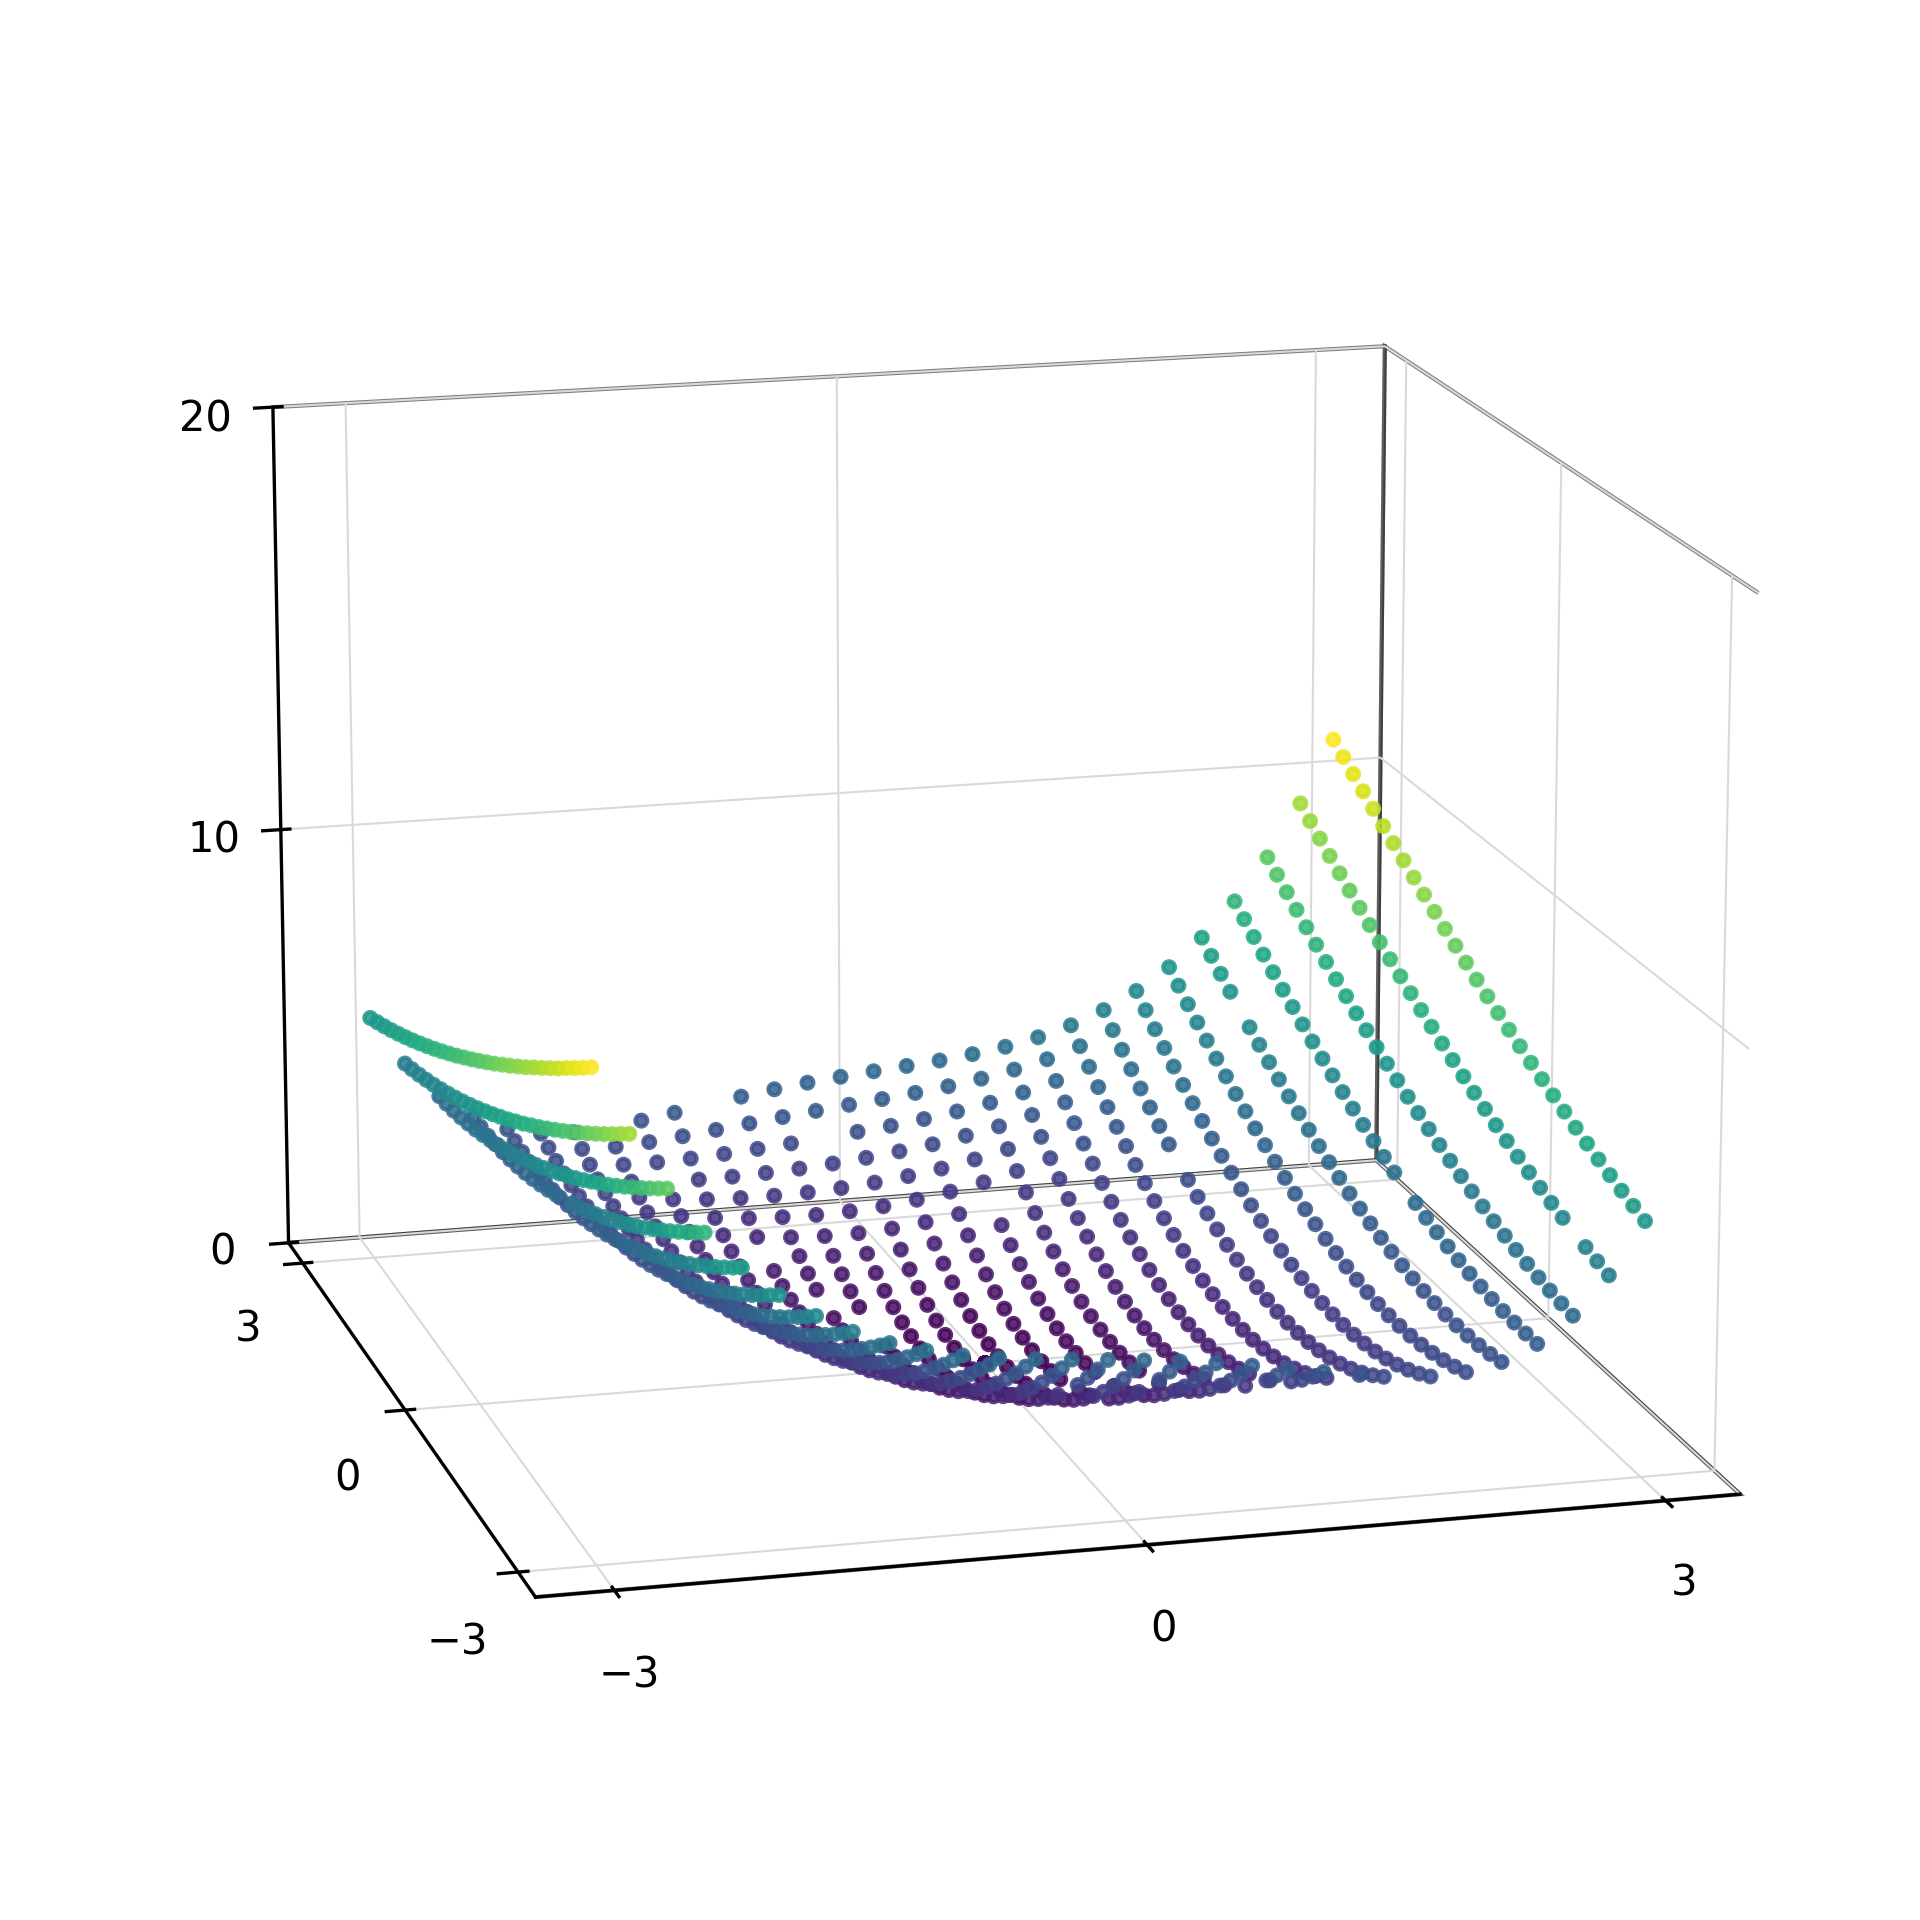
\includegraphics[width=0.48\textwidth]{plot/v.png}
\hfill
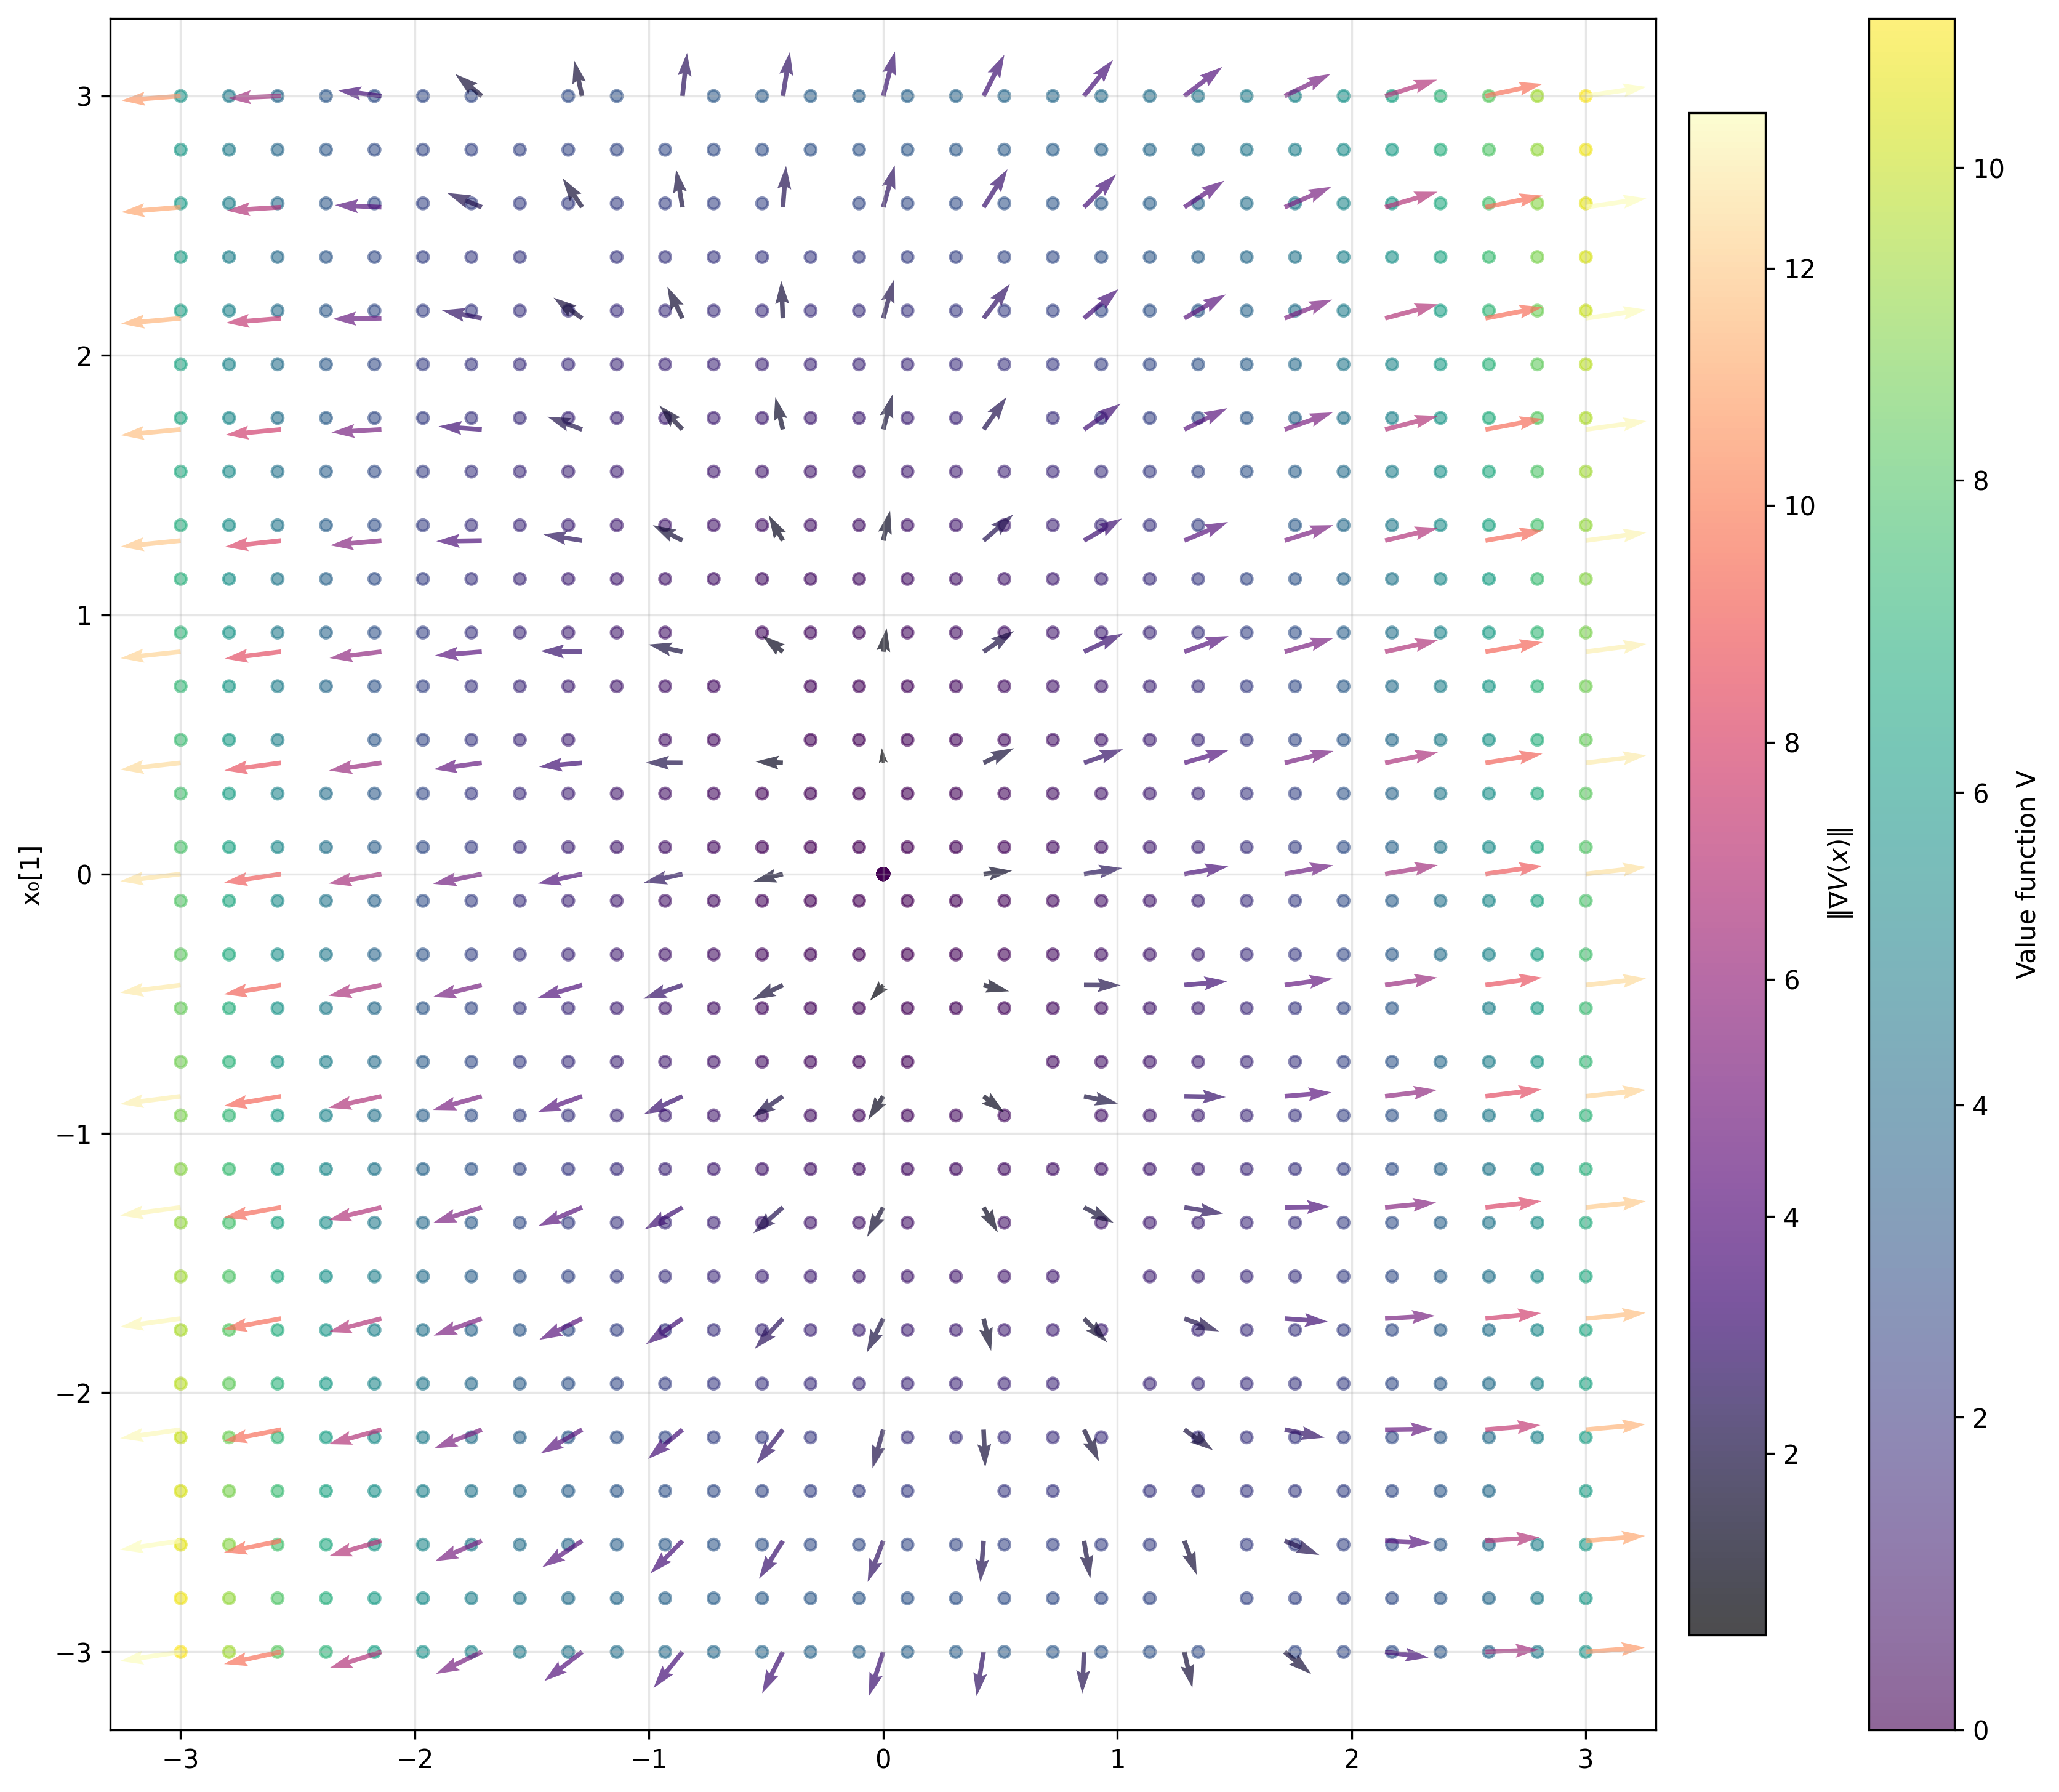
\includegraphics[width=0.48\textwidth]{plot/dv.png}
\caption{Left: value function $V(x)$ over $[-3,3]^2$. Right: $V(x)$ (dot color) and $\nabla V(x)$ (arrows); arrow color indicates $\|\nabla V(x)\|$.}
\label{fig:vdp_data}
\end{figure}

We solve the open-loop problem on a $30 \times 30$ grid over $[-3,3]^2$ ($K = 900$ data points).
All experiments run 10 outer iterations, inserting up to 50 neurons per iteration and pruning neurons with $|c| < 10^{-5}$.

%% ---------------------------------------------------------------
\subsubsection{Algorithm~\ref{alg:log}: $\phi_{\log,\gamma}$-penalty with different activation functions}
%% ---------------------------------------------------------------

First we train the model with the Algorithem \ref{alg:log}. 
We sweep over different activation function and hypeparameter groups and observe the effect on the validation error. 

Table~\ref{tab:alg1_gradient} isolates the effect of gradient augmentation ($L^2$ loss, value only, vs.\ $H^1$ loss, value + gradient) on the validation error. 

\begin{table}[H]
\centering
\caption{Effect of gradient training on validation error ($\alpha = 10^{-5}$, $\gamma = 1$).}
\label{tab:alg1_gradient}
\begin{subtable}{0.48\textwidth}
\centering
\setlength{\tabcolsep}{12pt}
\renewcommand{\arraystretch}{1.25}
\begin{tabular}{lcc}
\toprule
Activation & $L^2$ trained & $H^1$ trained \\
\midrule
softplus & $8.61\text{e-}2$ & $5.19\text{e-}1$ \\
tanh & $3.59\text{e-}2$ & $4.76\text{e-}1$ \\
Gaussian & $3.05\text{e-}2$ & $4.16\text{e-}1$ \\
\bottomrule
\end{tabular}
\caption{Effect of gradient training on $\mathrm{Err}_{L^2}$ }
\label{tab:alg1_gradient_errl2}
\end{subtable}
\hfill
\begin{subtable}{0.48\textwidth}
\centering
\setlength{\tabcolsep}{12pt}
\renewcommand{\arraystretch}{1.25}
\begin{tabular}{lcc}
\toprule
Activation & $L^2$ trained & $H^1$ trained \\
\midrule
softplus & $5.63\text{e-}1$ & $2.92\text{e-}1$ \\
tanh & $4.68\text{e-}1$ & $3.14\text{e-}1$ \\
Gaussian & $4.64\text{e-}1$ & $9.94\text{e-}2$ \\
\bottomrule
\end{tabular}
\caption{Effect of gradient training on $\mathrm{Err}_{H^1}$}
\label{tab:alg1_gradient_errh1}
\end{subtable}
\end{table}

\paragraph{\textbf{Choice of Activation Function in Gradient Training.}}
We choose 3 classes of activation functions: ReLU-like (softplus), sigmoidal (tanh-form), and the Gaussian. 
As observed in Table \ref{tab:alg1_gradient}, the Gaussian activation achieves in general the best precision among the 3.
Overall, All three capture the smooth bowl; they differ in how many neurons it takes. 

\begin{figure}[H]
\centering
\captionsetup[subfigure]{justification=centering}
\begin{subfigure}[t]{0.32\textwidth}
\centering
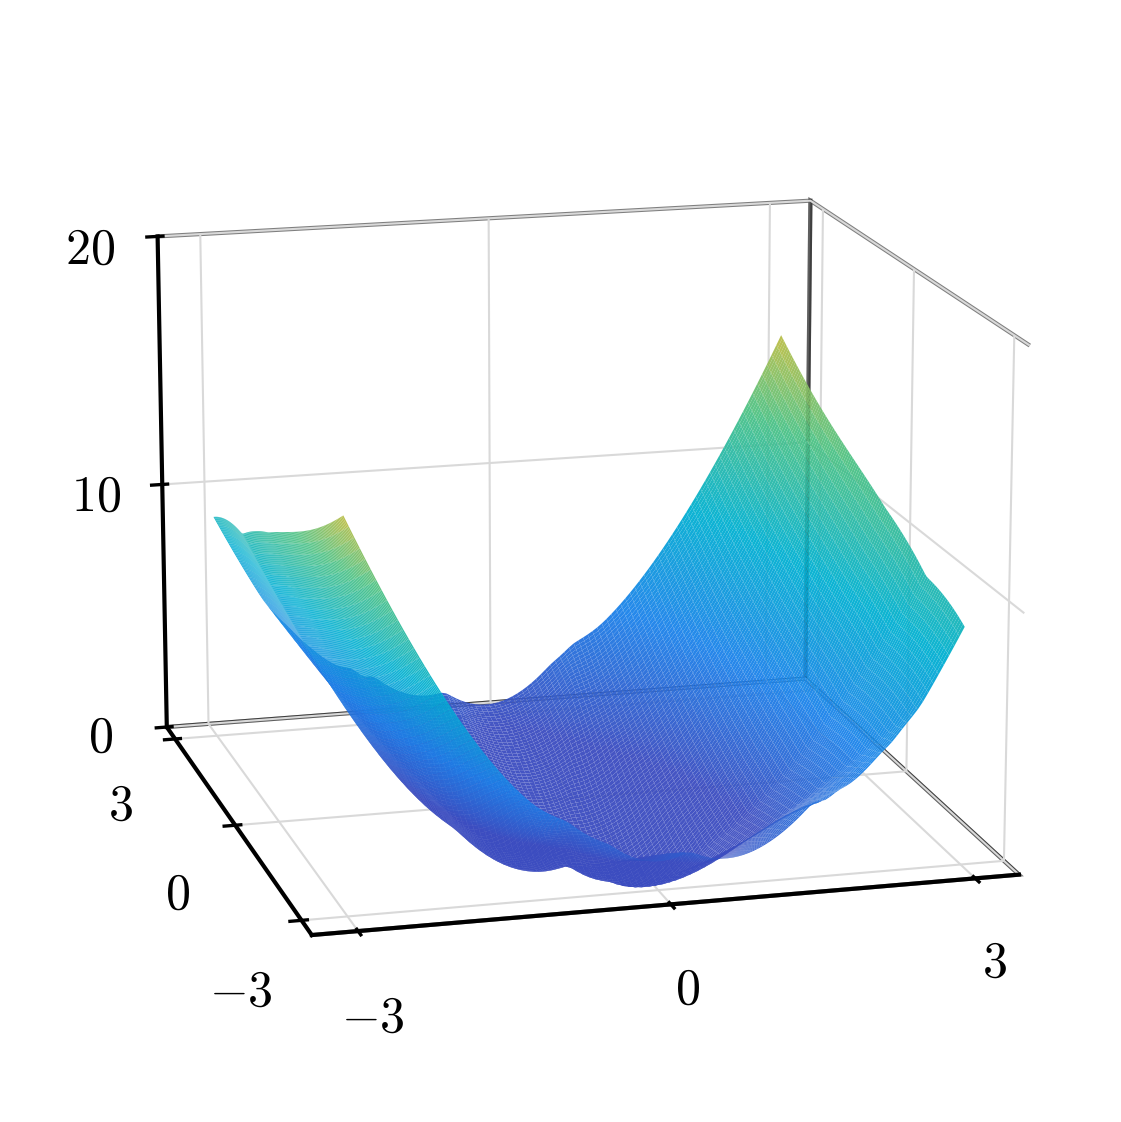
\includegraphics[width=\textwidth]{plot/value_surface_softplus.png}
\caption{softplus\\ ($N=27$, $\mathrm{Err}_{H^1} = 0.29$).}
\label{fig:h1_activation_softplus}
\end{subfigure}
\hfill
\begin{subfigure}[t]{0.32\textwidth}
\centering
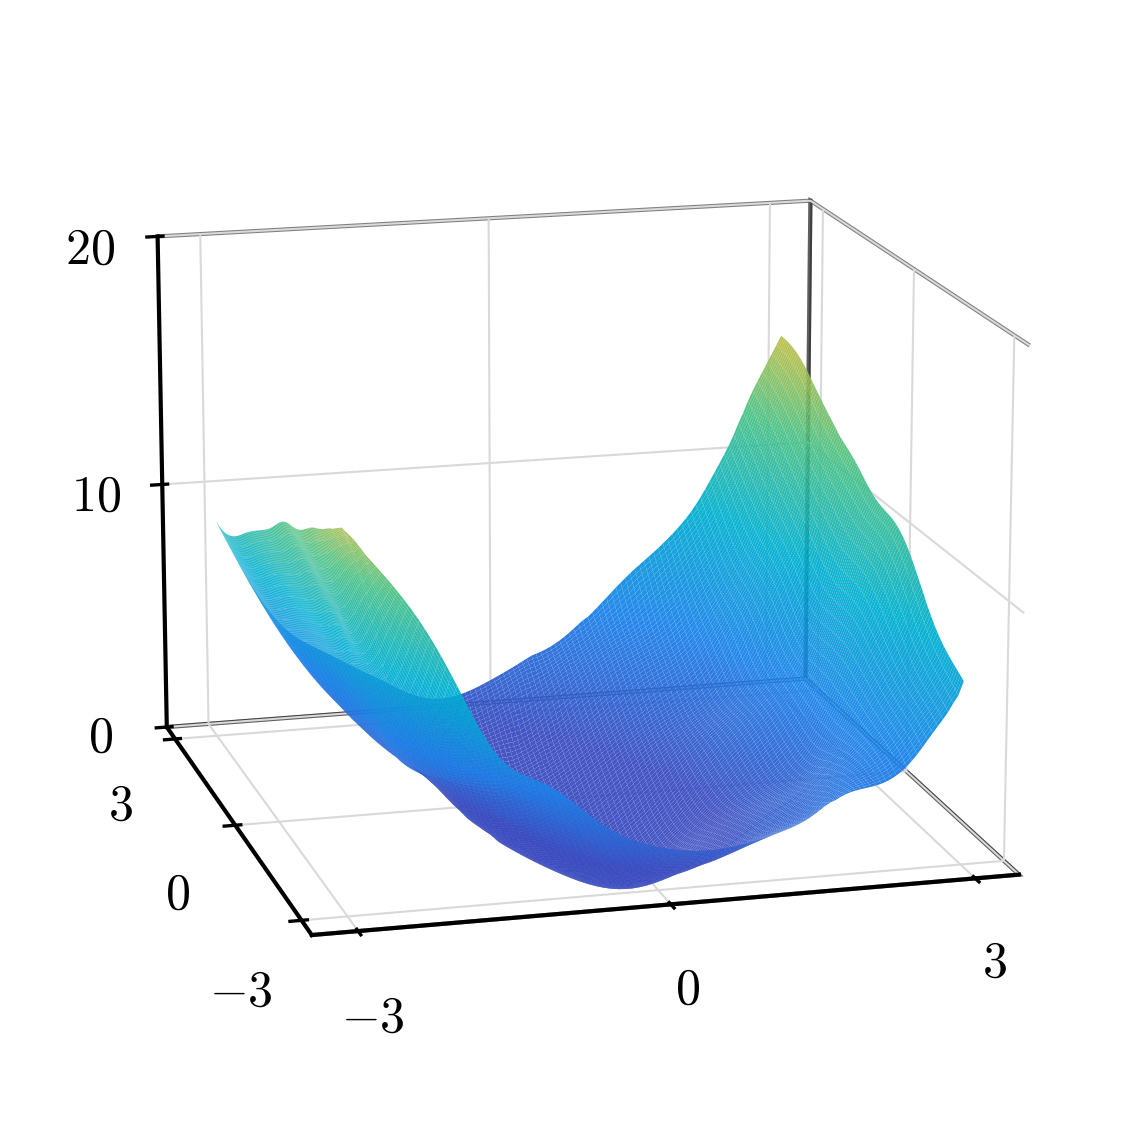
\includegraphics[width=\textwidth]{plot/value_surface_tanh.png}
\caption{tanh\\ ($N=66$, $\mathrm{Err}_{H^1} = 0.31$).}
\label{fig:h1_activation_tanh}
\end{subfigure}
\hfill
\begin{subfigure}[t]{0.32\textwidth}
\centering
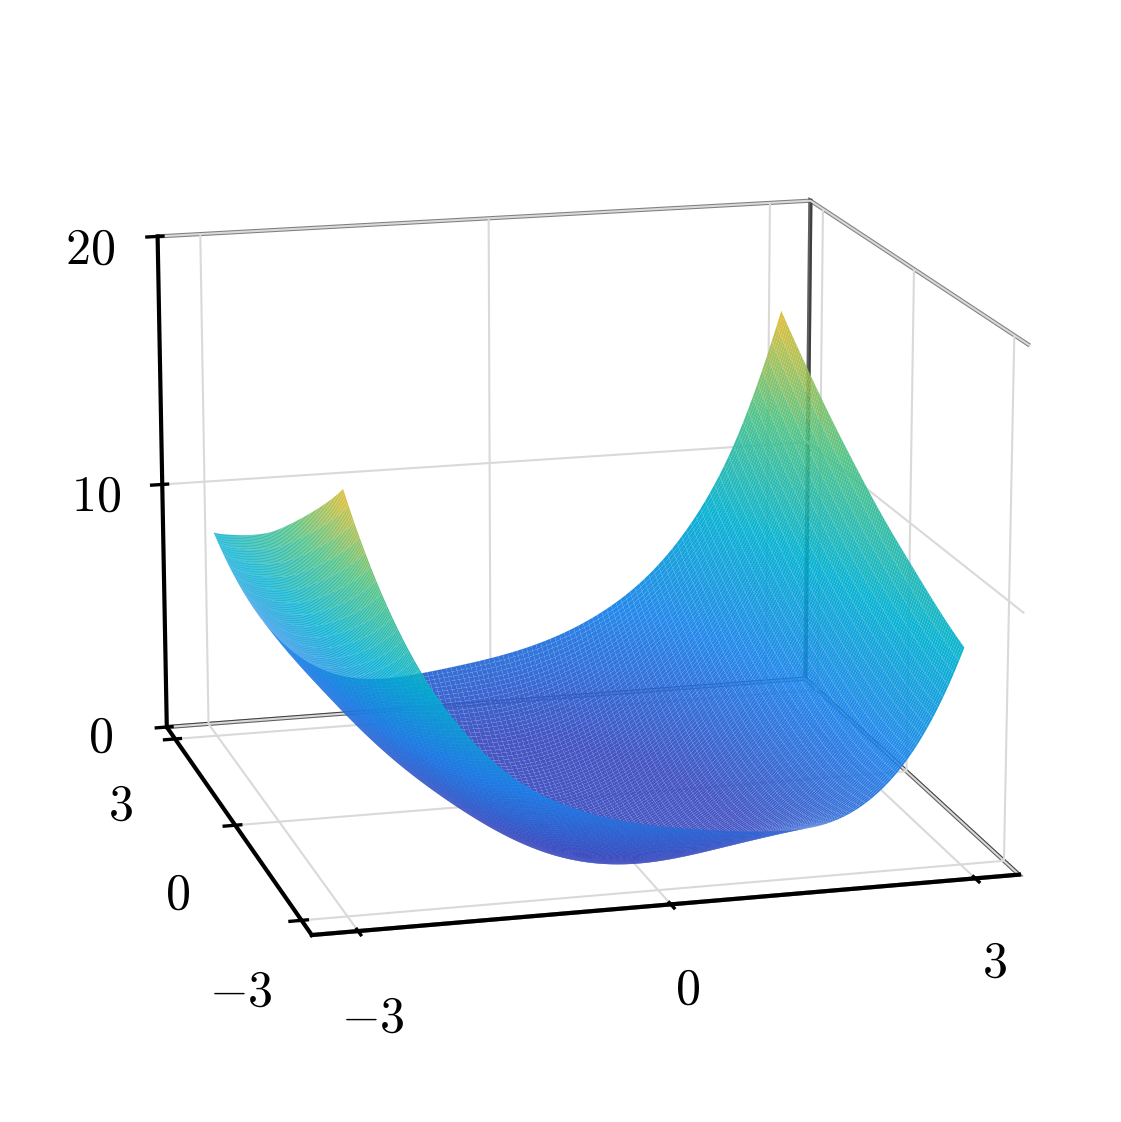
\includegraphics[width=\textwidth]{plot/value_surface_gaussian.png}
\caption{Gaussian\\ ($N=113$, $\mathrm{Err}_{H^1} = 0.10$).}
\label{fig:h1_activation_gaussian}
\end{subfigure}
\caption{Learned value function under the $H^1$ loss for the signed model at the fixed operating point $\gamma = 1$, $\alpha = 10^{-5}$ . All three capture the smooth bowl; they differ in how many neurons it takes.}
\label{fig:h1_activation}
\end{figure}

Tanh saturates for large $|z|$, causing vanishing gradients.
Softplus grows linearly and avoids saturation.
The Gaussian is localized with exponential decay and has a sign-changing derivative $\sigma'(z) = -2z\,e^{-z^2}$ (a bump that is accurate where it sits but must be tiled densely to cover a smooth field).

\begin{table}[H]
\centering
\caption{Network size (sparsity) for each activation, paired with the validation error natural to each loss ($\mathrm{Err}_{L^2}$ for the $L^2$ loss, $\mathrm{Err}_{H^1}$ for the $H^1$ loss; $\alpha = 10^{-5}$, $\gamma = 1$).}
\label{tab:alg1_sparsity}
\begin{subtable}{0.48\textwidth}
\centering
\setlength{\tabcolsep}{12pt}
\renewcommand{\arraystretch}{1.25}
\begin{tabular}{lcc}
\toprule
Activation & $N$ & $\mathrm{Err}_{L^2}$ \\
\midrule
softplus & 58 & $8.61\text{e-}2$ \\
tanh & 75 & $3.59\text{e-}2$ \\
Gaussian & 105 & $3.05\text{e-}2$ \\
\bottomrule
\end{tabular}
\caption{$L^2$ trained}
\label{tab:alg1_sparsity_l2}
\end{subtable}
\hfill
\begin{subtable}{0.48\textwidth}
\centering
\setlength{\tabcolsep}{12pt}
\renewcommand{\arraystretch}{1.25}
\begin{tabular}{lcc}
\toprule
Activation & $N$ & $\mathrm{Err}_{H^1}$ \\
\midrule
softplus & 27 & $2.92\text{e-}1$ \\
tanh & 66 & $3.14\text{e-}1$ \\
Gaussian & 113 & $9.94\text{e-}2$ \\
\bottomrule
\end{tabular}
\caption{$H^1$ trained}
\label{tab:alg1_sparsity_h1}
\end{subtable}
\end{table}

With the $H^1$ loss, $\mathrm{Err}_{H^1}$ drops dramatically for the Gaussian ($9.94 \times 10^{-2}$), whose localized sign-changing derivative reconstructs the smooth gradient field most accurately, while tanh ($3.14 \times 10^{-1}$) and softplus ($2.92 \times 10^{-1}$) improve more modestly. 
This accuracy is not free: the Gaussian pays with the largest neuron count ($N = 113$), whereas softplus matches tanh's $\mathrm{Err}_{H^1}$ ($2.92 \times 10^{-1}$ vs.\ $3.14 \times 10^{-1}$) with far fewer neurons ($27$ vs.\ $66$). On this smooth target the choice of smooth activation trades sparsity against gradient accuracy rather than fit viability.

The performance differences across activations can be understood from two angles: approximation capability and sparsity.

\paragraph{\textbf{Mass Saturation of Derivative near 0 deteriorate the approximation.}}
The gradient kernel column for neuron~$n$ at data point~$x_m$ is $\sigma'(a_n \cdot x_m + b_n) \cdot a_n$; the diversity of these columns determines how well the network can fit the gradient field.
The distribution of $\sigma'(z)$ across all (neuron, data point) pairs indicates the mass saturation near zero:

\begin{figure}[H]
\centering
\captionsetup[subfigure]{justification=centering}
\begin{subfigure}[t]{0.32\textwidth}
\centering
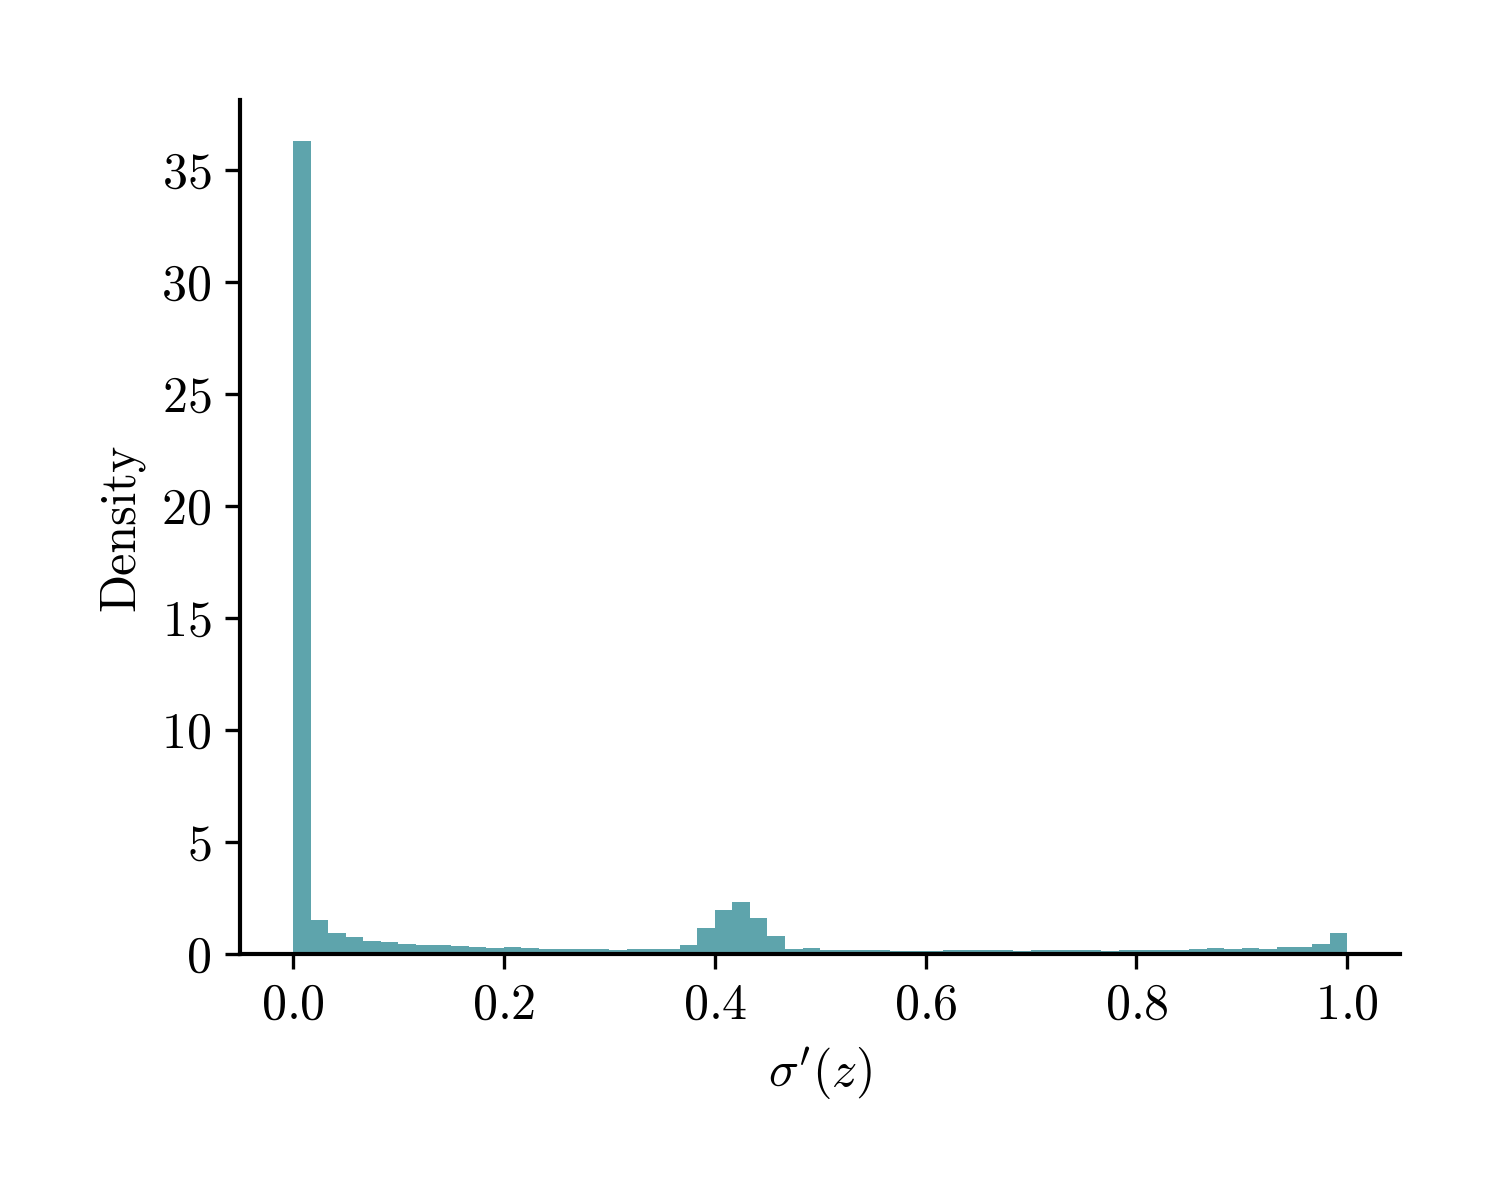
\includegraphics[width=\textwidth]{plot/derivative_distribution_tanh.png}
\caption{tanh, $N=66$ \\ ($65\%$ with $|\sigma'| < 0.05$).}
\label{fig:deriv_tanh}
\end{subfigure}
\hfill
\begin{subfigure}[t]{0.32\textwidth}
\centering
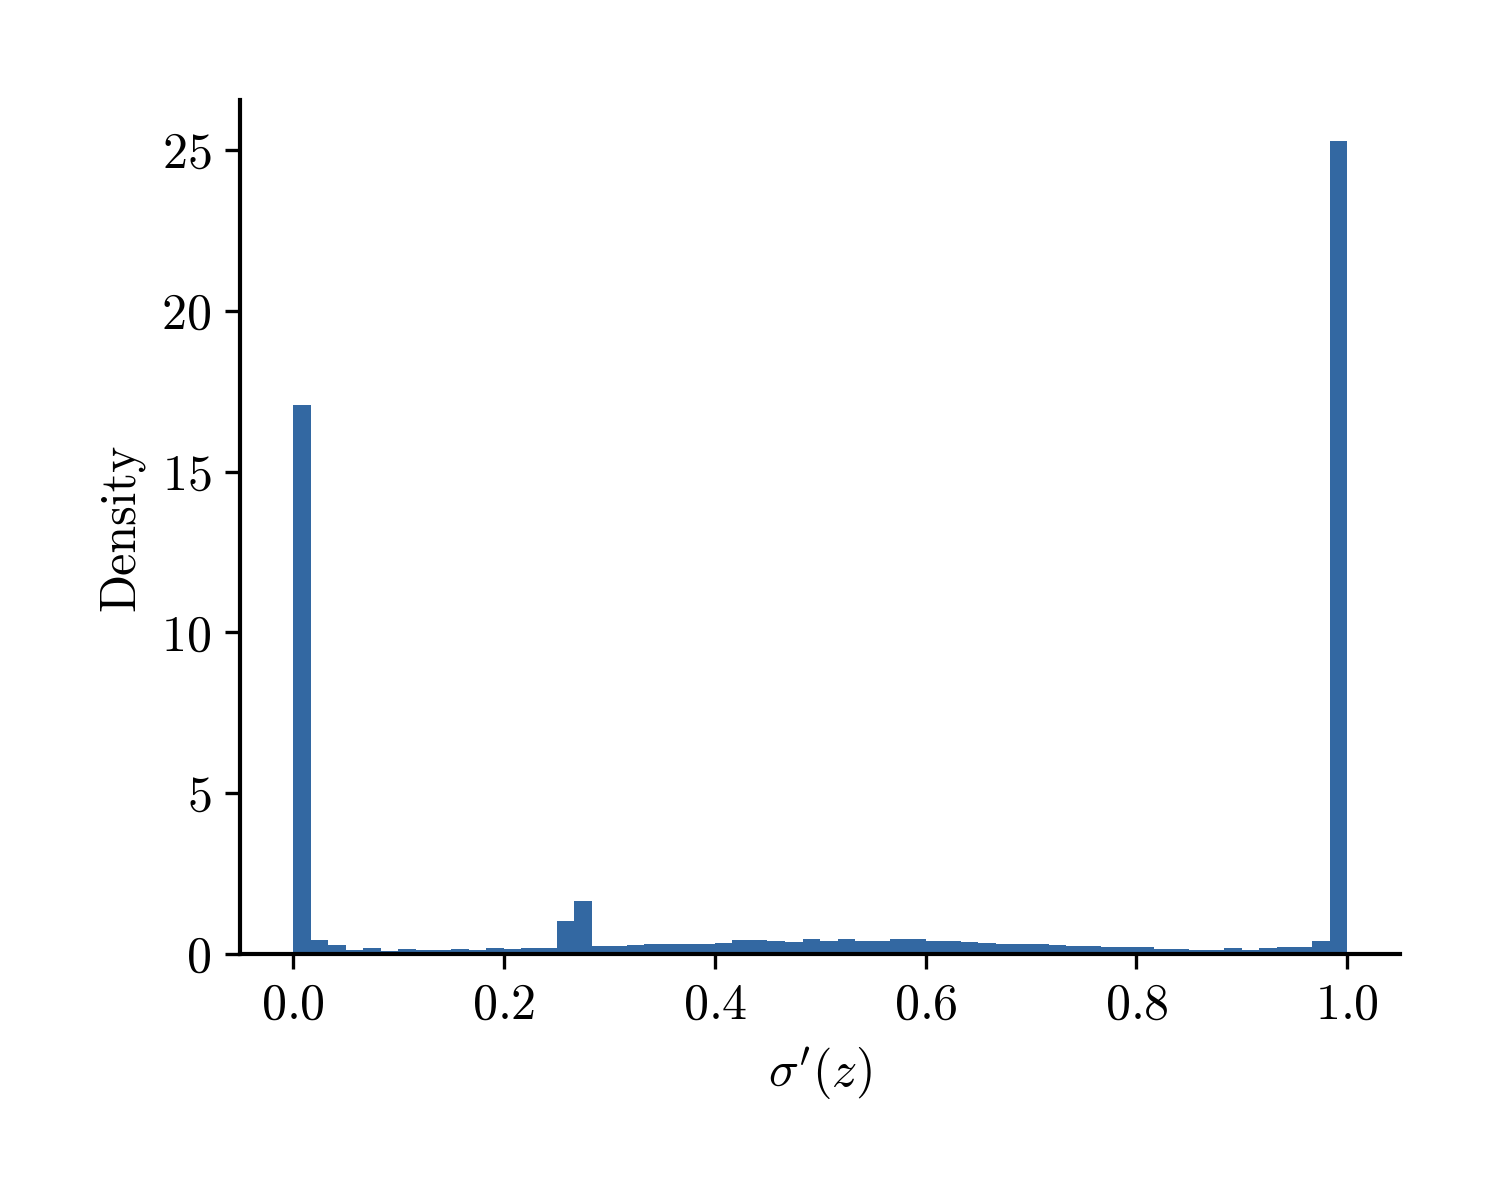
\includegraphics[width=\textwidth]{plot/derivative_distribution_softplus.png}
\caption{softplus, $N=27$ \\ ($30\%$ with $|\sigma'| < 0.05$).}
\label{fig:deriv_softplus}
\end{subfigure}
\hfill
\begin{subfigure}[t]{0.32\textwidth}
\centering
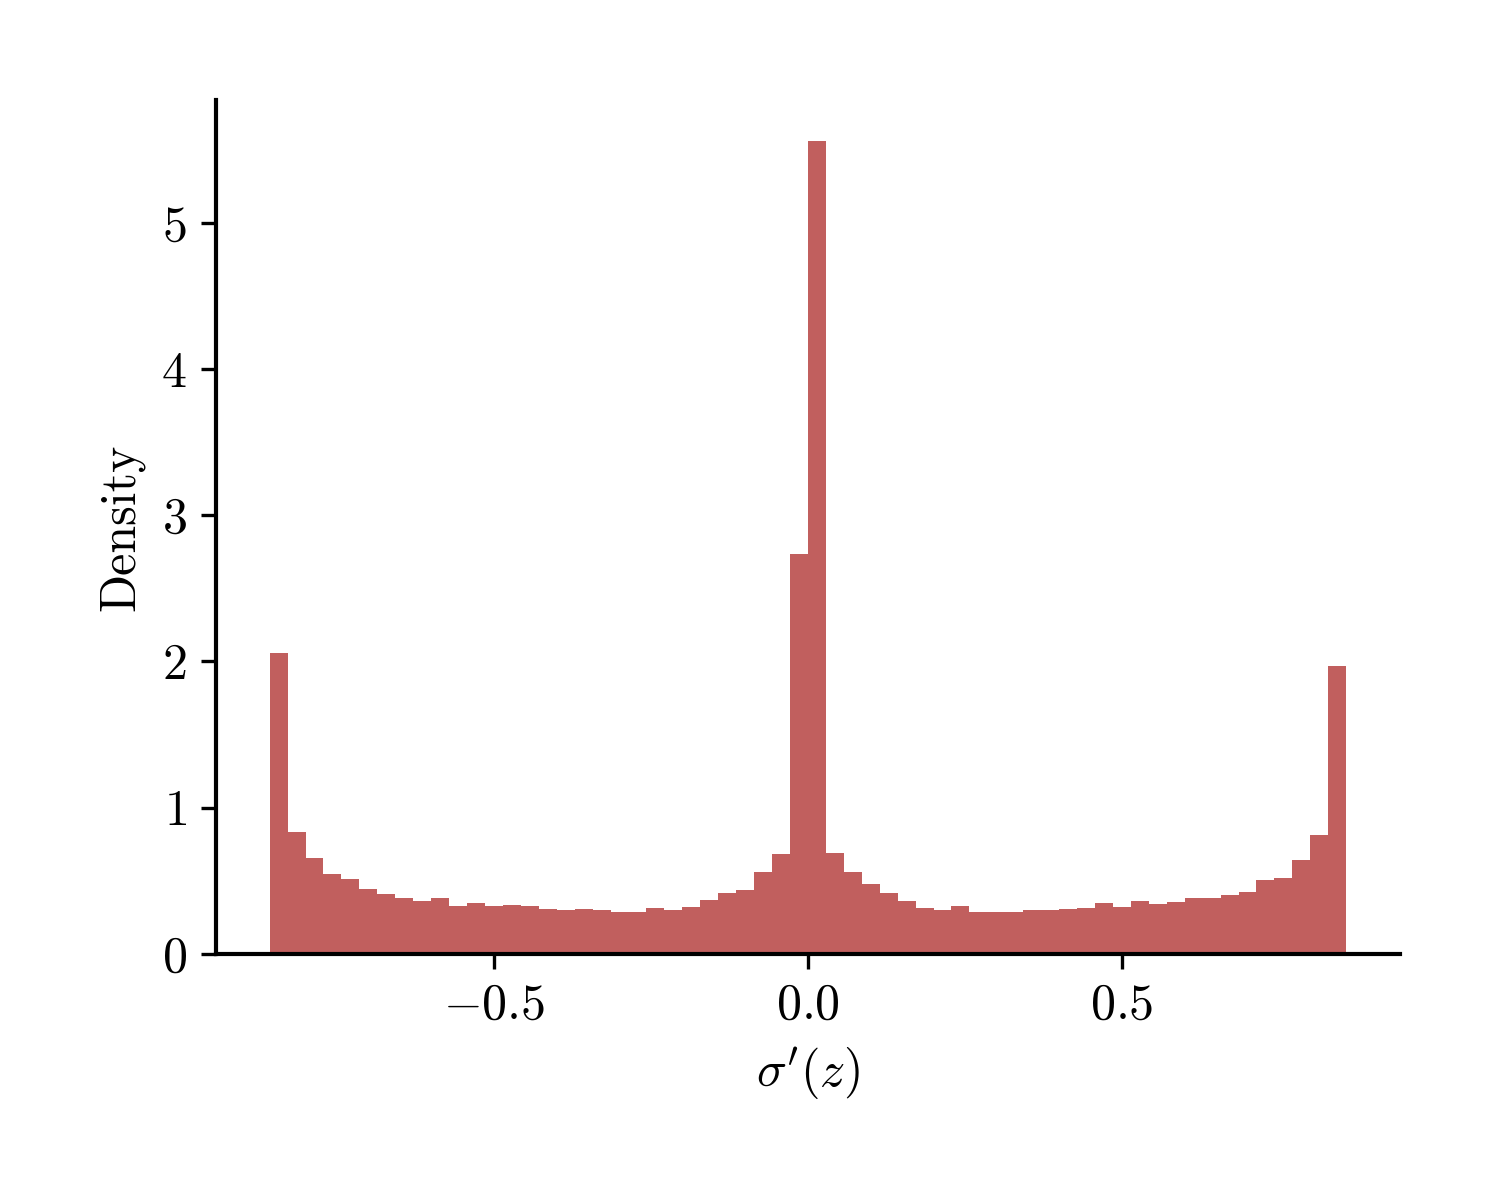
\includegraphics[width=\textwidth]{plot/derivative_distribution_gaussian.png}
\caption{Gaussian, $N=113$ \\ ($27\%$ with $|\sigma'| < 0.05$).}
\label{fig:deriv_gaussian}
\end{subfigure}
\caption{Distribution of $\sigma'(z)$ across all (neuron, data point) pairs for the signed $H^1$ model at the fixed operating point ($\gamma = 1$, $\alpha = 10^{-5}$). The percentage is the fraction of derivative values with $|\sigma'| < 0.05$.}
\label{fig:derivative_distribution}
\end{figure}

The bottleneck for tanh is that two-sided saturation makes many gradient kernel columns redundant, so a given gradient accuracy costs more neurons rather than being unattainable; the Gaussian's sign-changing derivative is the most expressive per neuron but the least sparse.

\paragraph{\textbf{Multiple local maximum of dual profile hurts sparsity.}}
The Gaussian and softplus fits differ sharply in size: 113 neurons versus 27, a factor of~$4.2$, even though the Gaussian is the more accurate of the two ($\mathrm{Err}_{H^1} = 9.9 \times 10^{-2}$ vs.\ $2.9 \times 10^{-1}$).
Table~\ref{tab:insertion_diag} tracks the two fits neuron-by-neuron.
The full objective $J = L(\mu) + \alpha\,\Phi(\mu)$ decreases at every iteration for both, confirming that the inserted neurons are genuine descent directions.
But the Gaussian adds them in large batches (7--15 per iteration) whereas softplus adds only 1--5, and the descent per neuron differs accordingly: each Gaussian neuron lowers~$J$ by $\sim 10^{-4}$ (down to $2 \times 10^{-5}$ by the final iteration), while a softplus neuron typically lowers it by $10^{-3}$--$10^{-2}$.

\begin{table}[H]
\centering
\setlength{\tabcolsep}{10pt}
\renewcommand{\arraystretch}{1.2}
\caption{Per-iteration insertion diagnostics for the Gaussian and softplus $H^1$ fits ($\alpha = 10^{-5}$, $\gamma = 1$).}
\label{tab:insertion_diag}
\begin{tabular}{ccccccc}
\toprule
 & \multicolumn{3}{c}{Gaussian} & \multicolumn{3}{c}{Softplus} \\
\cmidrule(lr){2-4} \cmidrule(lr){5-7}
Iter & $N$ & Ins & $\Delta J / n$ & $N$ & Ins & $\Delta J / n$ \\
\midrule
1  & 7   & 7  & ---                & 2  & 2 & ---                \\
2  & 14  & 7  & $2.8 \times 10^{-3}$ & 3  & 1 & $1.7 \times 10^{-1}$ \\
3  & 24  & 10 & $5.6 \times 10^{-4}$ & 6  & 3 & $5.2 \times 10^{-3}$ \\
4  & 34  & 10 & $1.0 \times 10^{-4}$ & 8  & 2 & $3.6 \times 10^{-3}$ \\
5  & 42  & 8  & $1.8 \times 10^{-4}$ & 11 & 3 & $1.9 \times 10^{-2}$ \\
6  & 57  & 15 & $5.9 \times 10^{-5}$ & 13 & 2 & $1.1 \times 10^{-3}$ \\
7  & 72  & 15 & $1.6 \times 10^{-4}$ & 15 & 2 & $1.2 \times 10^{-3}$ \\
8  & 86  & 14 & $2.2 \times 10^{-4}$ & 18 & 3 & $1.4 \times 10^{-3}$ \\
9  & 99  & 13 & $6.6 \times 10^{-5}$ & 22 & 4 & $2.8 \times 10^{-4}$ \\
10 & 113 & 14 & $2.0 \times 10^{-5}$ & 27 & 5 & $9.3 \times 10^{-4}$ \\
\midrule
Total & 113 & & & 27 & & \\
\bottomrule
\end{tabular}
\\[6pt]
{\small
\raggedright
$N$ = support size after SSN and pruning;\;
\textit{Ins} = neurons added that iteration;\;
$\Delta J / n$ = decrease of the objective $J = L(\mu) + \alpha\,\Phi(\mu)$ per neuron added, relative to the previous iterate (iteration~1 has no predecessor).\par}
\end{table}

The difference reflects how many descent directions the dictionary offers at each step, governed by the dual variable $p_t(\omega) = \langle \sigma(\cdot\,;\omega),\, g_t \rangle$, where $g_t$ is the current residual.
The Gaussian activation is localized: $\sigma(x;\omega)$ is a bump concentrated near the hyperplane $\{x : a \cdot x + b \approx 0\}$, so $p_t(\omega)$ is sensitive to local residual structure, and even small residual pockets push $|p_t(\omega)| > \alpha$ for many~$\omega$.
The insertion step therefore finds a fresh batch of admissible atoms every iteration, each correcting only a small local portion of the residual.
Softplus has global support, so $p_t(\omega)$ averages the residual over the entire domain---positive and negative contributions cancel, fewer~$\omega$ exceed the threshold~$\alpha$, but each admitted atom removes a global component of the residual.

In conclusion:
\begin{itemize}
	\item Gaussian yields the best gradient accuracy ($\mathrm{Err}_{H^1} = 9.9 \times 10^{-2}$) but uses 113~neurons. Its localized activation offers many shallow descent directions, so the algorithm keeps inserting neurons with diminishing per-neuron returns.
	\item Softplus reaches moderate gradient accuracy ($\mathrm{Err}_{H^1} = 2.9 \times 10^{-1}$) with only 27~neurons---the sparsest fit. Each neuron removes a global component of the residual, so the dual variable drops below~$\alpha$ after few insertions.
	\item Tanh is dominated: 66~neurons for $\mathrm{Err}_{H^1} = 3.1 \times 10^{-1}$---essentially softplus's accuracy at more than twice the neuron count---because its two-sided saturation yields a narrow, mostly-dead derivative that wastes atoms without improving the gradient fit.
\end{itemize}



\paragraph{\textbf{Effect of $\alpha$ and $\gamma$.}}
Table~\ref{tab:alg1_alpha} shows the effect of the nonconvex correction $\gamma$ at $\alpha = 10^{-5}$, $H^1$ loss.
The nonconvex penalty helps the two activations differently.
For softplus, raising $\gamma$ to $10$ cuts the $H^1$ error nearly in half (from $3.35 \times 10^{-1}$ at $\gamma = 0$ to $1.76 \times 10^{-1}$) at a comparable neuron count.
For the Gaussian, the same sweep barely moves the already-low error (${\approx}\,1.0 \times 10^{-1}$) while the neuron count grows ($91 \to 119$): the localized activation is insensitive to the penalty's nonconvexity, whereas the broad softplus ridge benefits from the sharper thresholding.

Table~\ref{tab:alg1_alpha} sweeps $\alpha$ for $\gamma = 0$ (pure $\ell^1$) and $\gamma = 10$ (strong nonconvex correction) across the two activations.
Smaller $\alpha$ increases accuracy at the cost of more neurons for both.
The nonconvex correction sharpens this frontier most for softplus---at $\alpha = 10^{-4}$ it halves the $H^1$ error ($3.24 \times 10^{-1} \to 1.68 \times 10^{-1}$) at a similar neuron count---while for the Gaussian it yields only a modest gain.

\begin{table}[H]
\centering
\caption{Algorithm~1: effect of $\alpha$ with $\gamma = 0$ vs.\ $\gamma = 10$ ($H^1$ loss).}
\label{tab:alg1_alpha}
\begin{subtable}{0.48\textwidth}
\centering
\setlength{\tabcolsep}{8pt}
\renewcommand{\arraystretch}{1.2}
\begin{tabular}{ccccc}
\toprule
 & \multicolumn{2}{c}{$\gamma = 0$} & \multicolumn{2}{c}{$\gamma = 10$} \\
\cmidrule(lr){2-3} \cmidrule(lr){4-5}
$\alpha$ & $N$ & $\mathrm{Err}_{H^1}$ & $N$ & $\mathrm{Err}_{H^1}$ \\
\midrule
$10^{-2}$ & 14 & $3.57 \times 10^{-1}$ & 10 & $3.78 \times 10^{-1}$ \\
$10^{-3}$ & 15 & $3.43 \times 10^{-1}$ & 14 & $2.79 \times 10^{-1}$ \\
$10^{-4}$ & 20 & $3.24 \times 10^{-1}$ & 25 & $1.68 \times 10^{-1}$ \\
$10^{-5}$ & 21 & $3.35 \times 10^{-1}$ & 23 & $1.76 \times 10^{-1}$ \\
\bottomrule
\end{tabular}
\caption{Softplus}
\label{tab:alg1_alpha_softplus}
\end{subtable}
\hfill
\begin{subtable}{0.48\textwidth}
\centering
\setlength{\tabcolsep}{8pt}
\renewcommand{\arraystretch}{1.2}
\begin{tabular}{ccccc}
\toprule
 & \multicolumn{2}{c}{$\gamma = 0$} & \multicolumn{2}{c}{$\gamma = 10$} \\
\cmidrule(lr){2-3} \cmidrule(lr){4-5}
$\alpha$ & $N$ & $\mathrm{Err}_{H^1}$ & $N$ & $\mathrm{Err}_{H^1}$ \\
\midrule
$10^{-2}$ & 12 & $2.31 \times 10^{-1}$ & 19 & $2.06 \times 10^{-1}$ \\
$10^{-3}$ & 26 & $1.64 \times 10^{-1}$ & 33 & $1.28 \times 10^{-1}$ \\
$10^{-4}$ & 81 & $1.08 \times 10^{-1}$ & 80 & $1.02 \times 10^{-1}$ \\
$10^{-5}$ & 91 & $1.03 \times 10^{-1}$ & 119 & $9.88 \times 10^{-2}$ \\
\bottomrule
\end{tabular}
\caption{Gaussian}
\label{tab:alg1_alpha_gaussian}
\end{subtable}
\end{table}


%% ---------------------------------------------------------------
\subsubsection{Algorithm~\ref{alg:q}: $|c|^q$-penalty with $\reluk$ activation}
%% ---------------------------------------------------------------

Algorithm~2 uses the $\reluk$ atom $\sigma(z) = \mathrm{ReLU}(z)^k$ with the pure power penalty $\alpha \sum_i |c_i|^q$, $q = 2/(k+1)$ (i.e.\ $\gamma = 0$. 
The swept knob is the power $k$; all fits below are at the fixed operating point $\alpha = 10^{-5}$.


\begin{figure}[H]
\centering
\captionsetup[subfigure]{justification=centering}
\begin{subfigure}[t]{0.32\textwidth}
\centering

\includegraphics[width=\textwidth]{plot/value_surface_p2.png}
\caption{$k=2$\\ ($N=41$, $\mathrm{Err}_{H^1} = 0.10$).}
\label{fig:H1_power_p2}
\end{subfigure}
\hfill
\begin{subfigure}[t]{0.32\textwidth}
\centering

\includegraphics[width=\textwidth]{plot/value_surface_p3.png}
\caption{$k=3$\\ ($N=20$, $\mathrm{Err}_{H^1} = 0.10$).}
\label{fig:H1_power_p3}
\end{subfigure}
\hfill
\begin{subfigure}[t]{0.32\textwidth}
\centering
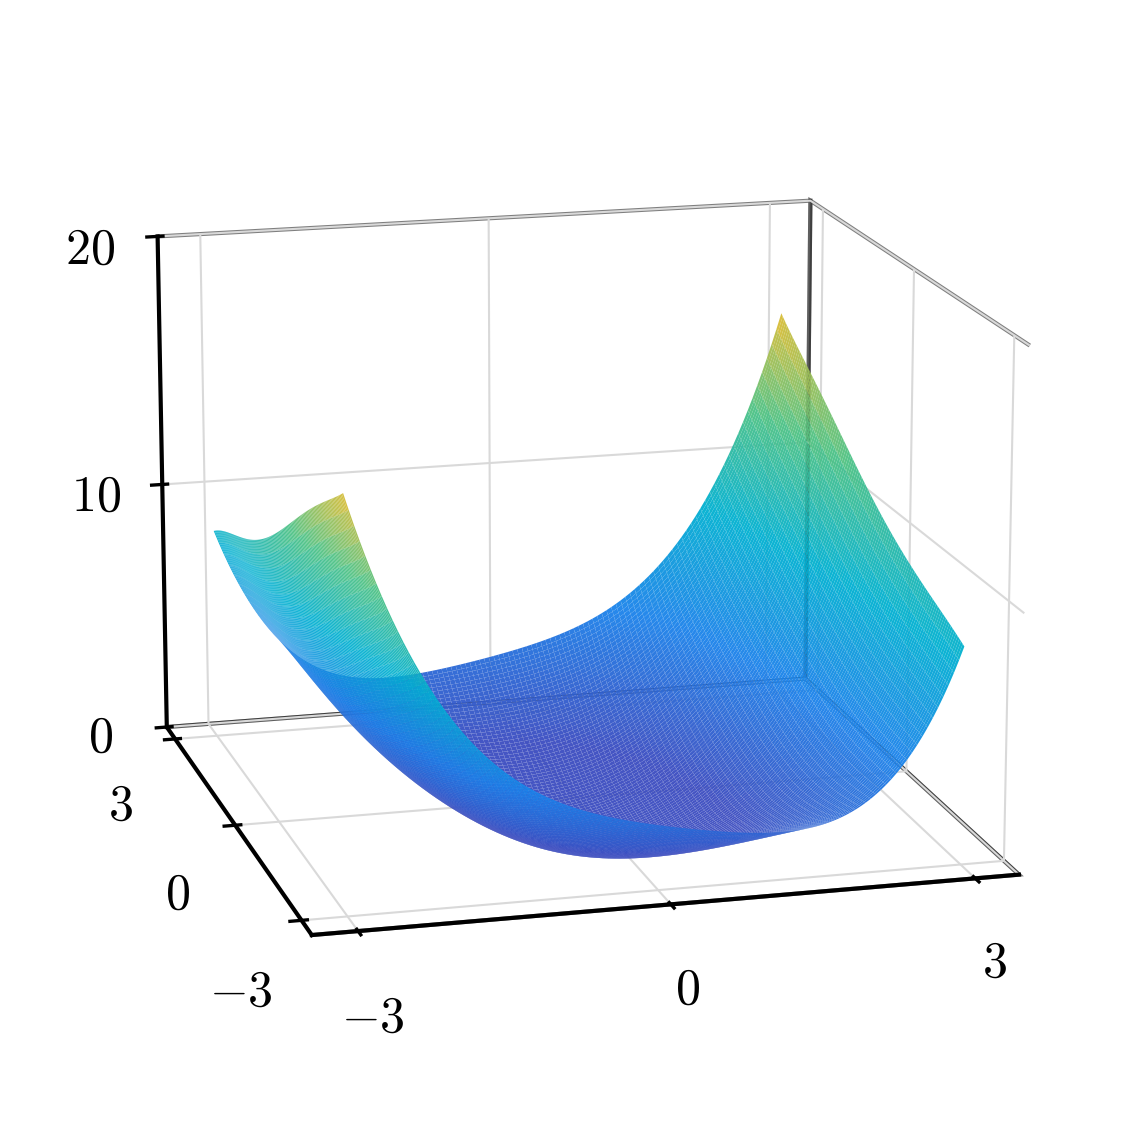
\includegraphics[width=\textwidth]{plot/value_surface_p5.png}
\caption{$k=5$\\ ($N=21$, $\mathrm{Err}_{H^1} = 0.10$).}
\label{fig:H1_power_p5}
\end{subfigure}
\caption{$H^1$-trained model with $\alpha = 10^{-5}$, for the representative powers $k \in \{2, 3, 5\}$. All reconstruct the smooth bowl; they differ only in neuron count.}
\label{fig:H1_power}
\end{figure}

Under the $L^2$ loss the gradient error stays large for every power ($\mathrm{Err}_{H^1} \approx 4$--$5 \times 10^{-1}$): the value-only fit ignores $\nabla V$, so the atoms are placed without regard to the gradient field.
The $H^1$ loss drives the gradient error down to $\approx 1.0 \times 10^{-1}$ for \emph{all} powers (Table~\ref{tab:alg2_gradient}).
Gradient augmentation is decisive and uniform in $k$: the fit becomes gradient-accurate regardless of the atom power.

\begin{table}[H]
\centering
\caption{Algorithm~2: network size and validation error vs.\ the atom power $k$ ($\alpha = 10^{-5}$).}
\label{tab:alg2_gradient}
\begin{subtable}{0.48\textwidth}
\centering
\setlength{\tabcolsep}{6pt}
\renewcommand{\arraystretch}{1.25}
\begin{tabular}{lccc}
\toprule
Power & $N$ & $\mathrm{Err}_{L^2}$ & $\mathrm{Err}_{H^1}$ \\
\midrule
$k = 2$ & 14 & $5.05 \times 10^{-2}$ & $4.83 \times 10^{-1}$ \\
$k = 2.01$ & 14 & $4.83 \times 10^{-2}$ & $4.81 \times 10^{-1}$ \\
$k = 3$ & 12 & $5.98 \times 10^{-2}$ & $4.94 \times 10^{-1}$ \\
$k = 4$ & 12 & $5.48 \times 10^{-2}$ & $4.61 \times 10^{-1}$ \\
$k = 5$ & 10 & $4.77 \times 10^{-2}$ & $4.04 \times 10^{-1}$ \\
\bottomrule
\end{tabular}
\caption{$L^2$ trained}
\label{tab:alg2_gradient_l2}
\end{subtable}
\hfill
\begin{subtable}{0.48\textwidth}
\centering
\setlength{\tabcolsep}{6pt}
\renewcommand{\arraystretch}{1.25}
\begin{tabular}{lccc}
\toprule
Power & $N$ & $\mathrm{Err}_{L^2}$ & $\mathrm{Err}_{H^1}$ \\
\midrule
$k = 2$ & 41 & $4.16 \times 10^{-1}$ & $9.84 \times 10^{-2}$ \\
$k = 2.01$ & 42 & $4.17 \times 10^{-1}$ & $9.93 \times 10^{-2}$ \\
$k = 3$ & 20 & $4.17 \times 10^{-1}$ & $1.00 \times 10^{-1}$ \\
$k = 4$ & 22 & $4.16 \times 10^{-1}$ & $9.97 \times 10^{-2}$ \\
$k = 5$ & 21 & $4.14 \times 10^{-1}$ & $1.04 \times 10^{-1}$ \\
\bottomrule
\end{tabular}
\caption{$H^1$ trained}
\label{tab:alg2_gradient_h1}
\end{subtable}
\end{table}

Under the $H^1$ loss the gradient accuracy is essentially flat in $k$ ($\mathrm{Err}_{H^1} \approx 1.0 \times 10^{-1}$ for every power), while the neuron count falls sharply as the power grows: $k = 2$ needs $41$ atoms, whereas $k = 3$, $k = 4$ and $k = 5$ need only about $20$ (Table~\ref{tab:alg2_gradient}\,(b)).
Raising the power buys sparsity for free: the exponent $q = 2/(k+1)$ shrinks, the coefficient penalty $|c|^q$ becomes more concave, and the more aggressive selection keeps the same accuracy with fewer atoms---a smooth value function lies in the span of a few high-power atoms.
The trend is monotone in $k$, with no intermediate ``sweet spot'' and no high-power breakdown.
Under the $L^2$ loss the fits are uniformly sparse ($10$--$14$ atoms) but gradient-blind ($\mathrm{Err}_{H^1} \approx 4$--$5 \times 10^{-1}$, Table~\ref{tab:alg2_gradient}\,(a)).



%% ---------------------------------------------------------------
\subsubsection{Summary}
%% ---------------------------------------------------------------

Figure~\ref{fig:summary_frontier} plots insertion growth trajectory --- the best relative $H^1$ error reached with a given number of neurons. 
Algorithm~2 dominates: $\reluk$ at $k = 5$ and $k = 2$ reach the best gradient accuracy ($\mathrm{Err}_{H^1} \approx 1.0 \times 10^{-1}$) with only $\approx 20$--$40$ neurons, whereas the most accurate Algorithm-1 activation, the Gaussian, needs $113$ neurons for the same accuracy, and softplus/tanh plateau at a coarser error. 
At equal gradient accuracy Algorithm~2 uses a fraction of the atoms.
\begin{figure}[H]
\centering

\includegraphics[width=0.8\textwidth]{plot/frontier.png}
\caption{Running best relative $H^1$ validation error vs.\ network size ($\alpha = 10^{-5}$).}
\label{fig:summary_frontier}
\end{figure}

We synthesise the optimal feedback law from $y_0 = (2, 1)$. 
Figure~\ref{fig:summary_feedback} shows $\|y(t)\|$ and $|u(t)|$ for softplus, the Gaussian, and $\reluk$ ($k = 5$), beside the true optimal control. 
All three drive the state to the origin and track the true control, at essentially the true optimal closed-loop cost ($6.68$, $6.51$, $6.49$ vs.\ $6.48$). 
\begin{figure}[H]
\centering
\captionsetup[subfigure]{justification=centering}
\begin{subfigure}[t]{0.48\textwidth}
\centering

\includegraphics[width=\textwidth]{plot/feedback_state.png}
\caption{State norm $\|y(t)\|$.}
\label{fig:summary_feedback_state}
\end{subfigure}
\hfill
\begin{subfigure}[t]{0.48\textwidth}
\centering

\includegraphics[width=\textwidth]{plot/feedback_control.png}
\caption{Control $|u(t)|$.}
\label{fig:summary_feedback_control}
\end{subfigure}
\caption{Evoluation of the state and control from $y_0 = (2, 1)$ under the feedback synthesised from each fitted value function, beside the true optimal control.}
\label{fig:summary_feedback}
\end{figure}

Figure~\ref{fig:summary_weights_raw} shows where the inner weights sit for the Gaussian, softplus, and $\reluk$ ($k = 5$).
The two algorithms produce structurally different representations: Algorithm~2 constrains its atoms to the unit sphere $\mathbb{S}^2$, while Algorithm~1 leaves them free --- the Gaussian atoms in particular span a wide range of norms. 
\begin{figure}[H]
\centering
\captionsetup[subfigure]{justification=centering}
\begin{subfigure}[t]{0.32\textwidth}
\centering

\includegraphics[width=\textwidth]{plot/weights_raw3d_gaussian.png}
\caption{$e^{-x^2} + \alpha\,\phi_1$.}
\end{subfigure}
\hfill
\begin{subfigure}[t]{0.32\textwidth}
\centering

\includegraphics[width=\textwidth]{plot/weights_raw3d_softplus.png}
\caption{$\mathrm{softplus} + \alpha\,\phi_1$.}
\end{subfigure}
\hfill
\begin{subfigure}[t]{0.32\textwidth}
\centering
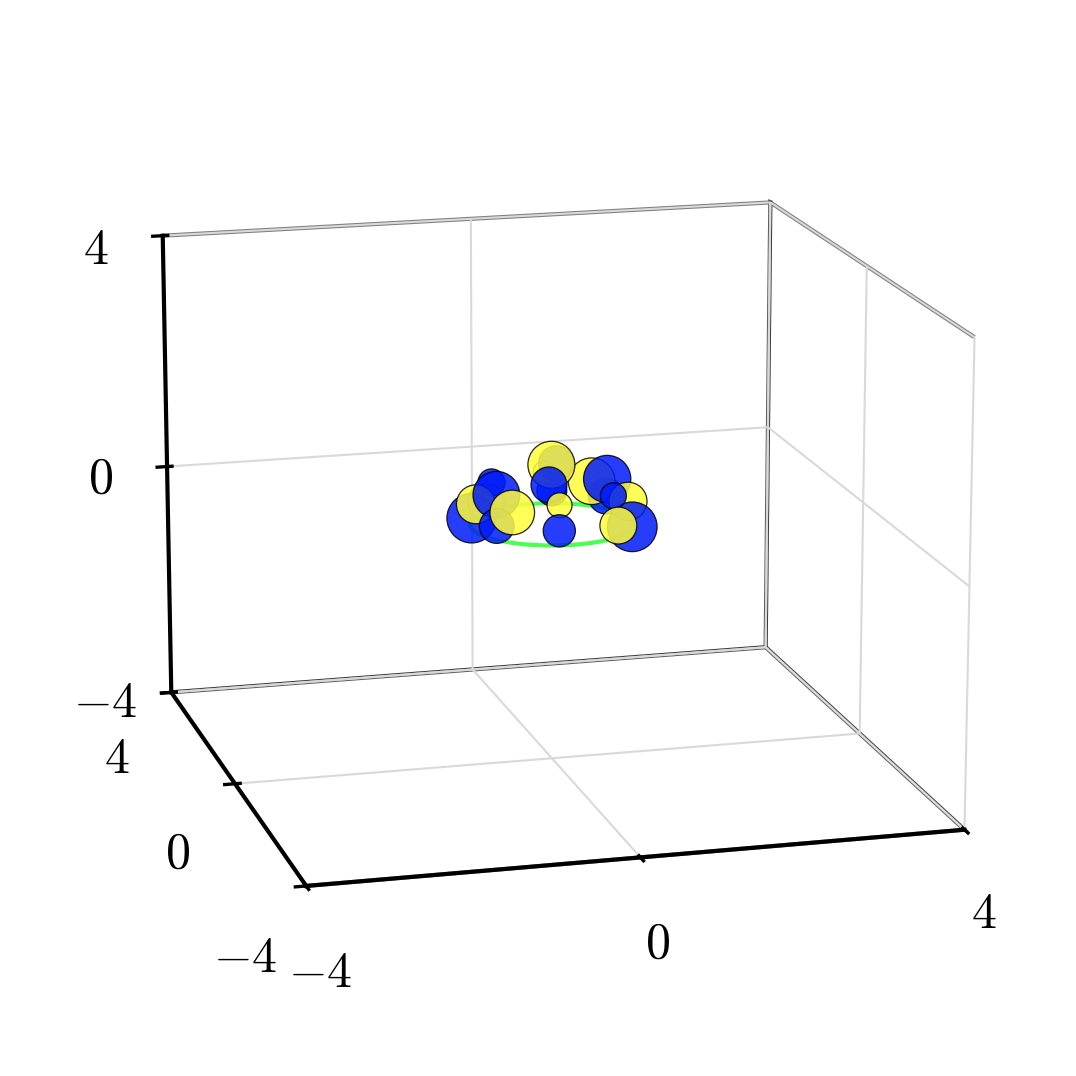
\includegraphics[width=\textwidth]{plot/weights_raw3d_relu5.png}
\caption{$\mathrm{ReLU}^5 + \alpha\,\psi_5$.}
\end{subfigure}
\caption{Inner-weight portrait: raw $(a_1, a_2, b)$ with the unit equator circle (light green, at $b = 0$) for reference ($\alpha = 10^{-5}$). Dot color indicates sign, dot size outer weights magnitute.}
\label{fig:summary_weights_raw}
\end{figure}





\subsection{Pendulum Swing-Up}
We have established that our current network approximate the value function in the Barron space $B_1^k(D)$.
The ability to approximate the discontinuous gradient is potentially limited. 
We now show this with the pendulum example. Moreover, we demonstrate under this limited setting, which model could approximate the discontinuity more effectively.

The example we consider follows from \cite{han2024nonsmooth}.
We write
\begin{equation*}
	x = (x_1,x_2)^T = (\theta,\omega)^T, \qquad \omega=\dot{\theta}.
\end{equation*}
We consider the optimal control problem
\begin{equation*}
	\min_{u \in L^2(0,\infty;\mathbb{R})} \int_0^\infty \big( q_1\sin^2\theta(t) + q_1(\cos\theta(t)-1)^2 + q_2\omega^2(t) + r u^2(t) \big)\,dt
\end{equation*}
subject to
\begin{equation*}
\begin{cases}
	\dot{\theta} = \omega,\\
	\dot{\omega} = -\frac{1}{ml^2}\big(b\omega - mgl\sin\theta - u\big),\\
	(\theta(0),\omega(0))=(x_1,x_2).
\end{cases}
\end{equation*}
The target equilibrium is $x_U=(2j\pi,0)$, $j\in\mathbb{Z}$.

In this setting the state dimension is $d=2$ and the control is scalar.
To initialize the backward integration, we use the local linear-quadratic regulator (LQR) approximation near $x_U$.
Let $\xi=x-x_U$ be the local coordinate around the upright equilibrium.
Linearizing the dynamics at $(x_U,0)$ gives
\begin{equation*}
	\dot{\xi}=A\xi+Bu, \quad A= \begin{pmatrix} 0 & 1\\ \frac{g}{l} & -\frac{b}{ml^2} \end{pmatrix}, \quad B= \begin{pmatrix} 0\\ \frac{1}{ml^2} \end{pmatrix}.
\end{equation*}
The running cost is locally approximated by
\begin{equation*}
	\xi^TQ\xi + r u^2, \qquad Q= \begin{pmatrix} q_1 & 0\\ 0 & q_2 \end{pmatrix}.
\end{equation*}
The local infinite-horizon LQR value function is
\begin{equation*}
	V^\infty(\xi)=\xi^TP\xi,
\end{equation*}
where $P$ is the positive definite solution of the algebraic Riccati equation
\begin{equation*}
	A^TP+PA-\frac{1}{r}PBB^TP+Q=0.
\end{equation*}
The superscript $\infty$ refers to the infinite-horizon LQR problem.
For $\varepsilon>0$, we define the local LQR sublevel set and boundary by
\begin{equation*}
	L_\varepsilon=\{\xi:V^\infty(\xi)\leq \varepsilon\},
	\qquad
	\partial L_\varepsilon=\{\xi:V^\infty(\xi)=\varepsilon\}.
\end{equation*}
The corresponding state-costate system becomes
\begin{equation}
\label{TPBVP_pendulum}
\left\{
\begin{aligned}
	& \dot{\theta}^* = \omega^*,\\
	& \dot{\omega}^* = -\frac{1}{ml^2} \big(b\omega^* - mgl\sin\theta^* - u^*\big),\\
	& -\dot{p}_1^* = 2q_1\sin\theta^* + \frac{g}{l}\cos\theta^*\,p_2^*,\\
	& -\dot{p}_2^* = 2q_2\omega^* + p_1^* - \frac{b}{ml^2}p_2^*,\\
	& x^*(0)=x, \quad x^*(T_x)-x_U\in \partial L_\varepsilon, \quad p^*(T_x)=\nabla V^\infty(x^*(T_x)-x_U).
\end{aligned}
\right.
\end{equation}

In the experiment we use $\varepsilon=2\times 10^{-4}$, and on $\partial L_\varepsilon$ the terminal costate is
\begin{equation*}
	p^*(T_x)=\nabla V^\infty(\xi^*(T_x))=2P\xi^*(T_x).
\end{equation*}
For the data generation, we solve the open-loop PMP system by integrating backward from the local LQR boundary $\partial L_\varepsilon$.
Along each PMP trajectory, the accumulated running cost gives the value sample $V(x)$, and the costate gives the gradient sample $\nabla V(x)=p$.
The backward integration stops when $V$ hits a predefined ceiling. 
This yields the dataset
\begin{equation*}
\{x^m,V(x^m),\nabla V(x^m)\}_{m=1}^M
\end{equation*}

This construction records the nonsmooth geometry of the pendulum value function.
Because the clockwise and counter-clockwise swing-up branches have equal cost at the bottom position $((2k+1)\pi,0)$, the optimal value function is not globally $C^1$.
The generator detects the switching curve by intersecting equal-value contours with their $2\pi$-shifted copies and restricts the PMP trajectories to a consistent smooth branch.
Restriction alone, however, produces \emph{one-sided} data --- every sample stops at the switching curve, so the gradient jump itself would never appear in the training set.
The generator therefore adds an envelope-certified band straddling the switching arms: the raw trajectories are tiled by $\pm 2\pi$ in $\theta$, and a tiled point within the band is kept only if its branch value beats the competing branch's locally extrapolated value, certifying that it carries the true $(V,\nabla V)$ on its side of the curve.
The final $(x,V,dV)$ dataset (3{,}900 samples: a 3{,}000-sample in-basin body plus a 900-sample two-sided band) thus contains the gradient discontinuity as an \emph{interior} feature.
This makes the pendulum benchmark a stress test for the gradient-augmented sparse neural approximation: the value is continuous while its gradient jumps across a switching set that the models see from both sides.
\begin{figure}[H]
\centering
\captionsetup[subfigure]{justification=centering}
\begin{subfigure}[b]{0.32\textwidth}
\centering
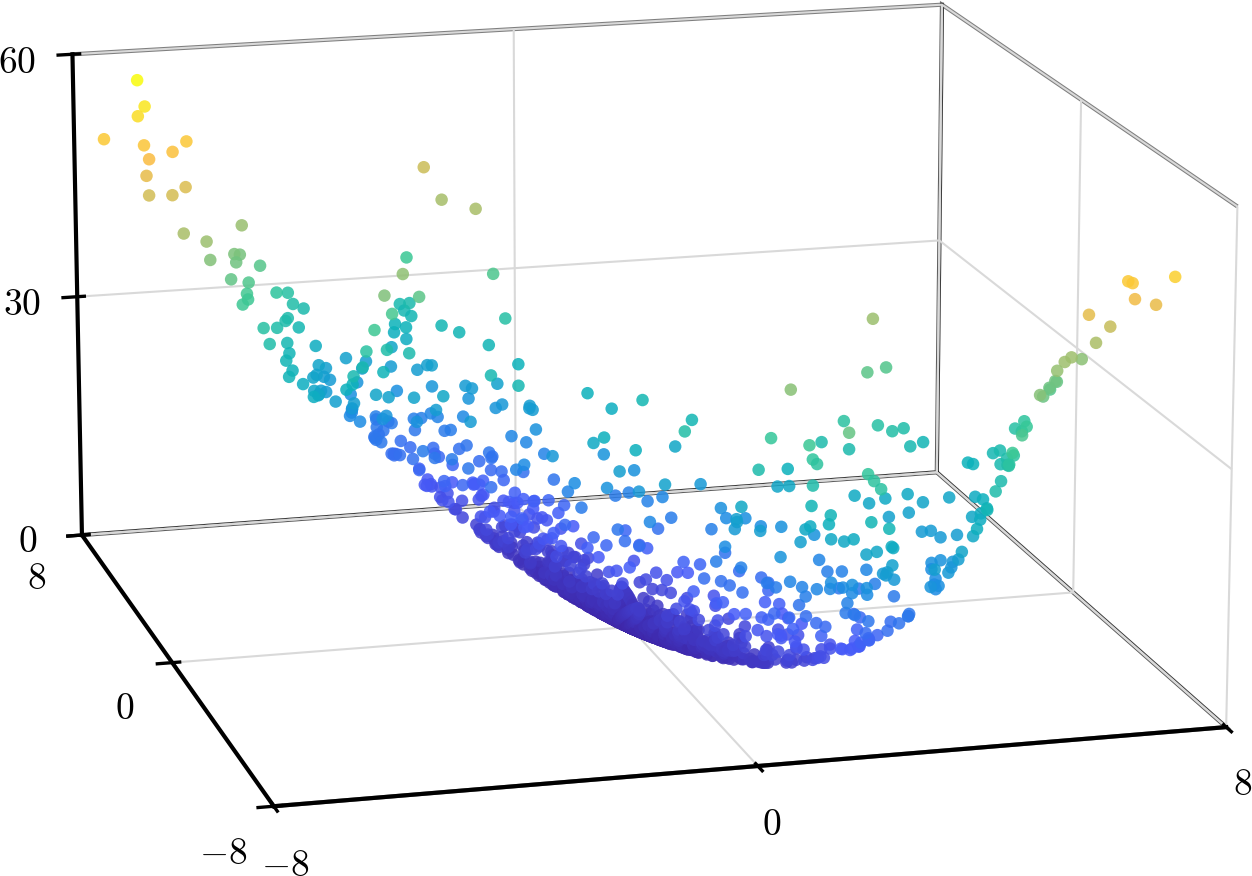
\includegraphics[width=\textwidth]{plot/pendulum_value_scatter.png}
\caption{value samples $\{x^m, V(x^m)\}$.}
\label{fig:pendulum_data_scatter}
\end{subfigure}
\hfill
\begin{subfigure}[b]{0.32\textwidth}
\centering
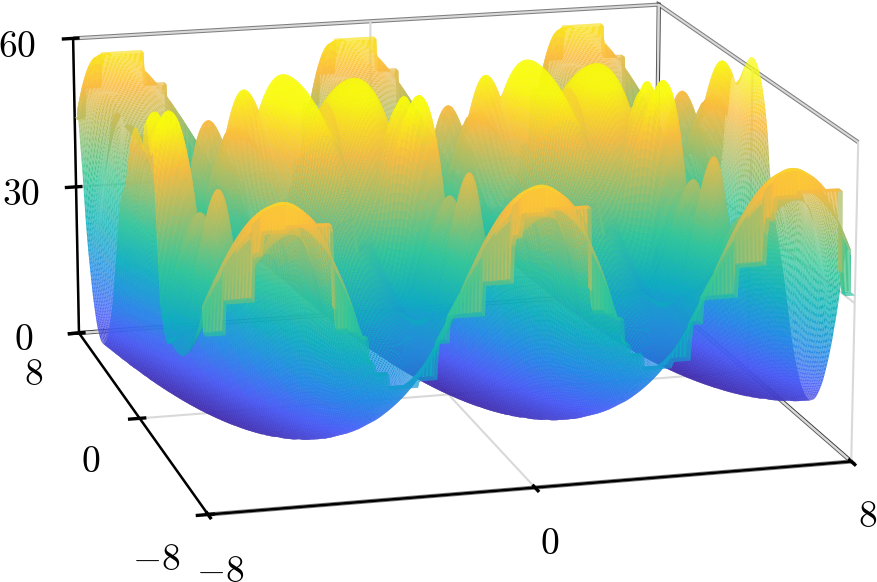
\includegraphics[width=\textwidth]{plot/pendulum_value_surface.png}
\caption{value surface $V(x)$.}
\label{fig:pendulum_data_surface}
\end{subfigure}
\hfill
\begin{subfigure}[b]{0.32\textwidth}
\centering
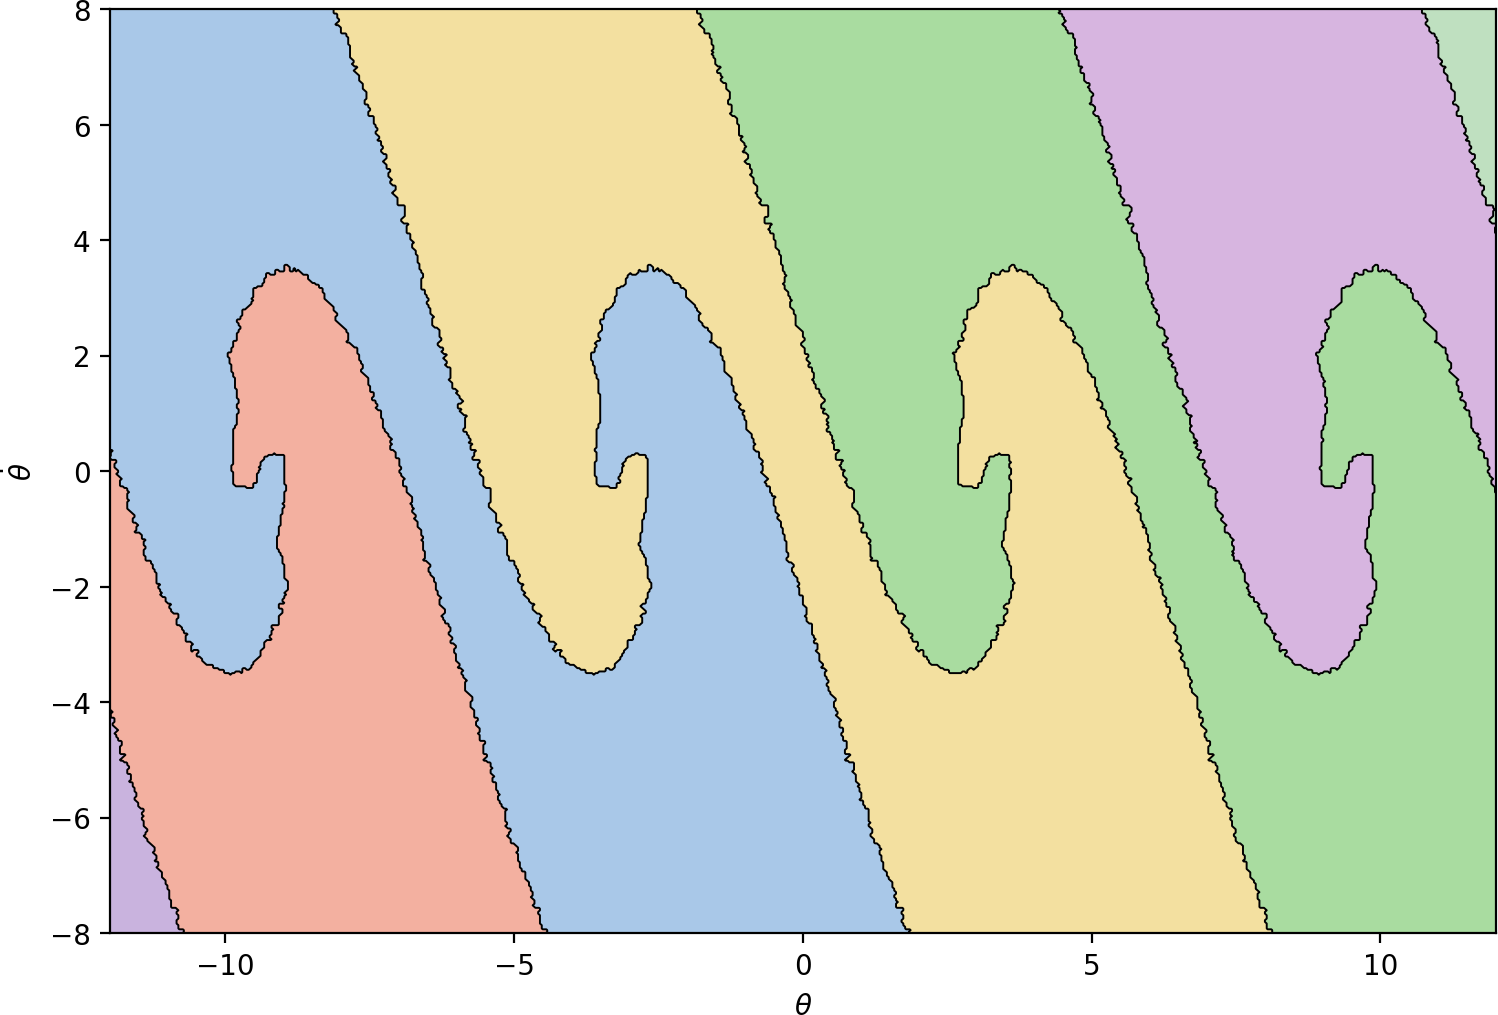
\includegraphics[width=\textwidth]{plot/pendulum_regions.png}
\caption{regions of attraction.}
\label{fig:pendulum_data_regions}
\end{subfigure}
\caption{Optimal value function $V(x)$ over the $(\theta, \dot\theta)$ plane,
$2\pi$-periodic in $\theta$. (a) The raw $(x, V)$ samples produced by the PMP
generator. (b) The reconstructed value surface. (c) Regions of attraction of the
periodic uprights; their boundaries are the switching-set spirals across which 
$\nabla V$ is discontinuous.}
\label{fig:pendulum_data} 
\end{figure}



\subsubsection{Limitation of Fitting the General Value Function}
As in the last example we fit the training data with the models we selected.
Figure~\ref{fig:rs_surfaces} shows the
four fitted surfaces on the same physical window and value range as the true
surface of Figure~\ref{fig:pendulum_data_surface}.
With the two-sided band in the training data the models now shape the full multi-well landscape rather than a single central bowl: $\mathrm{ReLU}^{2}$ raises sharp diagonal walls along the switching arms between the $2k\pi$ wells, the Gaussian reproduces the wells but rounds the ridge off, and softplus smears the structure.
The switching walls are, however, reproduced only approximately --- the quantitative limitation appears on the transect below.

\begin{figure}[H]
\centering
\captionsetup[subfigure]{justification=centering}
\begin{subfigure}[b]{0.24\textwidth}
\centering

\includegraphics[width=\textwidth]{plot/surface_gaussian.png}
\caption{Gaussian + $\phi_{1}$}
\label{fig:rs_surface_gaussian}
\end{subfigure}
\hfill
\begin{subfigure}[b]{0.24\textwidth}
\centering

\includegraphics[width=\textwidth]{plot/surface_softplus.png}
\caption{softplus+ $\phi_{1}$}
\label{fig:rs_surface_softplus}
\end{subfigure}
\hfill
\begin{subfigure}[b]{0.24\textwidth}
\centering

\includegraphics[width=\textwidth]{plot/surface_relu2.png}
\caption{$\mathrm{ReLU}^{2}$+$\phi_2$.}
\label{fig:rs_surface_relu2}
\end{subfigure} 
\hfill
\begin{subfigure}[b]{0.24\textwidth}
\centering

\includegraphics[width=\textwidth]{plot/surface_relu5.png}
\caption{$\mathrm{ReLU}^{5}$+$\phi_5$.}
\label{fig:rs_surface_relu5}
\end{subfigure}
\caption{Learned value surfaces $\hat V(x)$ over the $(\theta,\dot\theta)$
window $[-8,8]^{2}$, displayed on the common range $\hat V\in[0,60]$.
Trained on the two-sided data, the models shape the multi-well landscape;
the sharpness of the switching walls varies with the atom class, from the
crisp $\mathrm{ReLU}^{2}$ ridges to the smeared softplus surface.}
\label{fig:rs_surfaces}
\end{figure}

In Figure~\ref{fig:rs_transect}, a transect along the normal to the
switching curve through the densest data region. The true value (left) is the
continuous lower envelope of the two PMP branches, with a concave kink at the
crossing; the true normal gradient $n\cdot\nabla V$ (right) therefore
\emph{jumps} at the switching set $s=0$.
Unlike the branch-restricted construction, the training data here carry samples
on \emph{both} sides of the curve, so the jump is in-sample --- and the
transect shows that this is necessary but not sufficient. No model reproduces
the jump's magnitude: all of them undershoot the steep pre-jump gradient
(true $n\cdot\nabla V\approx-100$ just before the curve against fitted values
between $-20$ and $-58$), because the finite-width band bounds how much
one-sided steepness the global $H^{1}$ fit will spend neurons on.
$\mathrm{ReLU}^{2}$ comes closest: it is the only model that develops a visible
kink at $s\approx 0$ --- its piecewise-quadratic atoms can break the derivative
across a line --- while the smooth activations necessarily interpolate a gentle
slope through the discontinuity. The near-band error is thus a genuine
representation cost at a \emph{seen} discontinuity, no longer a boundary-layer
artifact of one-sided sampling.

\begin{figure}[H]
\centering
\captionsetup[subfigure]{justification=centering}
\begin{subfigure}[b]{0.48\textwidth}
\centering

\includegraphics[width=\textwidth]{plot/transect_value.png}
\caption{value $V$ along the normal.}
\label{fig:rs_transect_value}
\end{subfigure}
\hfill
\begin{subfigure}[b]{0.48\textwidth}
\centering

\includegraphics[width=\textwidth]{plot/transect_normal_gradient.png}
\caption{normal gradient $n\cdot\nabla V$ along the normal.}
\label{fig:rs_transect_gradient}
\end{subfigure}
\caption{Transect along the switching-set normal, parametrized by signed
distance $s$ (the models saw data on both sides). Left: the true value (dashed)
is a continuous lower envelope with a kink at $s=0$. Right: the true normal
gradient jumps at $s=0$ by ${\approx}100$ units; $\mathrm{ReLU}^{2}$ alone
develops a kink near $s=0$, while the smooth models interpolate through the
discontinuity, and no model reproduces the jump's full magnitude --- a
representation limit at a seen discontinuity.}
\label{fig:rs_transect}
\end{figure}


\subsubsection{The $ReLU^2$ fits the discontinuous gradient}
Despite the limitation of fitting the discontinuous gradient in general, ReLU$^2$ demonstrate better performance in fitting the swtiching profile than other activation function. 

 
Figure~\ref{fig:rs_frontier}
tracks the best relative $H^{1}$ validation error reached as neurons are
inserted, for each activation paired with its penalty. $\mathrm{ReLU}^{2}$
(fractional penalty $\psi_{2}$) separates from the field almost immediately and
reaches the lowest error of all ($\approx 3.6\times10^{-1}$ at 113 neurons);
softplus plateaus near $5.4\times10^{-1}$, and $\mathrm{ReLU}^{5}$ ($\psi_{5}$)
and the Gaussian stall around $5.5$--$5.9\times10^{-1}$. The errors are
uniformly higher than on a smooth target --- the two-sided switching band makes
the fit genuinely harder for every atom class --- but the per-neuron accuracy
advantage of the \emph{low-power} rectified atom is unambiguous; raising the
power to $5$ forfeits it.

\begin{figure}[H]
\centering
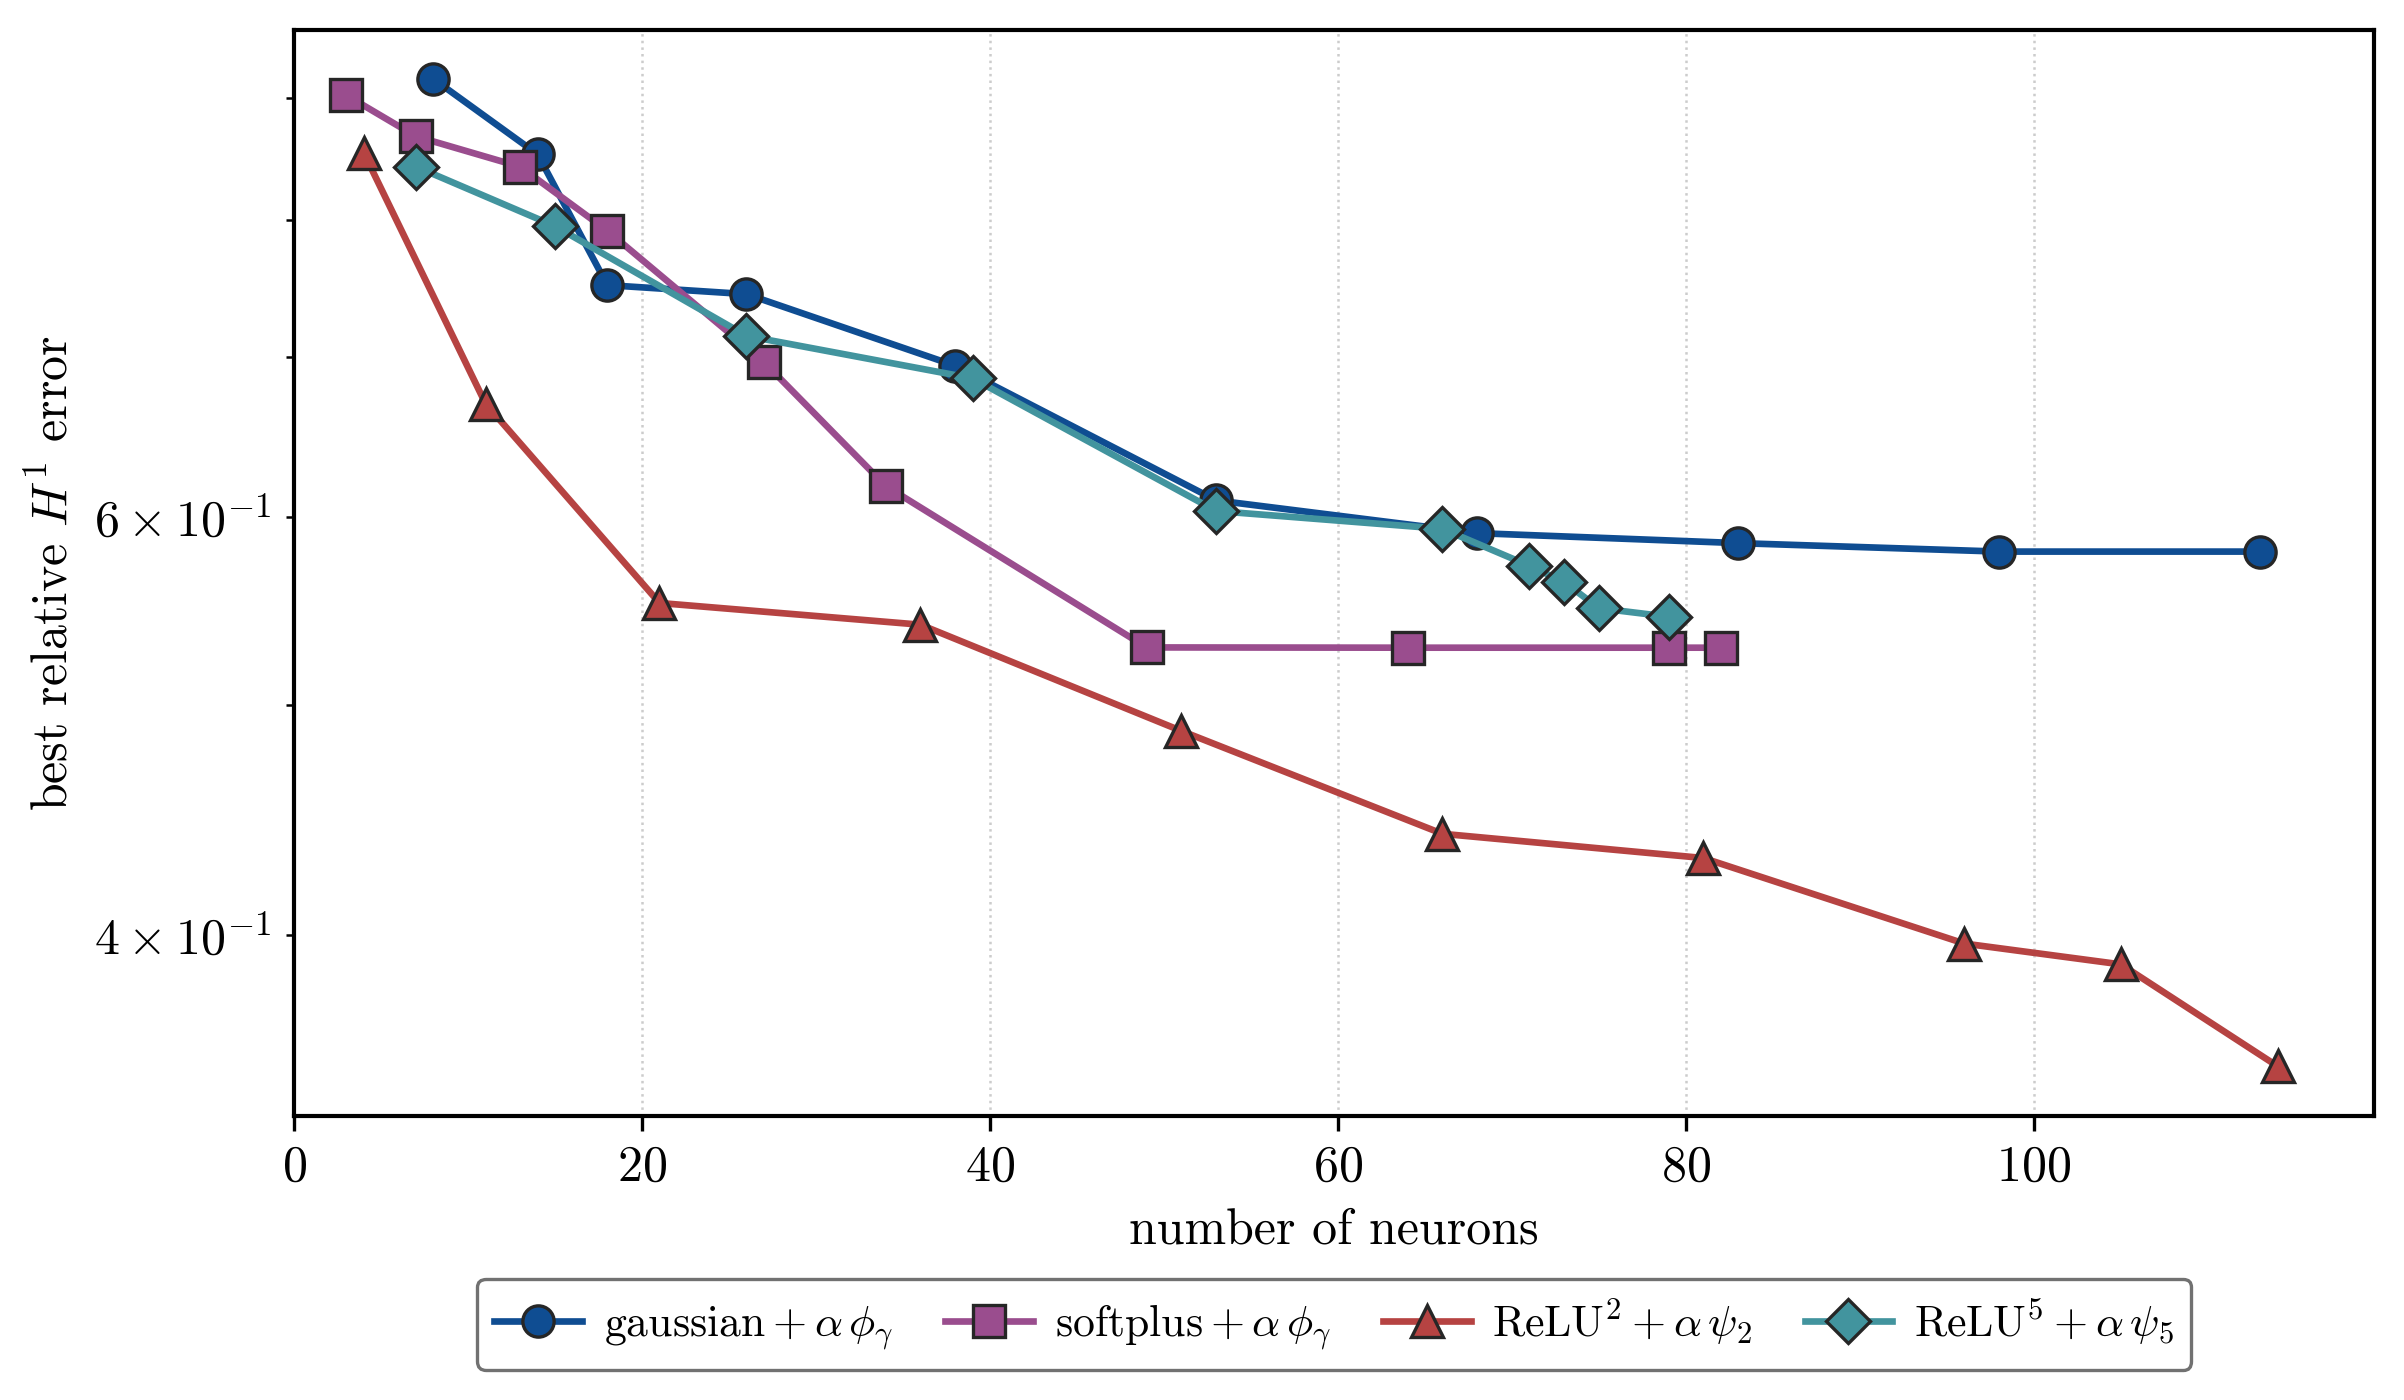
\includegraphics[width=0.7\textwidth]{plot/pendulum_insertion_frontier.png}
\caption{Best relative $H^{1}$ validation error against
neuron count, one curve per activation--penalty pair
($\phi_{\gamma}$ the log penalty, $\psi_{k}$ the fractional-exponent penalty),
on the two-sided switching-set data.
$\mathrm{ReLU}^{2}$ reaches the lowest error overall by a wide margin;
softplus, the Gaussian, and $\mathrm{ReLU}^{5}$ plateau at $1.5$--$1.6\times$
its error.}
\label{fig:rs_frontier}
\end{figure}

Figure~\ref{fig:rs_atoms} draws each atom's active line $\{a\cdot x + b = 0\}$
in the physical $(\theta,\dot\theta)$ plane, with line strength proportional to
the outer weight $|c_{n}|$, for $\mathrm{ReLU}^{2}$ (left) and Gaussian (right);
the switching curve is shown in black. $\mathrm{ReLU}^{2}$ concentrates its
strongest ridges parallel to the diagonal switching arms --- piecewise
low-degree ridges whose derivative breaks exactly where the target's does ---
whereas the Gaussian spends its capacity on near-isotropic bumps that can tile
the wells but cannot seat a gradient break. This alignment is the mechanism
behind the frontier advantage above and behind the transect kink of
Figure~\ref{fig:rs_transect}.

\begin{figure}[H]
\centering

\includegraphics[width=0.85\textwidth]{plot/atom_portrait.png}
\caption{Active atom lines $\{a\cdot x + b = 0\}$ in the $(\theta,\dot\theta)$
plane (strength $\propto |c_{n}|$) for $\mathrm{ReLU}^{2}$ (left) and Gaussian
(right); the switching curve is black. $\mathrm{ReLU}^{2}$'s strongest ridges
run parallel to the switching arms; the Gaussian atoms tile the wells
isotropically.}
\label{fig:rs_atoms}
\end{figure}


In summary, $\mathrm{ReLU}^{2}$ with the fractional-exponent penalty is the
best atom class for this nonsmooth target. With the two-sided band the
switching set is an \emph{interior} kink of the training data, and the
experiment measures representation rather than extrapolation: every atom class
pays a several-fold accuracy penalty in the band around the curve, and only
$\mathrm{ReLU}^{2}$ --- whose derivative can break across a hyperplane ---
partially seats the jump (Figure~\ref{fig:rs_transect}). The two-sided
coverage also has a price: the band carries most of the squared mass of the
unweighted $H^{1}$ objective, so interior accuracy degrades relative to
training on the basin alone --- least for $\mathrm{ReLU}^{2}$, most for the
stiff high-power atoms. In closed loop the branch decision at the curve
becomes learnable, and $\mathrm{ReLU}^{2}$ alone makes it correctly from both
sides of the switching set, matching the optimal cost from the braking side;
the smooth models fail from both starts. The bottleneck has moved from data
coverage across the curve to the atoms' ability to represent the kink ---
which is precisely the regime the sparse rectified atoms are built for.


\newpage
\bibliographystyle{plain}
\bibliography{ref.bib}
\end{document}
